\documentclass[12pt, oneside, onecolumn]{book}
\newcommand\hmmax{0}
\newcommand\bmmax{0}
\usepackage[a4paper, top=2.5cm, bottom=1.8cm, left=2.5cm, right=2.5cm]{geometry}

\usepackage{fancyhdr} %Fancy Header
\renewcommand{\baselinestretch}{1.3}
\usepackage{titlesec} %Select alternative section titles - change font of headers with one command

\fancypagestyle{plain}{% <==============================================
	\fancyhf{}
	\fancyfoot[R]{\thepage}
	\renewcommand{\headrulewidth}{0pt}
	\renewcommand{\footrulewidth}{0pt}%
}
\usepackage{emptypage} %True empty page


\usepackage{latexsym} %Standard
\usepackage{amssymb} %Standard
\usepackage{amsbsy} %Standard
\usepackage[fleqn]{amsmath} %Standard
\setlength\mathindent{\parindent}
\usepackage{makeidx} %Standarad package for making indexes
\usepackage{subfigure} %sideByside figures, inedependet labelin
%\usepackage{ifthen} %Control flow
%\usepackage{algorithmic} %Control flow
%\usepackage{algorithm} %Control flow
\usepackage{enumerate} %Bulleting
\usepackage{txfonts} %More fonts
\usepackage{multirow} %Create tabular cells spanning multiple rows
\usepackage{setspace} %Set space between lines
\usepackage{tabularx} %Tabulars with adjustable-width columns
\usepackage{colortbl} %Add colour to LaTeX tables
\usepackage{hhline} %Better horizontal lines in tabulars and arrays
\usepackage{float} %Improved interface for floating objects e.g. figures - using h, H...
%\usepackage{tikz} %Powerful package for creating graphic elements
\usepackage{pgfplots} %Create normal/logarithmic plots in two and three dimensions
\usepackage{paralist} %Enumerate and itemize within paragraphs
\usepackage{rotating} %Rotation tools, including rotated full-page floats - landscape figure, why not?
\usepackage[utf8]{inputenc} %Accept different input encodings
\usepackage[croatian]{babel} %Multilingual support
\usepackage[croatian]{babelbib} %Multilingual bibliographies
\usepackage[T1]{fontenc} %Standard package for selecting font encodings
%\usepackage{pslatex} %Use PostScript fonts by default
%\usepackage{url} %Verbatim with URL-sensitive line breaks
\usepackage{pdfpages} %Include PDF documents in LaTeX
\usepackage{siunitx} %A comprehensive (SI) units package
%\usepackage[absolute]{textpos} %Place boxes at arbitrary positions on the LaTeX page
\usepackage{upgreek} %Upright Greek letters.... yeah more fonts
\usepackage{chemformula} %Command for typesetting chemical formulas and reactions
\usepackage{bm} %Package for making arguments bold
\usepackage{mathalfa} %Package for additional mathfonts - new name of package mathalpha - but this should work
\usepackage{graphicx} %Enhanced support for graphics - \includegraphics{}
\usepackage[math]{cellspace} %Ensure minimal spacing of table cells
\cellspacetoplimit 1.pt
\cellspacebottomlimit 1pt
\setlength{\arraycolsep}{2pt}


\usepackage{mathtools} %Mathematical tools to use with amsmath - prettier math docs
\usepackage{courier} %More fonts just in case
\usepackage{enumitem} %Control layout of itemize, enumerate, description
\usepackage{array} %Extending the array and tabular environments
\usepackage{listings} %Typeset source code listings using LaTeX - see prilog for matlab.... use google for other languages, or set it up to your prefernce
\usepackage{color} %Colour control for LaTeX documents
\definecolor{mygreen}{RGB}{0,128,0} % Red, Green, Blue
\definecolor{mylilas}{RGB}{128,0,128} 
\usepackage{lipsum} %Example Text
\usepackage{longtable} %Breakable table
%\lstset{basicstyle=\footnotesize\ttfamily,breaklines=true}
%\lstset{framextopmargin=50pt,frame=bottomline}
%
%\newcolumntype{L}{>{\raggedright\arraybackslash}p{12cm}<{}}



%% Reynolds number and stuff
\newcommand{\Arch}{\operatorname{\mathit{A\kern-.06em r}}} % http://de.wikipedia.org/wiki/Archimedes-Zahl
\newcommand{\Biot}{\operatorname{\mathit{B\kern-.06em i}}} % http://de.wikipedia.org/wiki/Biot-Zahl
\newcommand{\Cauc}{\operatorname{\mathit{C\kern-.07em a}}} % http://de.wikipedia.org/wiki/Cauchy-Zahl
\newcommand{\Damk}{\operatorname{\mathit{D\kern-.06em a}}} % http://de.wikipedia.org/wiki/Damk%C3%B6hler-Zahl
\newcommand{\Eule}{\operatorname{\mathit{E\kern-.03em u}}} % http://de.wikipedia.org/wiki/Euler-Zahl
\newcommand{\Four}{\operatorname{\mathit{F\kern-.10em o}}} % http://de.wikipedia.org/wiki/Fourier-Zahl
\newcommand{\Frou}{\operatorname{\mathit{F\kern-.07em r}}} % http://de.wikipedia.org/wiki/Froude-Zahl
\newcommand{\Gras}{\operatorname{\mathit{G\kern-.05em r}}} % http://de.wikipedia.org/wiki/Grashof-Zahl
\newcommand{\Karl}{\operatorname{\mathit{K\kern-.11em a}}} % http://de.wikipedia.org/wiki/Karlovitz-Zahl
\newcommand{\Knud}{\operatorname{\mathit{K\kern-.11em n}}} % http://de.wikipedia.org/wiki/Knudsen-Zahl
\newcommand{\Lewi}{\operatorname{\mathit{L\kern-.05em e}}} % http://de.wikipedia.org/wiki/Lewis-Zahl
\newcommand{\Mach}{\operatorname{\mathit{M\kern-.10em a}}} % http://de.wikipedia.org/wiki/Mach-Zahl
\newcommand{\Nuss}{\operatorname{\mathit{N\kern-.09em u}}} % http://de.wikipedia.org/wiki/Nusselt-Zahl
\newcommand{\Pecl}{\operatorname{\mathit{P\kern-.08em e}}} % http://de.wikipedia.org/wiki/P%C3%A9clet-Zahl
\newcommand{\Pran}{\operatorname{\mathit{P\kern-.03em r}}} % http://de.wikipedia.org/wiki/Prandtl-Zahl
\newcommand{\Rayl}{\operatorname{\mathit{R\kern-.04em a}}} % http://de.wikipedia.org/wiki/Rayleigh-Zahl
\newcommand{\Reyn}{\operatorname{\mathit{R\kern-.04em e}}} % http://de.wikipedia.org/wiki/Reynolds-Zahl
\newcommand{\Schm}{\operatorname{\mathit{S\kern-.07em c}}} % http://de.wikipedia.org/wiki/Schmidt-Zahl
\newcommand{\Sher}{\operatorname{\mathit{S\kern-.07em h}}} % http://de.wikipedia.org/wiki/Sherwood-Zahl
\newcommand{\Stro}{\operatorname{\mathit{S\kern-.07em r}}} % http://de.wikipedia.org/wiki/Strouhal-Zahl
\newcommand{\Webe}{\operatorname{\mathit{W\kern-.14em e}}} % http://de.wikipedia.org/wiki/Weber-Zahl



%Za srediti naslove, podnaslove....
\titleformat{\chapter}{\normalfont\Large\bfseries\raggedright}{\thechapter.}{1em}{} 
\titleformat{\section}{\normalfont\large\bfseries\raggedright}{\thesection.}{2em}{} 
\titleformat{\subsection}{\normalfont\large\mdseries\raggedright}{\thesubsection.}{3em}{}  
\titleformat{\subsubsection}{\normalfont\normalsize\bfseries\raggedright}{\thesubsubsection.}{1em}{}
%Definiranje prostora oko naslova, podnaslova...
\titlespacing*{\chapter}{0pt}{-20pt}{30pt}
\titlespacing*{\section}{\parindent}{3ex}{1.5em}
\titlespacing*{\subsection}{\parindent}{2ex}{1em}




\usepackage{tocloft} %Prettier Table of Content
\renewcommand\cftloftitlefont{\LARGE\bfseries}  


%External links
\definecolor{cite}{rgb}{0, 0, 139}% dark blue
\definecolor{link}{rgb}{0,0,255}% blue
\usepackage[linktocpage=true]{hyperref}
\hypersetup{
	colorlinks=true,
  linkcolor  = link,
  citecolor  = cite,
  urlcolor   = link,
  colorlinks = true,
}
\usepackage{bookmark} %A new bookmark (outline) organization for hyperref
\usepackage{hypdestopt} %Hyperref destination optimizer
\usepackage[labelfont=bf, format=hang, singlelinecheck=false, labelsep=period, justification=raggedright]{caption} %Nice caption
\usepackage{placeins} %Control float placement --> using \FloatBarrier floats won't go e.g. into a another section

%Counter
\usepackage{etoolbox} %e-TeX tools for LaTeX
\newcounter{citenum}
\def\oldcite{}
\let\oldcite=\bibcite
\def\bibcite{\stepcounter{citenum}\oldcite}
\newcounter{totfigures}
\newcounter{tottables}
\newcounter{totequations}
\makeatletter
\AtEndDocument{%
  \addtocounter{totfigures}{\value{figure}}%
  \addtocounter{tottables}{\value{table}}%
  \addtocounter{totequations}{\value{equation}}%
  \immediate\write\@mainaux{%
    \string\gdef\string\totfig{\number\value{totfigures}}%
    \string\gdef\string\tottab{\number\value{tottables}}%
    \string\gdef\string\toteq{\number\value{totequations}}%
    \string\gdef\string\totcite{\number\value{citenum}}%
  }%
}
\makeatother

\pretocmd{\chapter}{\addtocounter{totfigures}{\value{figure}}\setcounter{figure}{0}}{}{}
\pretocmd{\chapter}{\addtocounter{tottables}{\value{table}}\setcounter{table}{0}}{}{}
\pretocmd{\chapter}{\addtocounter{totequations}{\value{equation}}\setcounter{equation}{0}}{}{}







%%%%%%%%%%%%%%%%%%%%%%%%%% DOKUMENT %%%%%%%%%%%%%%%%%%%%%%%%%%%%%%%%%%%%%%%%%%%%%%%%%
\begin{document}
	%\pagenumbering{roman}
	\pagestyle{fancy}
	\fancyhead{}
%	\fancyhead[C]{\leftmark}
	\fancyfoot{}
	\fancyhead[C]{Sveučilište u Splitu}
	\fancyhead[R]{FESB}
	\fancyhead[L]{Ante Svalina}
	\fancyfoot[R]{\thepage}
	
	\setstretch{1.0}
	\linespread{1.6}
	\setlength{\parindent}{0em}
	\setlength{\parskip}{0.8em}
	
	%Prostor oko jednadžbi slika, tablica
	\addtolength{\abovedisplayskip}{-2mm}
	\addtolength{\abovedisplayshortskip}{-2mm}
	\addtolength{\belowdisplayskip}{-2mm}
	\addtolength{\belowdisplayshortskip}{-2mm}
	\setlength{\abovecaptionskip}{1mm}
%%%%%%%%%%%%%%%%%%%% NASLOVNICA / FRONT COVER PAGE %%%%%%%%%%%%%%%%%%%%%%%%

\begin{titlepage}
	\begin{center}	
		{\fontsize{18}{20}\textbf{S V E U Č I L I Š T E \ \  U \ \  S P L I T U}}
		\par
		\vspace{1cm}
		{\fontsize{18}{20}\textbf{FAKULTET ELEKTROTEHNIKE, STROJARSTVA I BRODOGRADNJE}}
		\vspace{6cm}
		\par
		{\fontsize{18}{20}\bfseries{DIPLOMSKI RAD}}
		\par
		\vspace{3cm}
		{\fontsize{22}{26}\bfseries{PIV sustav mjerenja brzine strujanja}}
		\vspace{1cm}
		\par
		{\fontsize{18}{20}\textbf{Ante Svalina}}
		\vspace{8cm}
		\par
		{\Large Split, rujan 2021.}
	\end{center}
\end{titlepage}


\includepdf[pages={1}]{Zadatak_Ante_Svalina.pdf}
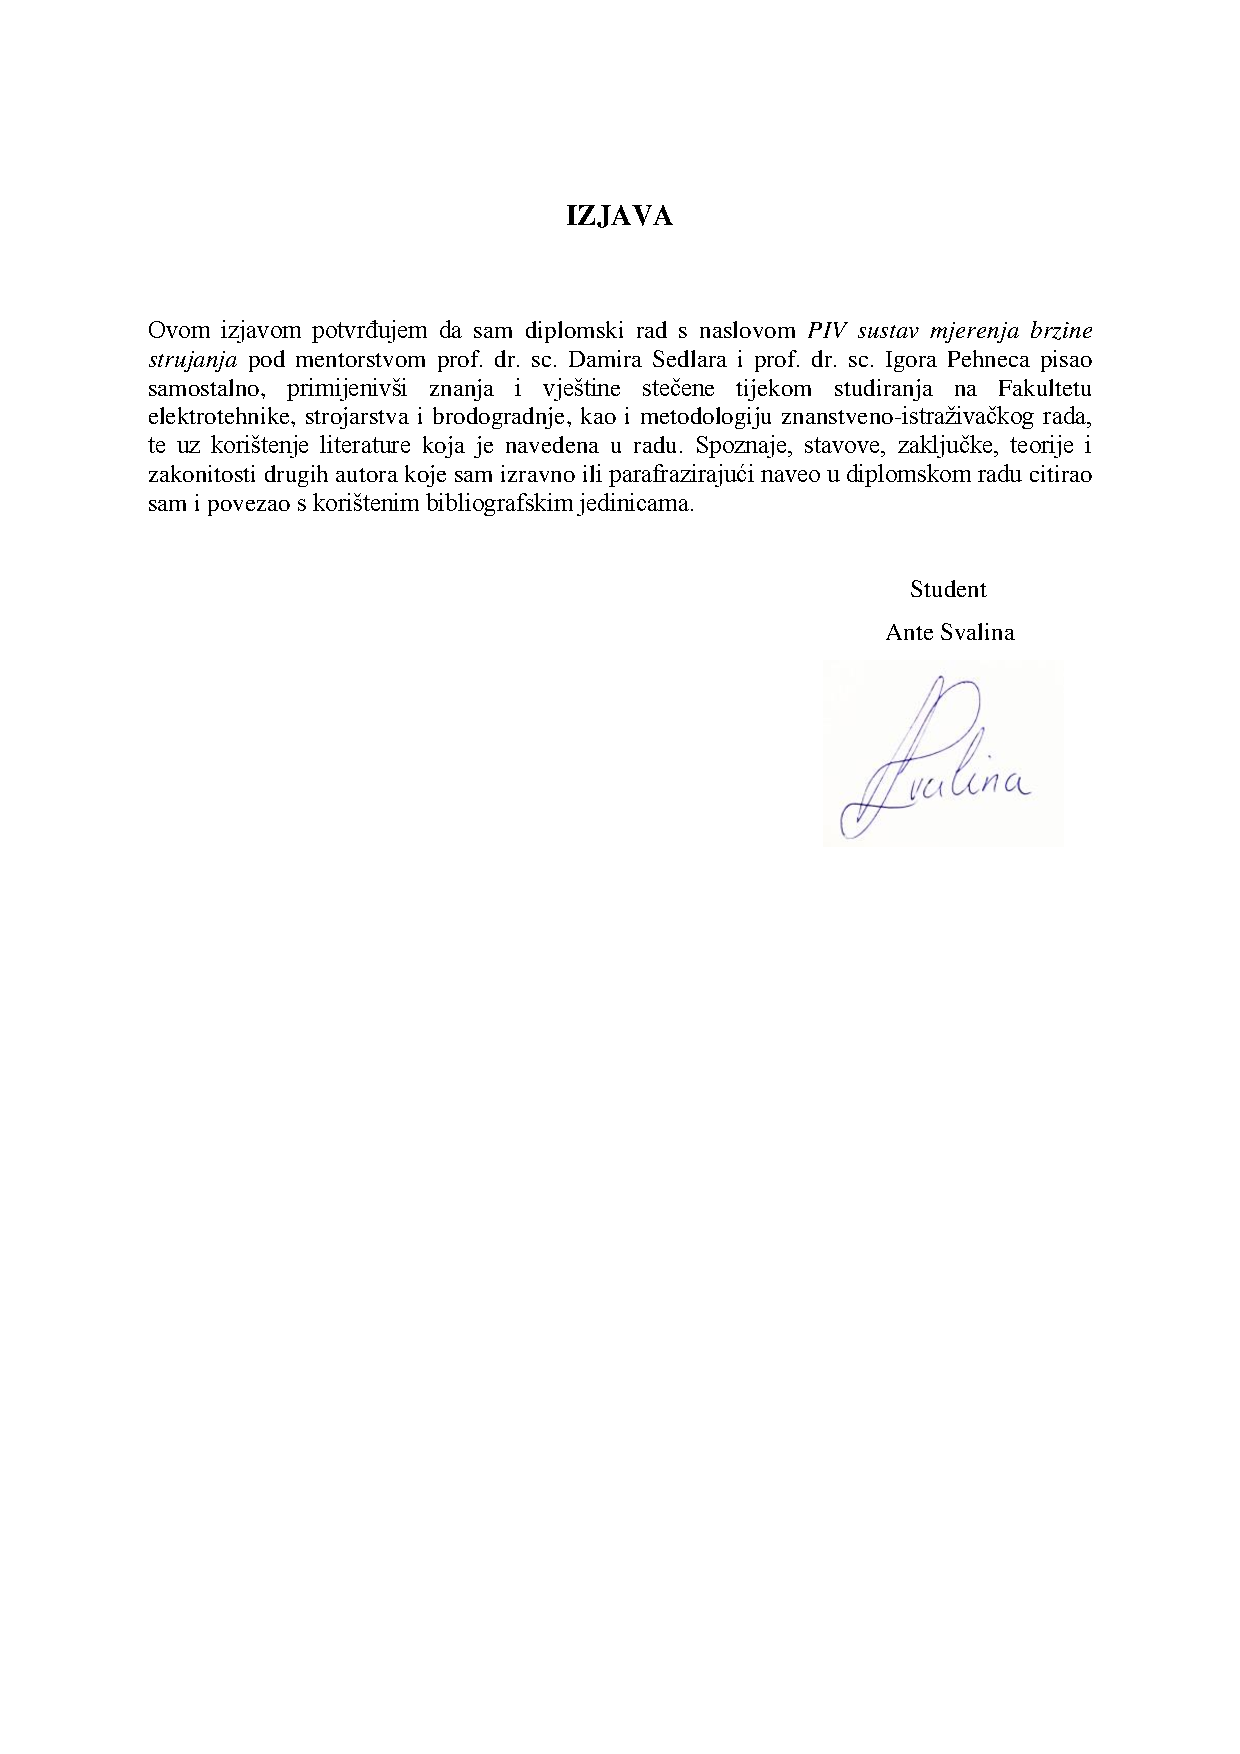
\includepdf[pages={1}]{izjavaDipl.pdf}
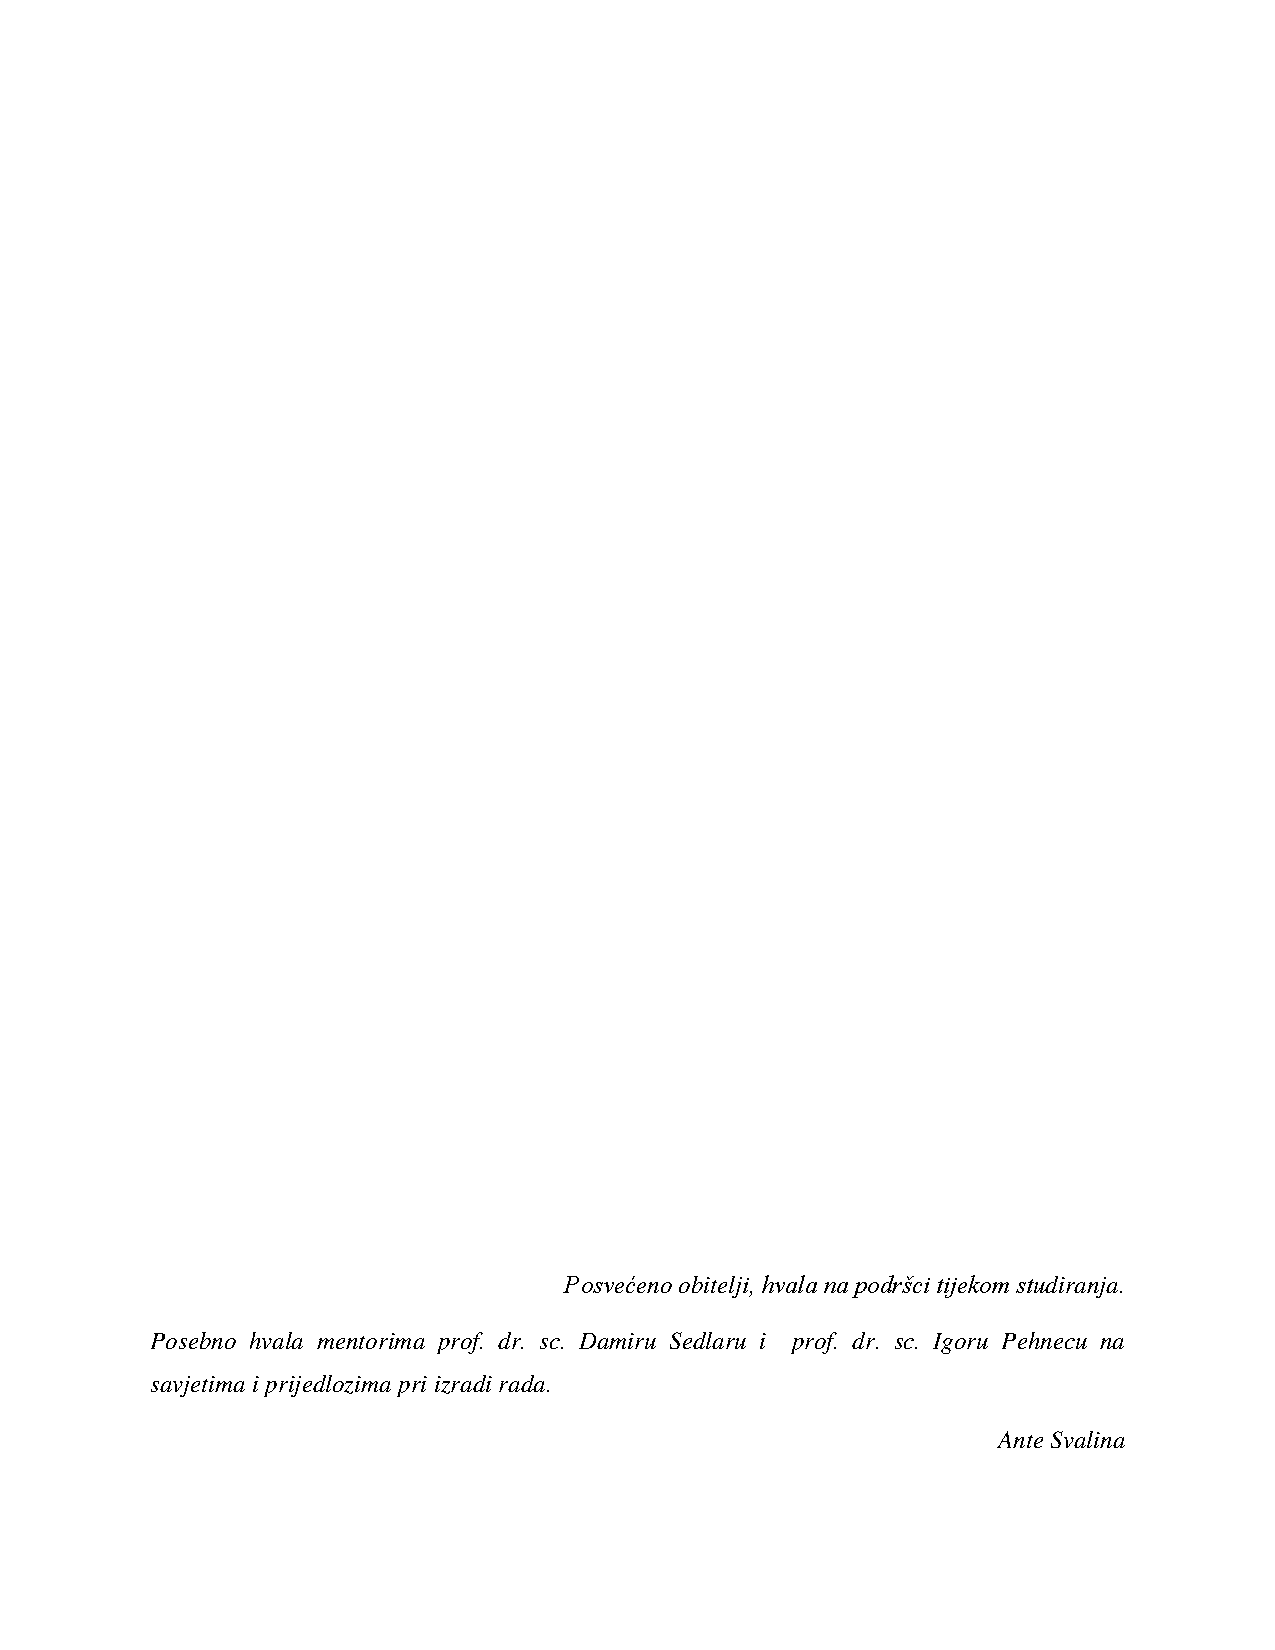
\includepdf[pages={1}]{zahvala.pdf}



\frontmatter
%%%%%%%%%%%%%%%%%%%%%%%%%%%%%%%%% TOC %%%%%%%%%%%%%%%%%%%%%%%%%%%%%%%%%%%%%
\tableofcontents





\mainmatter
%%%%%%%%%%%%%%%%%%%%%%%% POGLAVLJA / CHAPTERS %%%%%%%%%%%%%%%%%%%%%%%%%%%%%

\chapter{UVOD}
\label{chap:Poglavlje_1}

Eksperimentalna mehanika fluida redovno zahtijeva kvantitativnu vizualizaciju, te sveukupno mjerenje svojstava fluidne domene. Metode mjerenja brzine strujanja poput, mjerenja žarnom niti i laserske Doppler anemometrije (LDA), imaju nepremostivo ograničenje u mjerenju brzine u samo jednoj točki domene istodobno. Zadnjih tridesetak godina u industriji i istraživačkom radu se zbog ubrzanog razvoja računalne i digitalne tehnike ubrzano razvija DPIV tehnika mjerenje koja ima mogućnost nerazarajućeg trenutnog mjerenja diskretnog polja brzine. U PIV mjerenjima posredno se prati brzina osvjetljenih čestica. DPIV tehnikom omogućeno je ravninsko (2D) mjerenje fluida, pri čemu su potrebne određene komponente uz pomoć kojih se ostvaruje mjerenje: kamera za snimanje, osvjetljenje, čestice markeri koji služe kao vizualni indikator, te softver za analizu i mjerenje dobivenih snimki. U novije doba moguće je 3D PIV mjerenje pri čemu je samo potrebna druga kamera koju je jednostavno dodatno implementirati u 2D sustav (stereo-PIV).
\par
Cilj je ovog rada pojašnjenje principa funkcioniranja DPIV analize, te prikaz procesa konstrukcije i korištenja jednostavnog PIV sustava. U radu su objašnjeni najnapredniji DPIV algoritmi, te je dan kratak opis mogućih problema prilikom PIV mjerenja. Matematički je opisana i pojašnjena kros-korelacija koja je "srce" DPIV analize, te je u MATLABU napravljen vlastiti program uz pomoć kojeg je jednostavno shvatiti poantu i prednosti statističke kros-korelacijske analize za razliku od drugih mogućih metoda praćenja kretanja čestica (PTV). Uz rizik pretjeranog pojednostavljenja, ideja kros-korelacije je mjerenje sličnosti između dva uzorka, gdje se korelacijom jednog s drugim dobivaju određene vrijednosti koje govore o intenzitetu poklapanja dva uzorka.
\par
Kako je glavni cilj svakog eksperimentalnog mjerenja minimizacija greški između stvarnih i mjerenih veličina, kvaliteta rada DPIV softvera najviše se odražava u točnosti njegove analize. Zbog toga su u radu generirane umjetne PIV snimke uz pomoć kojih je prikazana metodologija evaluacije PIV točnosti. Generirani parovi snimki analizirani su u vlastitom kros-korelacijskom programu, te uspoređeni s analizom u robusnom PIVlab softveru kako bi se kvalitativno i kvantitativno odredile značajke korelacijske analize.
\par
Rad je napravljen s namjerom razumijevanja svih DPIV tehnika. Većina današnjih DPIV alata, kako komercijalnih, tako i open-source, uglavnom su "crne-kutije" koje ulazne podatke često obrade bez da korisnik detaljno razumije moguće probleme analize što može dovesti do grešaka koje se ne smiju zanemariti. Također, razumijevanje funkcioniranja DPIV softvera omogućuje vlastito pojedinačno prilagođavanje i optimiranje postavki analize potrebama promatranog eksperimenta.






\chapter{TEORETSKA POZADINA DPIV ANALIZE}
\label{chap:Poglavlje_2}

Digitalno mjerenje brzine foto-gramom čestica (\textit{eng. DPIV - Digital Particle Image Velocimetry}) je tehnika neinvazivne kvalitativne i kvantitativne optičke vizualizacije strujanja fluida. Malene čestice markeri (\textit{eng. TP - Tracer Particles}) koje imaju neutralni uzgon ubace se u struju tekućine ili plina, te služe kao vizualni indikator gibanja fluida. Bolja vizualizacija se postiže osvjetljivanjem protoka uz pomoć tanke (uobičajeno zelene) laserske ravnine (2D PIV). Laserska svjetlost obasja čestice markere, te dolazi do raspršivanja svjetlosti, što omogućuje bolju vizualizaciju protoka. Digitalni fotografski senzor pozicioniran je paralelno sa osvijetljenom plohom, te je na taj način moguće fotografiranje i smrzavanje protoka čestica (\textit{Slika \ref{sl:2.1}}).
\begin{figure}[h]
	\centering
	%\usepackage{graphicx}
	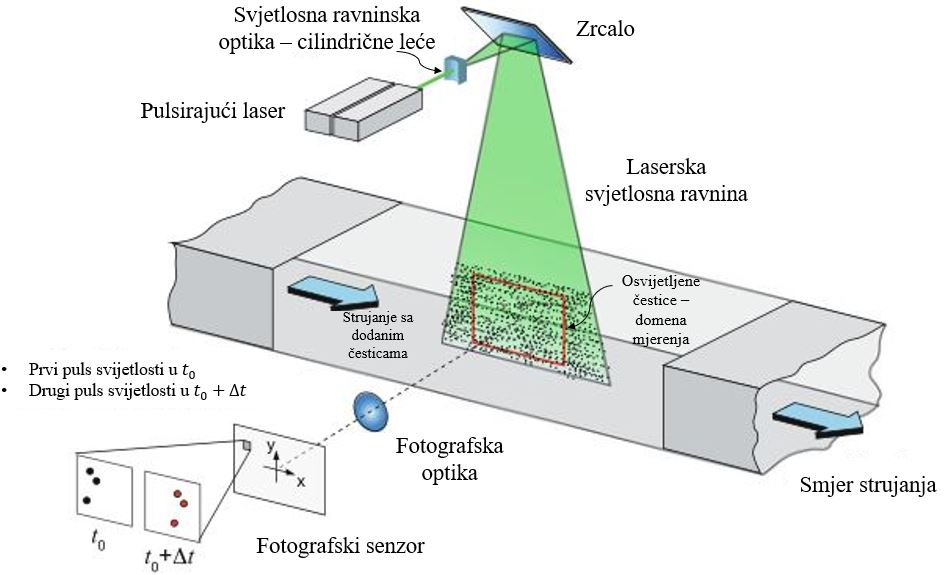
\includegraphics[width=14cm]{./2_DPIV/2_1PivSetup.jpg} 
	\caption{Eksperimentalni 2D PIV sustav \cite{raffel2018_book}}
	\label{sl:2.1}
\end{figure}
\par
U većini DPIV analiza snime se dvije fotografije (1 i 2) osvijetljene domene mjerenja u trenutcima $t_0$ i $t_0+\Delta t$. Brzine se stoga mogu dobiti uz pomoć parametara $\Delta t$ i udaljenosti koje su čestice prošle između dvije snimke 1 i 2 (pomak čestica). U DPIV pomak čestica proračunava se tako da se domena mjerenja podijeli u manja "prozore" mjerenja tzv. područja ispitivanja (\textit{eng. interrogation areas}). Svako područje ispitivanja sadrži svoju grupu čestica. Nakon podijele domene provodi se statistička analiza uz pomoć kros-korelacije (\textit{eng. cross-correlation}) svih podijeljenih prozora ispitivanja. Korelacija daje najvjerojatniji pomak grupe čestica koje se gibaju u ravnoj liniji između slika 1 i 2.
DPIV analiza ukratko se može podijeliti na 4 glavna koraka \cite{thielicke2014_article}: 
\begin{enumerate}[topsep=0pt, itemsep=0em]
	\item Akvizicija slika
	\item Pretprocesiranje slika (Softversko poboljšanje slika)
	\item Evaluacija slika
	\item Postprocesiranje PIV podataka
\end{enumerate}
\FloatBarrier
\section{Akvizicija slike}
Kako je PIV vizualna tehnika za analizu čestica, što znači da se PIV tehnikom brzina strujanja mjeri indirektno, prvi korak PIV procesa počinje fotografiranjem osvijetljene domene u koju su dodane čestice markeri. Da bi se omogućila što veća točnost PIV analize trebalo bi osigurati da dobivene slike budu što bolje kvalitete i da sadrže što manje šuma. U ovom radu prikazani su neki od najbitnijih parametara koji bi se trebali uzeti u obzir kod akvizicije slike. 
\subsection{Odabir čestica markera}
Fluidi su u većini slučajeva homogeni, pa je stoga brzine teško izmjeriti optičkim sredstvima. Zbog toga se uobičajeno u fluid dodaju razne reflektirajuće čestice. Obično odabir čestica kod tekućina ne predstavlja preveliki problem, međutim kod vizualizacije strujanja zraka, teško je pronaći čestice koje imaju sličnu gustoću kao i zrak. Prilikom odabira čestica treba uzeti u obzir sljedeće čimbenike i pretpostavke  \cite{raffel2018_book}:
\begin{description}[style=unboxed,leftmargin=0cm]
	\item[Distribucija čestica markera u struji fluida.] Poželjno je da distribucija čestica bude što homogenija.
	\item[Gustoća distribucije čestica markera unutar domene]. Na \textit{Slici \ref{sl:2.2}} mogu se primijetiti 3 različita tipa gustoće čestica, za koji bi se trebali primijeniti različite tehnike obrade.
	\begin{figure}[h]  
		\centering
		%\usepackage{graphicx}
		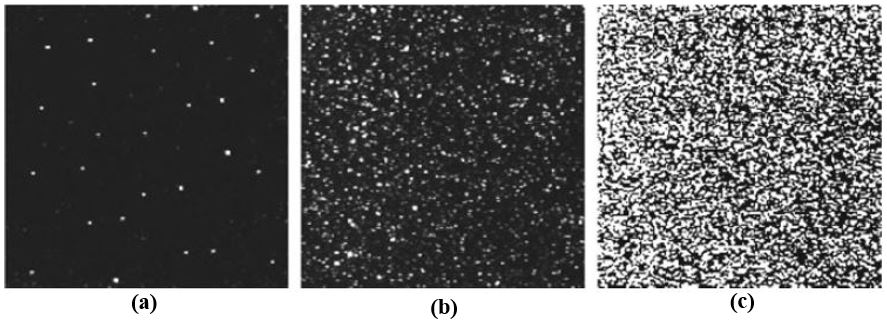
\includegraphics[width=14cm]{./2_DPIV/2_2GustocaDistribucijeCestica.jpg} 
		\caption{Tri moguća načina gustoće distribucije čestica \cite{raffel2018_book}:\\ \textbf{(a)} Niska gustoća (PTV)\\ \textbf{(b)} Srednja gustoća (PIV)\\ \textbf{(c)} Visoka gustoća čestica (LSV)}
		\label{sl:2.2}
	\end{figure}
	U slučaju niske gustoće (\textit{Slika \ref{sl:2.2}a}), moguća je detekcija i praćenje svake čestice zasebno. Radi toga niska gustoća distribucije za analizu zahtjeva neke od metoda praćenja objekata (markera). Stoga se ovaj način mjerenja naziva "\textit{mjerenje brzine praćenjem čestica}" (\textit{eng. PTV - Particle Tracking Velocimetry}). Za slučaj srednje gustoće distribucije čestica (\textit{Slika \ref{sl:2.2}b}) i dalje se može primijetiti svaka individualna čestica, međutim više nije moguće njihove praćenja zbog nesigurnosti da li je uistinu praćena čestica na sljedećoj slici ispravno i nedvosmisleno uočena. Ovakve fotografije analiziraju se uz pomoć statističkih PIV metoda (kros-korelacija). Kod slika sa visokom gustoćom distribucije čestica (\textit{Slika \ref{sl:2.2}c}) više nije moguće primijetiti svaku česticu posebno pošto dolazi do preklapanja i formiranja "mrlja" (\textit{eng. speckles}). U ovom slučaju mjerenje i analiza ovakvih fotografija naziva se "\textit{Laser Speckle Velocimetry}" (LSV).
	\item[Zaostajanje brzine (\textit{eng. velocity lag}).] Prilikom odabira čestica treba obratiti pažnju da li čestice vjerno prate gibanje svakog fluidnog elementa, barem do razine gdje se može zaključiti kako će rezultati mjerenja biti zadovoljavajući. Kod promatranja velikih domena strujanja, gdje se pojavljuju i veliki i mali gradijenti brzina, treba se pronaći kompromis između biranja većih i manjih čestica. Veće čestice će bolje raspršiti svjetlost, te će se vidjeti cijelo promatrano polje strujanja, ali ipak lokalno, mjesta gdje ima velikih promjena brzine će ostati neriješena. Glavni i najvažniji izvor grešaka kod korištenja čestica markera javlja se zbog djelovanja akceleracijskih sila (npr. gravitacija, centrifugalne sile) na česticu koja ima različitu gustoću od fluida, te će zbog toga ukratko biti objašnjen utjecaj ubrzanja \cite{raffel2018_book}. Kako postoji razlika u gustoćama između fluida $\rho$ i čestica tragača $\rho_\textup{č}$ prikazan je izraz za Stokes-ov zakon otpora \cite{Pehnec2020Predavanja} koji prikazuje zaostajanje brzine $\boldsymbol{U}_s$ između brzine čestice $\boldsymbol{U}_\textup{č}$ i brzine fluida $\boldsymbol{U}$. U izrazu se pretpostavlja da je čestica sfernog oblika, te struji u viskoznom fluidu pri jako malom Reynolds-ovom broju:
	\begin{equation}
		\boldsymbol{U}_{s}=\boldsymbol{U}_\textup{č}-\boldsymbol{U}=d_\textup{č}^2\dfrac{\rho_\textup{č}-\rho}{18\mu}\boldsymbol{a}
		\label{eqn:2.1}	
	\end{equation}
	gdje je $d_\textup{č}$ - promjer čestice, $\rho_\textup{č}$ - gustoća čestice, $\rho$ - gustoća fluida, $\mu$ - dinamička viskoznost fluida, $\boldsymbol{a}$ - ubrzanje.
	\par
	U slučaju naglog usporenja i velike razlike između gustoća fluida i čestica vremenski odziv $t$ brzine čestice $\boldsymbol{U}_\textup{č}$ ima trend eksponencijalnog raspada:
	\begin{equation}
		\boldsymbol{U}_\textup{č}(t)=\boldsymbol{U}\left[1-\exp\left(-\dfrac{t}{\tau_\textup{č}}\right)\right]
		\label{eqn:2.2}	
	\end{equation}
	gdje vrijeme odziva $\tau_\textup{č}$ glasi:
	\begin{equation}
		\tau_\textup{č}=d_\textup{č}^2\dfrac{\rho_\textup{č}}{12\mu}
		\label{eqn:2.3}
	\end{equation}
	Ako ubrzanje fluida nije konstantno ili Stokes-ov zakon otpora ne vrijedi (npr. za velike čestice ili veće brzine strujanja), rješenje jednadžbe \ref{eqn:2.3} više nije jednostavni eksponencijalni raspad. Razlog je u tome što jednadžbe strujanja (Navier-Stokes-ove jednadžbe) postaju nelinearne i sve su teže rješive. No unatoč tome $\tau_\textup{č}$ se i dalje može smatrati prikladnom mjerom za težnju čestice da uspostavi brzinsku ravnotežu sa fluidom. Na slici \ref{sl:2.3} prikazano je teoretsko vrijeme odziva (jednadžba \ref{eqn:2.2}) čestica različitih promjera kod "kvazi-trenutačnog" usporenja prilikom strujanja u zraku \cite{raffel2018_book}.
	\begin{figure}[h]  
		\centering
		%\usepackage{graphicx}
		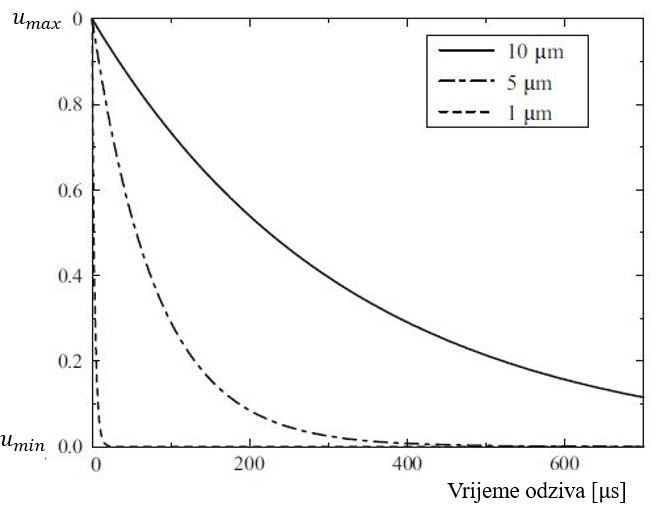
\includegraphics[width=9cm]{./2_DPIV/2_3VrijemeOdzivaCestica.jpg} 
		\caption{Teoretsko vrijeme odziva raspršenih uljnih čestica različitog promjera u zraku \cite{raffel2018_book}}
		\label{sl:2.3}
	\end{figure}
	\item[Utjecaj Brown-ovog gibanja.] U slučaju da su čestice markeri iznimno malog promjera (manje od 1 $\mu$m) može doći do tzv. Brown-ovog gibanja, gdje dolazi do efekta sudaranja, te miješanja čestica i fluida na mikro razinama (npr. gibanje čestica dima u zraku). Ovaj fenomen obično se pojavljuje pri $\mu$PIV mjerenjima, te dovodi do greški u kros-korelacijskoj analizi, zbog nesigurnosti u položaj čestica.
\end{description}
\FloatBarrier
\subsection{Osvjetljenje}
Kao osvjetljenje u PIV eksperimentima uobičajeno se primjenjuju pulsirajući laseri, zbog svoje sposobnosti da emitiraju monokromatsko svijetlo visokog energetskog intenziteta. Točkasti snop laserske svjetlosti jednostavno je transformirati u tanku ravninu (plahtu) koristeći jednu ili više cilindričnih leća \cite{raffel2018_book}, a osvjetljenje i snimanje korištenjem laserske ravnine onemogućuje kromatske aberacije. Danas je dostupno mnogo različitih lasera koji koriste razne tipove laserskih materijala, te različite načine energetskog upumpavanja. U PIV svrhe zbog svoje kompaktnosti i visoke efikasnosti najčešće se koriste "\textit{diodno upumpavani laseri čvrstom jezgrom}" (\textit{eng. DPSSL - diode pumped solid state lasers}).
\par
Najkorišteniji tip DPSSL lasera u PIV mjerenjima je Neodym-Yttrium-Aluminium-Garnet laser (Nd:YAG). Nd:YAG je laser s krutom jezgrom \cite{wiki:Nd:YAG} koji se sastoji od štapića itrij-aluminijevog granata (YAG), dopiranog atomima neodimija (Nd:\ch{Y3Al5O12)}. Radna valna duljina ovog lasera je 1064 nm (infracrveno zračenje), ali frekvencijskim dupliranjem, zraka koja napušta laser može se podesiti na valnu duljinu od 532 nm što odgovara zelenom spektru zračenja. Nd:YAG laseri mogu biti korišteni u pulsirajućem i kontinuiranom modu. Pulsirajući laseri ostvaraju veoma visoke snagu tijekom vrlo kratkih impulsa, što omogućuje smanjivanje efektivnog vremena ekspozicije kamere. Dok kontinuirani laseri zahtijevaju dulja vremena ekspozicije kako bi ostvarili zadovoljavajuću količinu svjetla, a dulja ekspozicija dovodi do pretjeranog zamućenja gibanja čestice. Zamućene čestice nisu poželjne zbog kvalitete kros-korelacijske obrade (poželjno je da svaka slika doslovno zamrzne gibanje čestica). Ipak prednost kontinuiranih lasera je u tome da ne zahtijevaju dodatni hardware za sinkronizaciju sa brzim kamerama, za razliku od pulsirajućih lasera, gdje je sinkronizacija kamere i lasera neizbježna.
\subsection{Snimanje}
Osvijetljena ravnina u PIV analizi snimana je kamerom kojoj optička os "udara" okomito na osvijetljenu ravninu. Za PIV snimke generalno su potrebne jako kvalitetne leće zbog toga što leveli svjetlosti znaju biti relativno niski, te su potrebni veliki otvori blende da uhvate što više svjetla. Znatan napredak PIV analize omogućen je pojavom digitalnih kamera sa CCD ili CMOS foto čipovima. Ove kamere omogućile su instant analizu strujanja i povratnu informaciju o kvaliteti slike. Elektronske kamere dostupne su cijelom području rezolucija, osjetljivosti, brzine zatvarača (\textit{eng. shutter speed}), brzine snimanja (\textit{eng. frame rate}), itd.. Prilikom odabira kamere za određena PIV mjerenja treba uzeti u obzir sljedeće eksperimentalne karakteristike: područje brzina strujanja koje se promatraju, ponovljivost eksperimenta, te intenzitet osvjetljenja. U \textit{Tablici \ref{tab:2.1}} prikazan je općeniti sažetak najčešćih eksperimentalnih situacija, te tipa kamere koji se preporučuje koristiti.
\begin{table}[h]
	\centering
	\caption{Preporuka pri odabiru kamere za PIV mjerenja ovisno o brzini strujanja, ponovljivosti eksperimenta i jačini osvjetljenja \cite{stamhuis2006basics}}
	\begin{tabular}{|c|c|c|c|}
		\hline
		\rowcolor[HTML]{9B9B9B} 
		\begin{tabular}[c]{@{}c@{}}\textbf{Brzina} \\ \textbf{strujanja}\end{tabular} & \begin{tabular}[c]{@{}c@{}}\textbf{Intenzitet} \\ \textbf{osvijetljenja}\end{tabular} & \textbf{Ponovljivost} & \textbf{Tip kamere}                                                                                                                  \\ \hline
		&                                                                     & Dobra        & \begin{tabular}[c]{@{}c@{}}Kamera sa dvostrukom \\ (višestrukom) ekspozicijom\end{tabular}                                  \\ \cline{3-4} 
		\multirow{-2}{*}{Brzo}                                      & \multirow{-2}{*}{Visok}                                             & Loša         & Brza kamera                                                                                                                 \\ \hline
		&                                                                     & Dobra        &                                                                                                                             \\ \cline{3-3}
		\multirow{-2}{*}{Sporo}                                     & \multirow{-2}{*}{Nizak}                                             & Loša         & \multirow{-2}{*}{\begin{tabular}[c]{@{}c@{}}Progressive scan kamera \\ (normalna ili srednja brzina snimanja)\end{tabular}} \\ \hline
	\end{tabular}
\label{tab:2.1}
\end{table}
\par
Progresivne scan kamera omogućuje snimanje slika brzinom od 25-30 fps pa sve do 100 fps (\textit{frames per second}). Ove vrste kamera se zbog dugačkog perioda između kadrova koriste pri niskim PIV brzinama. Brze kamere imaju mogućnost snimanja do 1000 fps, te su ove kamere izvrsne za brza strujanja gdje nema ponovljivosti (npr. snimanje strujanja oko ptica). Korištenje brze kamere u PIV analize (za neke slučajeve) je poznato i kao vremenski razriješeni PIV (\textit{eng. time-resolved PIV}). Kamera sa dvostrukom ekspozicijom ima mogućnost snimanja dvije ekspozicije (kadra) unutar iznimno kratkog perioda. Nakon snimanja obje ekspozicije se prebace na računalo, te je kamera spremna za snimanje novog para dvije ekspozicije. Period između para dvije ekspozicije može biti ispod 500 ns, no zato period između parova ekspozicija je dosta duži (0.1 do 0.5 s), ovisno o sustavu transfera slika na računalo (ili unutarnju memoriju). Zbog toga više-ekspozicionirane snimke su prikladne za PIV u kojem su brzine strujanja visoke ali i postoje ponovljivi uzorci strujanja.
\FloatBarrier
\section{Pretprocesiranje slike}
U DPIV analizi treba omogućiti što kvalitetniju procjenu brzine kako bi se osigurala najveća moguća kvaliteta mjerenja \cite{thielicke2014_article}. Jedan od uobičajenih pristupa je digitalno poboljšanje slike prije nego se dogodi sami postupak korelacije. Varijacije intenziteta slike snažno utječu na signal korelacije. Mjesta gdje su čestice bolje osvijetljene imaju puno veći utjecaj u korelaciji od mjesta gdje su čestice manje osvijetljene. Također nejednoliko osvijetljenje (zbog ne-uniformne distribucije laserske svjetlosti, varijacija između laserskih impulsa, nepravilno oblikovanih čestica, kretanja izvan ravnine,...) unose šum u korelacijsku ravninu. Iz tog razloga ulazne slike se gotovo uvijek poboljšavaju prije same evaluacije. Glavni cilj poboljšanja slike je primjena raznih tehnika kako bi se dovelo do većeg kontrasta u slici, te do toga da intenzitet čestica u slici dovede do slične razine signala tako da sve čestice imaju sličan doprinos u korelacijskoj funkciji. U idealnim uvjetima PIV slike bi se trebale sastojati od svijetlih čestica promjera 2-3 pixela koje se nalaze na crnoj površini. Na taj način korelacijska efikasnost bi se mogla dovesti na sub-pixelsku točnost \cite{mendez2017pod}. U ovom potpoglavlju biti će objašnjeni neke od pretprocesorskih tehnika koje se koriste u ovom radu i implementirane su u PIVlab softver.
\par
Jedan od načina postizanja bolje kvalitete slike je stacionarno "\textit{oduzimanje pozadine}" (\textit{eng. background subtraction}). Ova tehnika  smanjuje učinke laserskog odbljeska i ostalih stacionarnih značajki slike. Može se izvesti tako da se pozadinska slika snimi prije samog dodavanja čestica markera, ili ako to nije moguće, izračunavanjem slike prosječnog ili  minimalnog intenziteta iz dovoljno velik broja PIV snimki (najmanje 20-50). \cite{raffel2018_book}.
\par
Drugi način poboljšanja slike je zasnovan na "\textit{visoko-propusnom filtriranju}" (\textit{eng. high-pass filtering}) poznatom kao i izoštravanje fotografije. Ovom tehnikom pozadinske varijacije sa malom prostornom frekvencijom se uklanjaju ostavljajući tako slike čestica nepromijenjene. U praksi ovo se radi na način da se izračuna nisko-propusna verzija originalne slike i oduzme se od svoje originalne slike. Bitno je da širina primijenjenog filtra (\textit{eng. filter kernel}) bude veća od promjera čestica ($k_{\textup{filtra}}>d_\textup{č}$).
\par
Zajedno sa visoko-propusnim filtriranjem često se koristi i \textit{binarizacija slike} (\textit{eng. image binarization}) poznato kao i "\textit{thresholding}". Kao rezultat se dobije slika (obično crno-bijela) gdje sve čestice imaju jednak intenzitet i samim time jedak doprinos korelacijskoj funkciji. Međutim ova tehnika dovodi do povećavanja nesigurnosti u mjerenju, pa bi se trebala koristiti s oprezom.
\par
Korištenje filtra niske širine, "\textit{nisko-propusnog filtra}" (\textit{eng. low-pass filter}) može biti prikladno za uklanjanje visoko frekvencijskog šuma (npr. šum fotoaparata, pixel anomalije,...).
\subsection{Prilagodljivo rastezanje kontrasta}
\textit{Prilagodljivo rastezanje kontrasta} \cite{wiki:Adaptive_histogram_equalization} ili \textit{prilagodljivo izjednačavanje histograma} (\textit{eng. AHE - adaptive histogram equalization}) je tehnika obrade slike kojom se poveća kontrast slike. Razlikuje se od običnog rastezanja kontrasta (\textit{Slika \ref{sl:2.4}}) u kojem se globalno poveća kontrast, pa dolazi do toga da je u nekim područjima slike, kontrast optimalno definiran, a u drugim područjima nastaje mnogo šuma. AHE radi na način da se računa više histograma koji odgovaraju određenom lokalnom području slike. Na taj način kontrast slike optimalno se poboljša za svako područje slike, međutim i dalje može doći do pretjeranog pojačanja šuma u relativno homogenim područjima slike. Kako bi se to spriječilo u PIVlab softveru koristi se varijanta AHE-a koja se naziva \textit{kontrast ograničeno prilagodljivo izjednačavanje histograma} (\textit{eng. CLAHE - contrast limited adaptive histogram equalization}). CLAHE algoritam je predstavljen 1987 kao algoritam koji bi povećao "čitljivost" medicinskih fotografija.
\begin{figure}[h]  
	\centering
	%\usepackage{graphicx}
	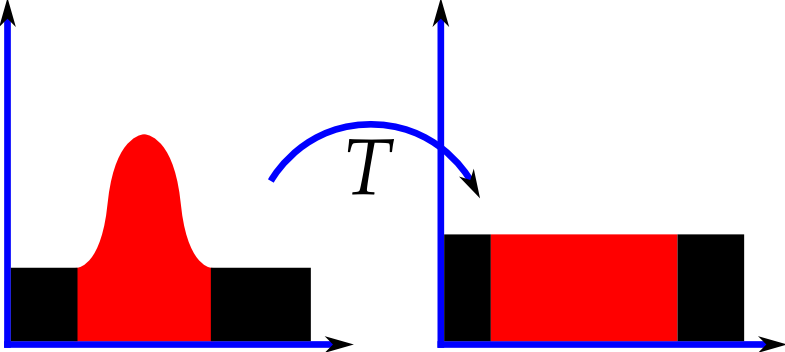
\includegraphics[width=8cm]{./2_DPIV/2_4Histogram.jpg} 
	\caption{Primjer histograma prije i nakon izjednačavanja \cite{wiki:Histogram_equalization}}
	\label{sl:2.4}
\end{figure}
\par
Prednost CLAHE algoritma u odnosu na AHE je da limitira pojačanje kontrasta u područjima koja nemaju nagle promjene. Ovo je jako bitno kod DPIV analize zbog toga što uniformna ekspozicija cijele slike često ne može biti osigurana \cite{adrian2011_book}, prvenstveno radi toga što laserska ravninska zraka ima normalnu (Gauss-ovu) distribuciju. U CLAHE-e algoritmu, kontrast svakog područja je optimiziran izjednačavanjem histograma tako da rezultirajuća distribucija odgovara histogramu ravnog oblika (\textit{eng. flat shaped histogram}) u rasponu od 0 do 255 za 8-bitne slike. Na taj način područja sa niskom ekspozicijom i područja sa visokom ekspozicijom su neovisno optimizirana. Nakon izjednačavanja histograma sva susjedna područja izjednačena su uz pomoć bilinearne interpolacije, što daje sliku koja nema nikakvih vidljivih granica između lokalnih područja. CLAHE algoritam osjetno poboljšava vjerojatnost detekcije vektora brzina u eksperimentalnim slikama za $4.7 \pm 3.2\%$ \cite{thielicke2014_phd}. Primjer rezultata primjene CLAHE i ostalih pretprocesorskih tehnika prikazan je na \textit{Slici \ref{sl:2.5}}.
\FloatBarrier
\subsection{Visoko-propusno filtriranje}
Nehomogeno osvjetljenje (npr. uzrokovano refleksijama od razne objekte ili čestice prilikom akvizicije slike), jako utječe na korelacijsku funkciju. Kao što je već ranije spomenuto, ova vrsta nisko-frekvencijske pozadinske informacije može biti uklonjena primjenom visoko-propusnog filtra - izoštravanje slike (\textit{eng. HPF - high-pass filter}) koji sačuva visoko-frekvencijske informacije osvijetljenih čestica. HPF se računa primjenom nisko-propusnog filtra na sliku (zamućenje slike), te oduzimanjem rezultata do originalne slike. HPF naglašava informacije o česticama na slici, te potiskuje svaku informaciju o niskoj frekvenciji. HPF filtri poznati kao "\textit{kerneli}" obično su matrice veličine od $7 \times 7$ do $15 \time 15$ (\textit{eng. kernel filter}) koje se konvoluiraju sa originalnom slikom. Kernel visoko-propusnog filtra je dizajniran tako da poveća intenzitet središnjeg pixela, relativno u odnosu na susjedne pixele.
\begin{figure}[h]  
	\centering
	%\usepackage{graphicx}
	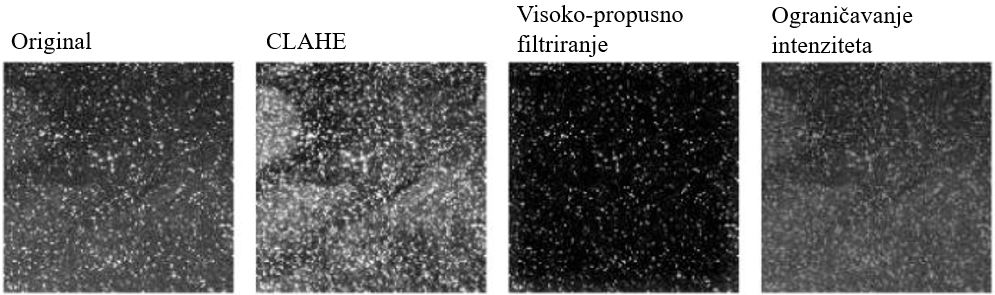
\includegraphics[width=16.5cm]{./2_DPIV/2_5IzostravnjeSlike.jpg} 
	\caption{Primjer dobivenog efekta nakon primjene u tekstu opisanih pretprocesorskih tehnika \cite{thielicke2014_article}}
	\label{sl:2.5}
\end{figure}
\FloatBarrier
\subsection{Ograničavanje intenziteta}
Čest izvor grešaka u DPIV analizi je prisutnost jako svijetlih mrlji unutar PIV slika \cite{shavit2007intensity}. Svijetle mrlje su okarakterizirane intenzitetom sivih tonova mnogo većim od srednje vrijednosti intenziteta slike. Pomak svijetlih mrlja u odnosu na ostale čestice više pridonosi korelacijskom signalu unutar područja ispitivanja, što dovodi do veće pristranosti u konačnom vektoru brzina. \textit{Ograničavanje intenziteta} (\textit{eng. Intensity Capping}) je tehnika poboljšanja slike koja daje bolje PIV rezultate u slučaju da se na slici nalaze svijetle mrlje. Tehnikom ograničavanja intenziteta korisniku je omogućeno određivanje gornje granice intenziteta sivih tonova u području ispitivanja. Svi pixeli koji premaše zadani prag zamijene se iznosom gornje granice. Računanje pomaka u tom slučaju bolje predstavlja pomak svih čestica u području ispitivanja, a pristranost prema svijetlim mrljama je minimizirana. Ograničavanje intenziteta poboljšava detekciju ispravnih vektora brzina za $5.2 \pm 2.5\%$. Na \textit{Slici \ref{sl:2.6}a} prikazana je originalna PIV fotografija sa svojim rezultirajućim poljem brzina (dolje), te PIV slika nakon primjene ograničavanja intenziteta (\textit{Slika \ref{sl:2.6}b}) sa poljem brzina, također. Sa slika je vidljivo kako primjena ograničavanja intenziteta je mnogo utjecala na pojavu individualnih pristranih vektora brzina (Napomena - na slikama su prikazani samo dijelovi cijele domene radi estetskih razloga, pa zbog toga same slike i rezultati nisu u mjerilu).
\begin{figure}[h]  
	\centering
	%\usepackage{graphicx}
	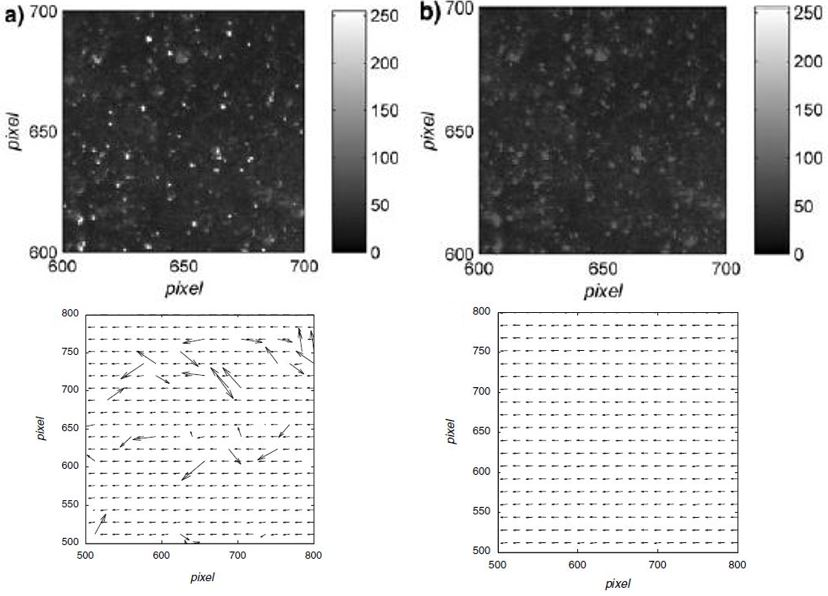
\includegraphics[width=11cm]{./2_DPIV/2_6IntensityCapping.jpg} 
	\caption{Primjer primjene tehnike ograničavanja intenziteta, te dobivena polja brzina nakon analize kros-korelacijom \cite{shavit2007intensity}}
	\label{sl:2.6}
\end{figure}
\FloatBarrier
\section{Evaluacija slike}
Najosjetljiviji i najvažniji dio efikasnosti i točnosti DPIV analize je sama kros-korelacija PIV fotografija. Korelacija je bilo koji statistički odnos, te predstavlja međusobnu povezanost između različitih pojava predstavljenih vrijednostima dviju varijabli. Pri tome povezanost znači da je vrijednost jedne varijable moguće sa određenom vjerojatnošću predvidjeti na osnovi saznanja o vrijednosti druge varijable \cite{wiki:Correlation}. U 1D obradi signala kros-korelacija je mjera sličnosti dviju serija kao funkcija relativnog pomaka jedne serije u odnosu na drugu seriju, što je poznato kao i "\textit{klizajući skalarni produkt}" (\textit{eng. sliding dot product} ili \textit{sliding inner-product}). Glavni cilj kros-korelacije u DPIV analizi je evaluacija PIV fotografija kako bi se odredio pomak između dva lokalna uzorka nasumično distribuiranih čestica, koje su spremljene kao 2D distribucija sivih tonova. Teoriju 1D kros korelacije iz obrade signala lako je proširiti na 2D (npr. ravninska distribucija sivih tonova) ili 3D (prostorna distribucija) \cite{raffel2018_book}.
\par
Kao što je već spomenuto ranije prvi korak DPIV evaluacije je podijeliti PIV snimke na manja područja (prozore) ispitivanja (\textit{eng. interrogation areas (windows)}). Prozor ispitivanja predstavlja lokalni uzorak čestica PIV fotografije koji je opisan jednim vektorom brzine, pa prema tome veličina prozora ispitivanja određuje do koje razine rezolucije je dobiveno polje brzina.
\par
Neka se sada pretpostavi kako su snimljene dvije uzastopne PIV snimke iz stroboskopom osvijetljene svjetlosne ravnine (za početak neka budu zanemareni efekti kašnjenja čestica, 3D gibanja,...). Iz dvije uzastopne snimke sve što je moguće izmjeriti je pravocrtni pomak u vremenu (za dobivanje informacija o ubrzanju i zakrivljenosti strujanja, potrebno je više snimki). Ove dvije snimke (\textit{Slika \ref{sl:2.7}}) mogu dati vektor pravocrtnog pomaka, gdje je svaki vektor formiran iz analize gibanja lokalnog uzorka čestica iz prozora ispitivanja.
\begin{figure}[h]  
	\centering
	%\usepackage{graphicx}
	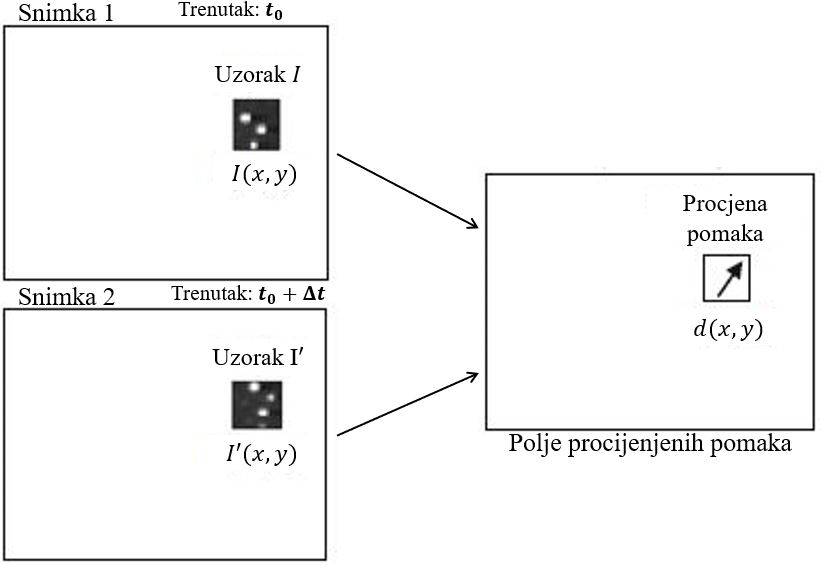
\includegraphics[width=11cm]{./2_DPIV/2_7OpisGibanja.jpg} 
	\caption{Konceptualni prikaz povezivanja kadrova snimki 1 i 2 i dobivanja vektora pomaka\cite{raffel2018_book}}
	\label{sl:2.7}
\end{figure}
\par
U suštini kros-korelacija je tehnika statističkog povezivanja uzorka iz snimke 1 (snimljene u trenutku $t_0$) sa uzorkom iz snimke 2 (snimljene u trenutku $t_0 + \Delta{t}$). Ova statistička tehnika implementirana je uz pomoć funkcije diskretne kros-korelacije \cite{raffel2018_book}:
\begin{equation}
	R_{II}(x, y) = \sum_{i=-M}^{M}\sum_{j=-N}^{N}I(i, j)I'(i+x, j+y)
	\label{eqn:2.4}
\end{equation}
gdje su varijable $I$ i $I'$ odgovarajući prozori ispitivanja (vrijednosti intenziteta) iz slika (ekspozicija) 1 i 2. Za dani pomak diskretna kros-korelacija stoga mjeri "poklapanje" prozora ispitivanja $I$ sa prozorom $I'$. Lokacija najvećeg vrha intenziteta (najveća vrijednost) u rezultirajućoj korelacijskoj matrici $R_{II}$ daje najvjerojatniji mogući pomak čestica iz snimke 1 u snimku 2.
\par
Jednadžba \ref{eqn:2.4} rješava se na dva načina. Najizravniji pristup je da se korelacijska matrica izračuna u prostornoj domeni, ovaj pristup naziva se direktna kros-korelacija (ili konvolucijsko filtriranje). Drugi pristup dobivanja korelacijske matrice je računanje u frekvencijskoj domeni (diskretna Fourier-ova transformacija - DFT). DFT se računa koristeći FFT algoritam (\textit{eng. Fast Fourier Transform}) i u principu je brži način dobivanja korelacijske matrice, za razliku od direktnog računanja koje je sigurnije i točnije.
\FloatBarrier
\subsection{Direktna prostorna kros-korelacija}
Direktna kros-korelacija (DKK) računa korelacijsku matricu u prostornoj domeni. U DKK , prozori ispitivanja $I$ i $I'$ obično su različitih veličina. Ako se odabere da je područje $I'$ bude duplo veće od područja $I$, pomicanje čestica do polovine veličine $I$ neće rezultirati gubitkom podataka i pružit će pouzdanu matricu korelacije sa niskim pozadinskim šumom (\textit{Slika \ref{sl:2.8}}).
\begin{figure}[h]  
	\centering
	%\usepackage{graphicx}
	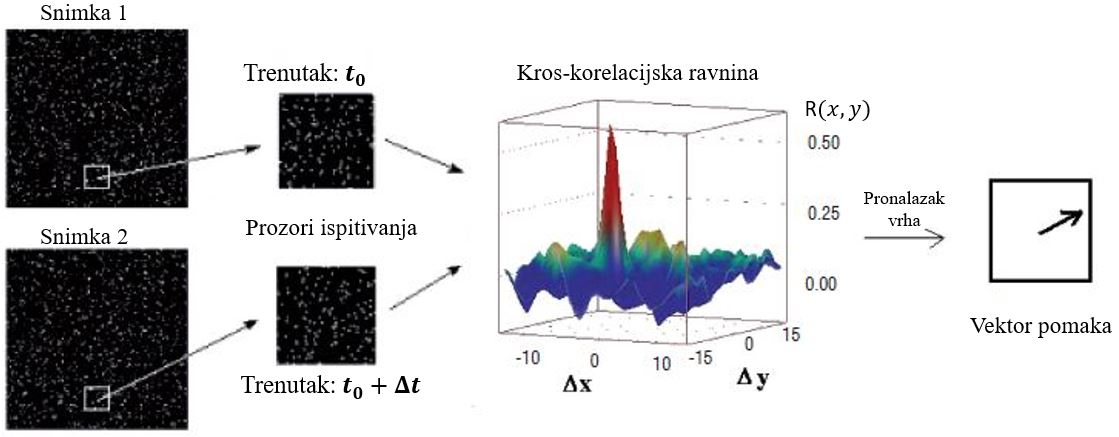
\includegraphics[width=14cm]{./2_DPIV/2_8KrosKorelacijskaRavnina.jpg} 
	\caption{Konceptualni prikaz povezivanja kadrova snimki 1 i 2 i dobivanja vektora pomaka\cite{brossard2009_article}}
	\label{sl:2.8}
\end{figure}
\par
Direktna kros-korelacija prozor ispitivanja $I$ iz jednadžbe \ref{eqn:2.4} linearno "pomiče" oko prozora $I'$ bez da prijeđe preko ruba $I'$. Za svaki odabir pomaka uzorka $(x, y)$, dobije se vrijednost intenziteta kros-korelacije $R_{II}(x, y)$, što je u suštini suma umnožaka intenziteta svih pixela koji se preklapaju. Ako se ova operacija izvede na rasponu pomaka ($-M \leq x \leq M$; $-N \leq y \leq N$), dobije se kros-korelacijska ravnina veličine $(2M+1) \times (2N+1)$. Ovaj postupak pomicanja grafički je prikazan na \textit{Slici \ref{sl:2.9}}, gdje je dan primjer sa $4 \times 4$ prozorom $I$ koji je koreliran sa $8 \times 8$ prozorom $I'$ koji skupa formiraju $9 \times 9$ korelacijsku matricu $R$. 
\begin{figure}[h]  
	\centering
	%\usepackage{graphicx}
	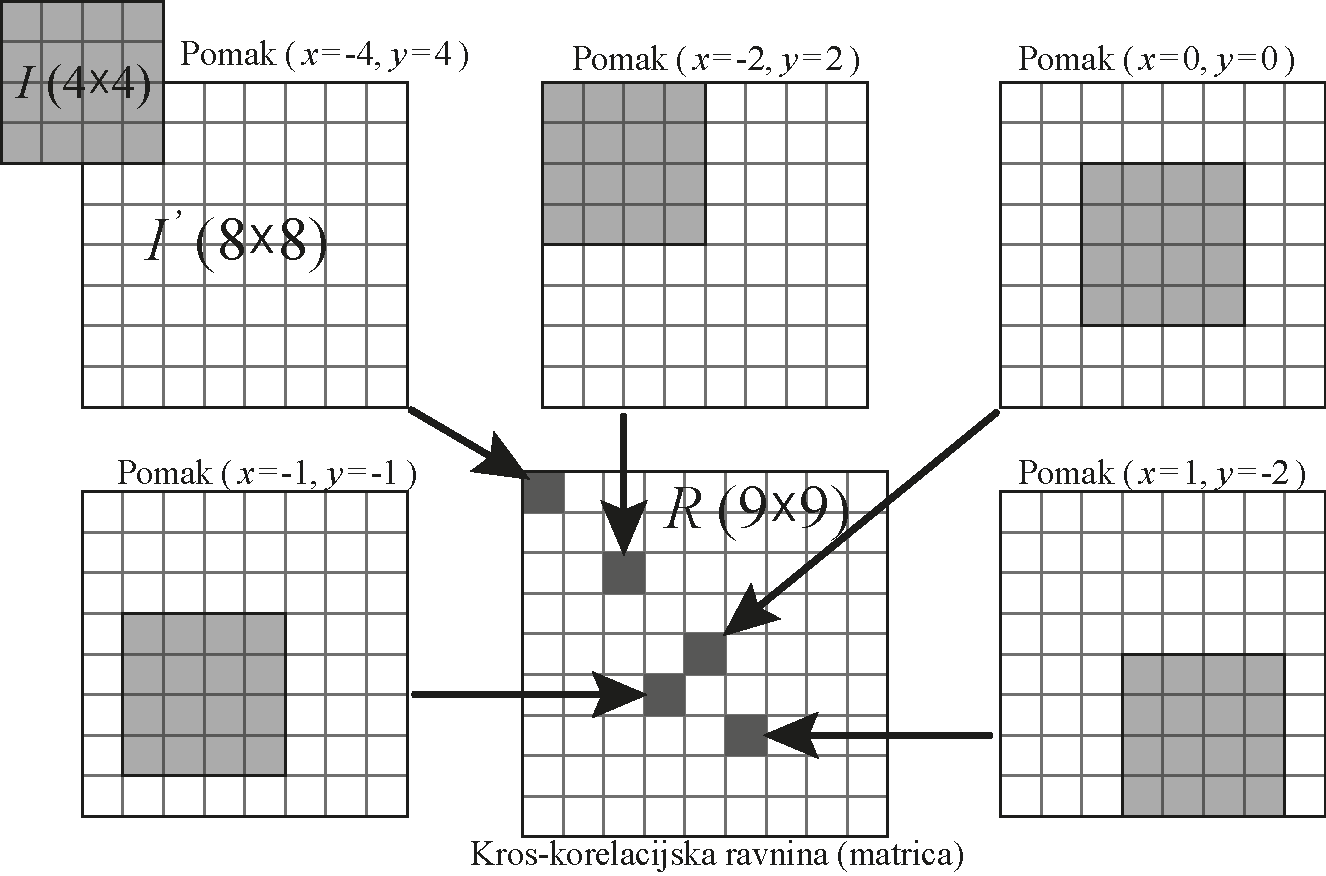
\includegraphics[width=16cm]{./2_DPIV/2_9PostupakPomicanja.pdf} 
	\caption{Primjer formacije korelacijske ravnine koristeći DKK}
	\label{sl:2.9}
\end{figure}
\par
Za vrijednosti pomaka gdje se prozor ispitivanja $I$ poklopi sa prozorom $I'$ suma umnožaka intenziteta pixela imat će najveću vrijednost, te će ta vrijednost signalizirati pomak čestica. Ukratko, kros-korelacijska funkcija (jednadžba \ref{eqn:2.4}) statistički mjeri stupanj preklapanja između dva prozora ispitivanja za dani pomak. U današnjim PIV evaluacijama tipične veličine prozora ispitivanja su $32 \times 32$ pixela (ili $16 \times 16$ pixela).
\par
Iz implementacije DKK mogu se uočiti dva nedostatka \cite{raffel2018_book}. 
\begin{itemize}[topsep=0pt, itemsep=0em]
	\item Prvo, broj računanja po korelaciji eksponencijalno (kvadratno) raste  sa povećanjem prozora ispitivanja. Tipična PIV analiza koristi nekoliko tisuća pixela, dok je raspon ispitivanja oko $\pm 20$ pixela, što znači da se mora izvršiti preko milijun multiplikacija i zbrajanja kako bi se formirala samo jedna korelacijska matrica. Ako se uzme u obzira da se mora izračunati nekoliko tisuća vektora pomaka računalna snaga počinje igrati veliku ulogu u računanju korelacijske matrice. Jedan od načina zaobilaska problema kvadratnog rasta računanja je korištenje Fourier-ove transformacije i računanja u frekvencijskoj domeni, što je i objašnjeno u daljnjem radu. No ipak u zadnje vrijeme dolazi do razvoja računalne tehnologije i tehnike paralelnog računanja na grafičkim jedinicama (GPU) što značajno pridonose brzini kalkulacija, te potencijalno čini DKK dovoljno brzim za primjenu.
	\item Drugo, kros-korelacijskom metodom dobiju se samo pravocrtni pomaci - \textit{metoda prvog stupnja} (\textit{eng. first order method}), što znači da je ne moguće izvući informacije o rotacijama i deformacijama. Ovo znači da se veličina prozora ispitivanja mora odabrati dovoljno malenom da se može smatrati kako su efekti višeg stupnja (rotacija, deformacija) zanemarivi.
\end{itemize}
\FloatBarrier
\subsection{Računanje korelacijske funkcije u frekvencijskoj domeni}
Glavni problem direktnom računanju korelacijske matrice (potrebna računalna snaga) može se riješiti tako da se korelacijska matrica izračuna u frekvencijskoj domeni koristeći diskretnu Fourier-ovu transformaciju (DFT). Na taj način bi se iskoristila prednost  korelacijskog teorema koji tvrdi da kros-korelacija dviju funkcija je ekvivalentna kompleksno-konjugiranom umnošku njihove Fourier-ove transformacije:
\begin{equation}
	R_{II} \iff \hat{I}\cdot \hat{I}'^*
	\label{eqn:2.5}
\end{equation}
gdje su $\hat{I}$ i $\hat{I}'$ Fourier-ove transformacije funkcija $I$ i $I'$. U praksi
Fourier-ova transformacija za diskretne podatke se efikasno računa koristeći FFT (\textit{eng. fast Fourier transform}) algoritam koji smanjuje računanje sa $O[N^2]$ operacija na $O[N\log N]$ operacija. Tako se zahtjevni 2-dimenzionalni korelacijski proces može svesti na računanje 2D FFT-ova jednako velikih uzoraka ispitivanja sa snimke nakon čega slijedi kompleksno-konjugirano množenje rezultirajućih Fourier-ovih koeficijenata. Dobiveni koeficijenti se onda inverznom Fourier-ovom transformacijom vrate u prostornu domenu (kros-korelacijsku ravninu) koja ima istu prostornu dimenziju kao i ulazne slike 1 i 2 (\textit{Slika \ref{sl:2.10}}).
\begin{figure}[h]  
	\centering
	%\usepackage{graphicx}
	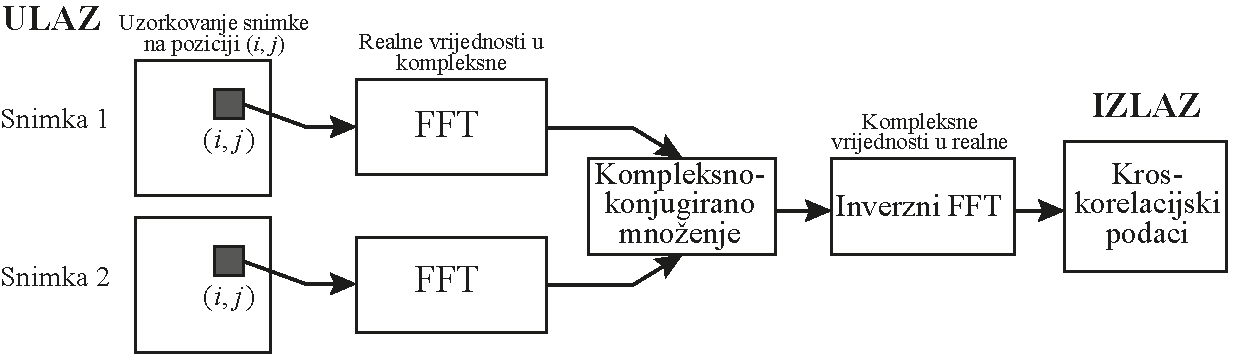
\includegraphics[width=16.5cm]{./2_DPIV/2_10FFT_postupak.pdf} 
	\caption{Računanje kros-korelacije koristeći FFT \cite{raffel2018_book}}
	\label{sl:2.10}
\end{figure}
\par
DFT pristup koristi prozore ispitivanja iz snimki 1 i 2 koji su iste veličine što rezultira određenim gubitkom informacija, koji se registrira pojavom pozadinskog šuma u korelacijskoj matrici \cite{thielicke2014_article}. Pozadinski šum u korelacijskoj ravnini komplicira detekciju vrhova, što smanjuje točnost mjerenja. Dodatni problem korištenja DFT je to što FFT po definiciji pretpostavlja da su ulazni podaci (prozori ispitivanja) periodični, to jest da se ponavljaju u svim smjerovima. Ako je pomak čestica veći od polovice veličine prozora ispitivanja, vrh u korelacijskoj ravnini je "presavijen" u matrici, te se pojavi na suprotnoj strani korelacijske ravnine. Za točni pomak $d_{x,to\textup{č}no}>N/2$, izmjereni pomak će iznositi $d_{x,izmjereno}=d_{x,to\textup{č}no}-N$. U tom slučaju kriterij uzorkovanja (Nyquist-Shanon-ov teorem) neće biti ispunjen što dovodi do pod-uzorkovanja podataka (\textit{eng. aliasing}). Stoga, pomak čestica obavezno mora biti manji od polovice veličine prozora ispitivanja. Preporuka je da pomak bude jedna četvrtina veličine prozora ispitivanja (\textit{eng. one-quarter rule}), kako bi se pozadinski šum u korelacijskoj matrici održao na niskim razinama. Još jedan način na koji se pozadinski šum može minimizirati, uz povećanje prozora ispitivanja je da se smanji vrijeme između snimki kamere. Također moguće je da se provode više prolaza diskretne Fourier-ove transformacije (DFT) na isti set podataka (prozora ispitivanja), što značajno povećava omjer signal-šuma \cite{thielicke2014_article}. Nakon prve DFT analize (prvog prolaza), dobivena cjelobrojna vrijednost se koristi kao podatak koji će promijeniti veličinu prozora ispitivanja u sljedećem prolazu, te tako minimizirati gubitak informacija zbog pomaka čestica. Nadalje, kako bi se dodatno poboljšao DFT  algoritam moguće je poboljšati mrežu ispitivanja sa svakim prolazom. Prvi prolaz bi koristio veće prozore ispitivanja te bi tako pronašao i veće pomake čestica. U sljedećim prozorima, prozori ispitivanja bi se smanjili i pomakli u isto vrijeme što bi dovelo do veće prostorne rezolucije, te većeg raspona mjerenih brzina.
\par
Još jedna negativna strana periodičnosti korelacijskih podataka je u tome da korelacijske procjene budu pristrane. Sa sve većim pomacima, sve se manje podataka međusobno korelira budući da periodički kontinuirani podaci korelacijskog uzorka ne daju nikakav doprinos korelacijskoj vrijednosti. Vrijednosti na rubu korelacijske ravnine računaju se samo iz preklapajuće polovice podataka i treba ih ispravno ponderirati. Ukoliko podaci nisu ispravno ponderirani, procjena pomaka biti će pristranija nižoj vrijednosti (\textit{Slika \ref{sl:2.11}}). Snimke sa većim česticama daju šire korelacijske vrhove, te samim time i veće greške pristranosti. U poglavlju koje opisuje detekciju korelacijskih vrhova ukratko je opisana pogodna funkcija kojom je moguće rješavanje problema pristrane pogreške
\begin{figure}[h]  
	\centering
	%\usepackage{graphicx}
	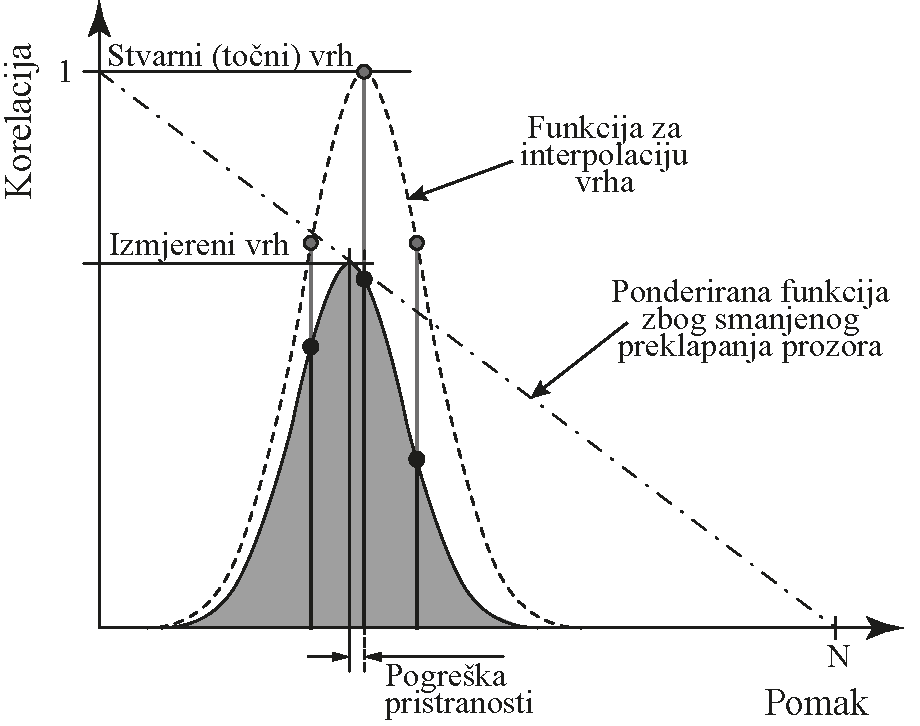
\includegraphics[width=10cm]{./2_DPIV/2_11BiasError.pdf} 
	\caption{Pogreška pristranosti u računanju kros-korelacije koristeći FFT \cite{raffel2018_book}}
	\label{sl:2.11}
\end{figure}
\par
Do sada je pretpostavljeno kako čestice unutar prozora ispitivanja imaju uniformno gibanje. U stvarnom strujanju čestice su podvrgnute raznim smicanjima i rotacijama, što dovodi do ne-uniformnog gibanja koje proširuje intenzitete vrhova u korelacijskoj ravnini, te rezultira lošijim rezultatima. Postoji nekoliko tehnika koje uzimaju u obzir transformaciju prozora ispitivanja (višestruki prolaz, poboljšanje mreže prozora, \textit{tehnika deformacije prozora}). U PIVlab softveru se primjenjuje sljedeći postupak: Analiza započinje sa standardnim DFT algoritmom. Prvi prolaz DFT-a daje informacije o pomaku centra svakog prozora ispitivanja. Kada dođe do preklapanja područja jedno preko drugo za npr. 50\% dobije se dodatna informacija o pomaku na granicama i uglovima svih područja ispitivanja (sveukupno devet pozicija, \textit{Slika \ref{Tehnika deformacije prozora} lijevo}). Uz pomoć dobivene informacije izračuna se pomak svakog pixela unutar prozora ispitivanja koristeći bilinearnu interpolaciju. Nakon toga, područje ispitivanja B se deformira prema dobivenom pomaku (\textit{Slika \ref{Tehnika deformacije prozora} desno}) koristeći bilinearnu interpolaciju ili spline interpolaciju (preciznije, ali sporije). Sljedeći prolaz ispitivanja korelira originalno područje A sa deformiranim područjem B. Akumuliraju se preostale informacije o pomaku prilikom svakog prolaza. Nakon nekoliko prolaza, deformirano područje ispitivanja B izgleda gotovo identično kao originalno područje A, te je pomak određen sa velikom preciznošću. Između prolaza, ali ne nakon posljednjeg prolaza, informacije o brzini su izglađene i potvrđene, a informacije koje nedostaju su interpolirane.
\begin{figure}[h]  
	\centering
	%\usepackage{graphicx}
	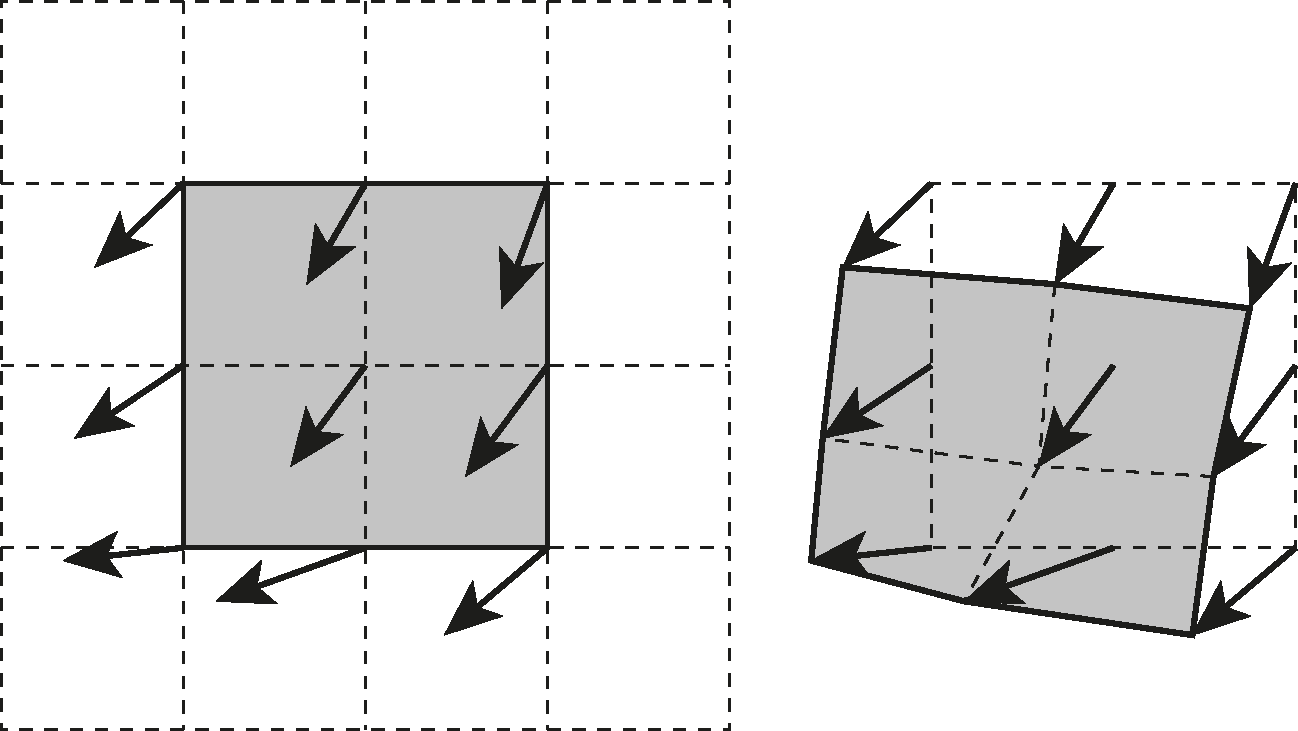
\includegraphics[width=8cm]{./2_DPIV/TehnikaDeformacijeProzora.pdf} 
	\caption{Princip tehnike deformacije prozora, na lijevoj slici se nakon prvog prolaza dobije informacija o pomaku koja je vidljiva na 9 lokacija. Informacije o pomacima se nakon toga interpoliraju kako bi se dobio pomak svakog pixela prozora ispitivanja, te konačno imamo novi prozor ispitivanja koji će se koristiti u sljedećem prolazu DFT-a \cite{thielicke2014_phd}}
	\label{Tehnika deformacije prozora}
\end{figure}
\FloatBarrier
\subsection{Računanje korelacijskog koeficijenta}
U brojnim slučajevima korisno je kvantificirati stupanj korelacije između dva uzorka prozora ispitivanja. Standardna kros-korelacijska funkcija (jednadžba \ref{eqn:2.4}) daje različite vrijednosti maksimalnih korelacija za isti stupanj poklapanja, zbog toga što kros-korelacijska funkcija nije normalizirana. Na primjer, prozori ispitivanja sa mnogo (svijetlih) čestica daju mnogo veću vrijednost korelacijskog koeficijenta od uzoraka gdje su čestice manje svijetle. Na ovaj način usporedba stupnja korelacije između individualnih prozora ispitivanja nije moguća. Funkcija kros-korelacijskog koeficijenta (\ref{eqn:2.6}) normalizira kros-korelacijsku funkciju (\ref{eqn:2.4}) na način:
\begin{subequations} \label{eqn:2.6}
	\begin{equation}
		c_{II}(x, y)=\frac{C_{II}(x, y)}{\sqrt{\sigma_{I}(x, y)}\sqrt{\sigma_{I'}(x, y)}} \tag{\ref{eqn:2.6}}
	\end{equation}
gdje su:
	\begin{align}
		\begin{split} \label{eqn:2.6a}
			C_{II}(x, y) &= \sum_{i=0}^{M}\sum_{j=0}^{N}\left[ I(i, j)-\mu_{I}\right]\left[ I'(i+x, j+y)-\mu_{I'}(x, y)\right]
		\end{split} \\
		\begin{split} \label{eqn:2.6b}
			\sigma_{I}(x, y) &= \sum_{i=0}^{M}\sum_{j=0}^{N}\left[I(i, j)-\mu_{I}\right]^{2}
		\end{split} \\
		\begin{split} \label{eqn:2.6c}
			\sigma_{I'}(x, y) &= \sum_{i=0}^{M}\sum_{j=0}^{N}\left[I'(i, j)-\mu_{I'}(x, y)\right]^{2}
		\end{split}
	\end{align}
\end{subequations}
Vrijednost $\mu_{I}$ je prosjek predloška prozora i računa se samo jednom, dok $\mu_{I'}(x, y)$ je prosjek $I'$ koji se podudara predloškom prozora $I$ na poziciji $(x, y)$. $I'$ mora se izračunati na svakoj poziciji $(x, y)$. Jednadžbu \ref{eqn:2.6} značajno je teže implementirati koristeći FFT algoritam i obično se računa direktno u prostornoj domeni. Unatoč računalnoj kompleksnosti, jednadžba dopušta da uzorci (prozori) budu nejednake veličine što može biti vrlo korisno u podudaranju malih grupa čestica. Ipak aproksimacija prvog reda pravilnoj normalizaciji je moguća ako su prozori ispitivanja jednake veličine i nisu obloženi nulama. 
\begin{enumerate}[label=\textbf{Korak \arabic*:}, leftmargin=*, align=left, topsep=0pt, itemsep=0em]
	\item Uzrokovati prozore ispitivanja na željenim lokacijama, te izračunati srednju i standardnu devijaciju svake slike
	\item Oduzeti srednju vrijednost od svakog uzorka
	\item Izračunati kros-korelacijsku funkciju koristeći 2D FFT-ove (kao što je prikazano na slici \ref{sl:2.10})
	\item Podijeliti kros-korelacijske vrijednosti sa standardnom devijacijom originalnog uzorka. Zbog postupka normalizacije rezultirajuće vrijednosti će upasti u raspon $-1\leq c\leq 1$.
	\item Nastaviti sa detekcijom korelacijskog vrha uzimajući u obzir sve (ne)mogućnosti FFT kros-korelacije.
\end{enumerate}
\subsection{Pronalazak korelacijskog vrha}
Još jedan veoma bitan faktor pri PIV analizi koji izravno utječe na točnost mjerenja je odabir tehnike pronalaska korelacijskog vrha. Cjelobrojni pomak dva prozora ispitivanja može biti izravno određen iz lokacije najvećeg vrha korelacije korelacijske matrice \cite{thielicke2014_article}. No, lokacija nadalje može biti određena i sub-pixelskom preciznošću koristeći razne metode.
\par
Kako su ulazni podaci u PIV analizi diskretizirani, vrijednosti korelacije postoje samo za integralne pomake. Najveća vrijednost korelacije tada bi omogućila određivanje pomaka sa nesigurnošću od $\pm \, 1/2$ pixela. Međutim, kako je kros-korelacijska funkcija statistička mjera najboljeg poklapanja, korelacije vrijednosti oko vrha također sadrže korisne informacije \cite{raffel2018_book}. Na primjer, ako ispitivani uzorak sadrži $10$ parova čestica koje su dale procijenjeni pomak koji u prosjeku malo varira sa vrijednosti od $2.5$ pixela, statistički bi to značilo da je $5$ parova čestica dalo pomak od $3$ pixela, a preostalih $5$ parova pomak od $2$ pixela. Iz ovog grubog primjera, jasno je kako se informacije skrivene u vrijednostima korelacije mogu iskoristiti za procjenu srednjeg pomaka slike unutar prozora ispitivanja.
\par
U literaturi \cite{raffel2018_book} opisane su razne metode procjene lokacije korelacijskog vrha. Jedan od robustnijih načina procjene lokacije je taj da se korelacijski podaci aproksimiraju sa određenom funkcijom. Ova metoda je posebno dobra kod uskih korelacijskih vrhova, pošto se ovim pristupom uobičajeno koriste samo 3 susjedne vrijednosti korelacijske matrice (u x ili y smjeru). Najčešće korištena je aproksimacija vrha korelacije Gauss-ovom funkcijom. 
\begin{equation}
	f(x)=C\exp \left[\dfrac{-(x_{0}-x)^{2}}{k}\right]
	\label{eqn:2.7}
\end{equation}
Korištenje Gauss-ove funkcije za aproksimaciju je najprikladnije iz razloga što individualne snimke čestica usko se podudaraju sa Gauss-ovom distribucijom intenziteta (imaju oblik Airy-eve funkcije intenziteta - \textit{Slika \ref{sl:3.2}}), te kros-korelacija dvije Gauss-ove distribucije ponovno daje korelacijsku matrica sa Gauss-ovom distribucijom.
\par
Kada je poznata najveća vrijednost vrha korelacije u korelacijskoj matrici, pomoću ostalih podataka iz matrice Gauss-ovom funkcijom moguće je točnije (sub-pixelski) aproksimirati vrh korelacije (\textit{Slika \ref{sl:2.12}}). Dovoljna je upotreba samo neposredno susjednih vertikalnih i horizontalnih pixela, te je moguće evaluirati x i y os odvojeno. Implementacija aproksimacije u 3 točke se vrši na način:
\begin{figure}[h]  
	\centering
	%\usepackage{graphicx}
	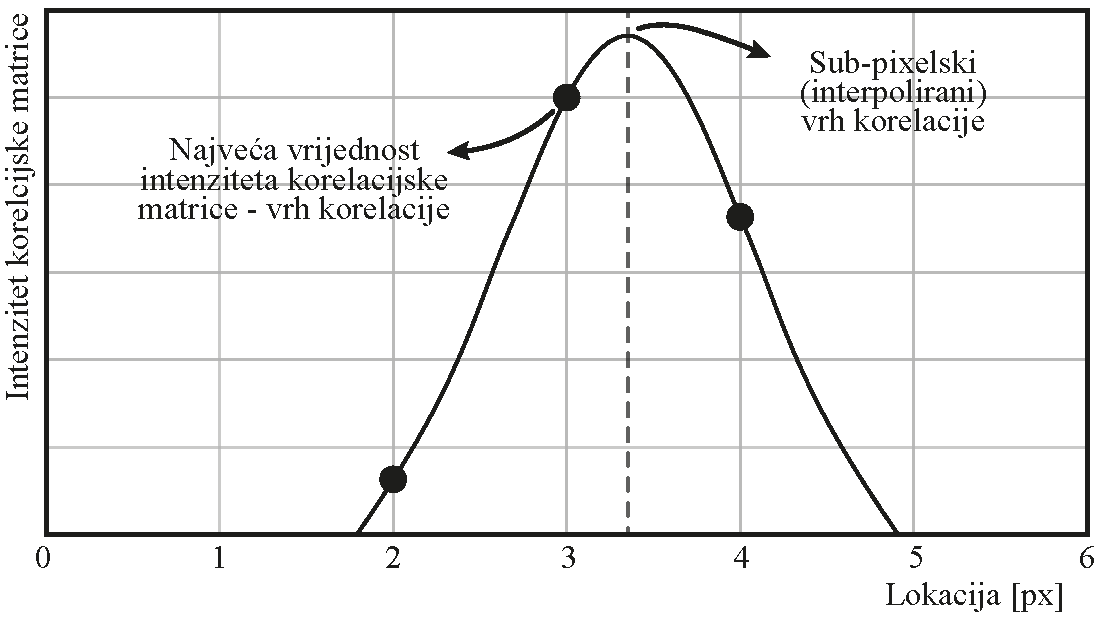
\includegraphics[width=11cm]{./2_DPIV/2_12DetekcijaVrha.pdf} 
	\caption{Princip aproksimacije u 3 točke Gauss-ovom funkcijom, točke predstavljaju vrijednosti intenziteta korelacijske matrice za samo jednu os}
	\label{sl:2.12}
\end{figure}
\begin{enumerate}[label=\textbf{Korak \arabic*:}, leftmargin=*, align=left, topsep=0pt, itemsep=0em]
	\item Pronaći maksimalne korelacijske vrijednosti $R(i, j)$ u korelacijsku ravninu $R_{II}$, te zapamtiti njihove $(i, j)$ koordinate.
	\item Izvući četiri susjedne korelacijske vrijednosti: $R_{(i-1,j)}$, $R_{(i+1,j)}$, $R_{(i,j-1)}$ i $R_{(i,j+1)}$
	\item Koristeći tri točke u svakom smjeru osi, provući Gauss-ovu krivulju gdje su $C$, $x_{0}$ i $k$ koeficijenti koje treba dobiti nekom od metoda interpolacije (npr. nelinearna regresija iz jednadžbe \ref{eqn:2.7})
\end{enumerate}
Potrebno je napomenuti u slučaju da je pomak čestica unutar prozora ispitivanja podvrgnut smicanju ili rotaciju ili su snimke previše mutne tada korelacijski vrh ima ne-simetričan (eliptičan) oblik, te korištenje aproksimacije u jednom smjeru sa 3 vrijednosti Gauss-ovom funkcijom može izazvati pogreške. Ovaj efekt se može izbjeći ako se koristi 2D aproksimacija Gauss-ovom funkcijom (fittanje u 9 točaka).
\begin{equation}
	f(x, y)=I_{0}\, \exp \left[\dfrac{-(x-x_{0})^{2}}{(1/8)d_{\tau x}^{2}}-\dfrac{-(y-y_{0})^{2}}{(1/8)d_{\tau y}^{2}}-\dfrac{k_{xy}(x-x_{0})(y-y_{0})}{d_{\tau x}d_{\tau y}}\right]
	\label{eqn:2.8}
\end{equation}
Jednadžba \ref{eqn:2.8} sadrži ukupno 6 koeficijenata koje je potrebno dobiti (naprimjer ponovno nekom regresijskom metodom). Koeficijenti $d_{\tau x}$ i $d_{\tau y}$ predstavljaju širine korelacijskih vrhova u $x$ i $y$ smjeru, dok koeficijent $k_{xy}$ predstavlja "eliptičnost" korelacijskog vrha. Maksimalni iznos vrha korelacije $I_{0}$ određen je pozicijom $x_{0}$ i $y_{0}$.
\FloatBarrier
\section{Postprocesiranje PIV podataka}
Iako napredni kros-korelacijski algoritam pruža dosta robusnu procjenu brzine unutar područja ispitivanja, i dalje mnogi faktori (loše osvjetljenje, jako 3D strujanje,...) uzrokuju nepravilnu korelaciju koju je do određene mjere naknadno moguće ispraviti koristeći razne tehnike obrade dobivenih PIV rezultata. U principu, post-procesiranje PIV podataka sastoji se od sljedećih koraka:
\begin{description}[style=unboxed,leftmargin=0cm]
	\item[Provjera valjanosti neobrađenih (\textit{eng. raw}) podataka.] Nakon automatske evaluacije PIV snimki, određeni broj očito nepravilno određenih vektora brzina koji se na engleskom nazivaju "\textit{outliers}" ("\textit{vrijednosti koje strše}") obično se može prepoznati vizualnom inspekcijom neobrađenih podataka. U svrhu da se odrede nepravilni vektori ovaj post-proces prepoznavanja pogrešnih vektora mora biti automatiziran. Potrebno je napomenuti kako je provjera valjanosti podataka prvi i najvažniji korak, jer utječe na kvalitetu provedbe svih ostalih tehnika postprocesiranja PIV podataka.
	\item[Zamjena pogrešnih podataka.] Kod većine post-proces algoritama potrebno je imati kompletno popunjena polja podataka u Kartezijevoj mreži, što je i slučaj kod numeričkih simulacija. Ako se dogodi da nedostaje jedan podatak u mreži, taj podatak je potrebno aproksimirati sa određenom vrijednosti brzine.
	\item[Smanjenje podataka.] Često je komplicirano pratiti nekoliko tisuća podataka o brzinama i pomacima, pogotovo u slučaju 3D PIV analize i dugotrajnih strujanja. Usrednjavanje podataka u ovim slučajevima je poprilično jednostavna tehnika. U slučaju da je uzorkovanje strujanja više-manje uvjetovano, te tada treba razlikovati periodične i ne-periodične fluktuacije u strujanju, smanjivanje podataka usrednjavanjem više nije tako jednostavno. Također moguće je podatke o strujanju pojednostavniti uz pomoć operatora za vektorsko polje (npr. korištenje rotacije i divergencije brzine). Nadalje u novije vrijeme evaluacija nestacionarnih strujanja zahtjeva pojednostavljenja koja se izvršavaju preko dekompozicijskih tehnika. Najčešće korištene dekompozicijske tehnike u ovom slučaju su: \textit{pravilna ortogonalna dekompozicija} (POD) (\textit{eng. Proper Orthogonal Decomposition}) poznata kao i \textit{analiza glavnih komponenti} (PCA) (\textit{eng. Principal Component Analysis}), te \textit{dinamička modalna dekompozicija} (DMD) (\textit{eng. Dynamic Mode Decomposition}).
	\item[Asimilacija podataka] Često kada se provode PIV eksperimenti, dosta stvari o promatranoj vrsti strujanja je poznato i analitički određeno, pogotovo za slučajeve elementarnih tipova strujanja. U tom slučaju PIV podatke je moguće obraditi na takav način da lokalno ispunjavaju matematičke zakone.
\end{description}
\subsection{Provjera valjanosti podataka}
Kako je broj nepravilnih vektora brzina znatan, čak i ako se koriste najnaprednije korelacijske metode. Potrebno je korištenje (polu)automatske provjere valjanosti podataka (\textit{eng. Data Validation}) kako bi se učinkovito suzbili pogrešni podaci. U literaturama postoji mnogo metoda i algoritama za provjeru valjanosti podataka, te treba napomenuti kako nijedna od tih tehnika nije generalno dobra za sve PIV analize. No, ipak u ovom radu će biti opisane neke od najkorištenijih metoda provjere valjanosti podataka, koje su i implementirane u korišteni softver.
\par
Prije samog opisa validacijskih algoritama, potrebno je definirati varijable i izraze koji će se koristiti u daljnjem tekstu \cite{raffel2018_book}. Neka je trenutno polje brzina $(U, V)$ uzorkovano ("ispitano") na lokacijama koje formiraju strukturiranu mrežu u polju strujanja.  U ovom slučaju mreža  je prikazana na \textit{Slici \ref{sl:2.13}} i sastoji se od $I\times J$ čvorova, međusobno udaljenih u $X$ i $Y$ smjeru za $\Delta X$ i $\Delta Y$. U svakom čvoru $i, j \, (i=1,\dots ,I;\, j=,\dots ,J)$ opisana je brzina $\boldsymbol{U}_{2D}(i, j)$. U ovom slučaju bitna je veza između $\boldsymbol{U}_{2D}(i, j)$ i njegovih najbližih susjeda koji su označeni sa $\boldsymbol{U}_{2D}(n)$ gdje $n$ ide $n \, (n=1,\dots,N)$, a $N$ označava broj susjeda kojih je uobičajeno osam. Sada je potrebno definirati vrijednost razlike vektora između središnjeg vektora $\boldsymbol{U}_{2D}(i, j)$, te susjednih vektora $\boldsymbol{U}_{2D}(n)$:
\begin{equation}
	|\boldsymbol{U}_{\Delta , n}|=|\boldsymbol{U}_{2D}(n)-\boldsymbol{U}_{2D}(i,j)|
	\label{eqn:2.9}
\end{equation}
\begin{figure}[h]  
	\centering
	%\usepackage{graphicx}
	\includegraphics[width=12cm]{./2_DPIV/2_13MeshPostProc.pdf} 
	\caption{Shema mreže podataka sa označenim vektorima}
	\label{sl:2.13}
\end{figure}
\begin{description}[style=unboxed,leftmargin=0cm]
	\item[Provjera razlike vektora] Jednostavna tehnika za suzbijanje nepravilnih vektora je definiranje granice vrijednosti komponenti vektora brzina za određeno područje, tvz. gradijent filtar. Gradijent filtar se računa uz pomoć izraza \ref{eqn:2.9}. Ideja korištenja gradijent filtra je u tome da se odredi broj instanci za koje je izraz $|\boldsymbol{U}_{\Delta, n}|< \epsilon_{grani\textup{č}ni}$ prekršen. U slučaju da je vektor pomaka različit od polovine svojih susjeda, taj vektor bi trebao biti ispravljen. Ova provjera dodatno može biti modificirana na način da se odrede $U$ i $V$ komponente brzine za svaki čvor, te na taj način vrši sofisticiranija provjera u koju se mogu uključiti i donja i gornja granica.  Nedostatak ove metode je u tome što se temelji na prijašnjem iskustvu, te pretpostavci i znanju osobe koja provodi eksperiment, što unosi subjektivno mišljenje u mjerenje. Također, donja i gornja granice brzine ($t_{d}$ i $t_{g}$) se mogu odrediti (polu)automatski uz pomoć prosječne vrijednosti i standardne devijacije brzine u određenom području, te taj način vrši se dinamička provjera razlike vektora \cite{thielicke2014_phd}:
	\begin{equation}
		t_{d}=\bar{\boldsymbol{U}}_{2D}-n \, \sigma_{\boldsymbol{U}_{2D}}
		\label{eqn:2.10}
	\end{equation}
	\begin{equation}
		t_{g}=\bar{\boldsymbol{U}}_{2D}+n \, \sigma_{\boldsymbol{U}_{2D}}
		\label{eqn:2.11}
	\end{equation}
	gdje je $\bar{\boldsymbol{U}}_{2D}$ prosječna brzina, a $\sigma_{\boldsymbol{U}_{2D}}$ standardna devijacija brzine $\boldsymbol{U}_{2D}$. Dok $n$ predstavlja varijablu kojom korisnik definira strogoću filtra brzina. U praksi ovaj filtar dosta efikasno funkcionira jer se prilagođava prirodi strujanja. U turbulentnim strujanjima, vrijednost standardne devijacije je visoka, pa puno vektora prođe kroz filtar, dok kod laminarnih strujanja, standardna devijacija ima nisku vrijednost, te će filtar izbaciti vektore koji malo odstupaju od prosjeka.
	\item[Medijan test] Medijansko filtriranje je često korištena tehnika u obradi slike kojom se uklanja lažni šum. U PIV analizi isto tako može efikasno poslužiti u uklanjanju nepravilnih vektora brzina. Medijansko filtriranje zahtjeva da se svi susjedni vektori $\boldsymbol{U}_{2D}(n)$ uzlazno sortiraju (ili po njihovoj veličini ili po veličini njihovih $U$ i $V$ komponenti). Središnja vrijednost sortiranih vrijednosti u tom slučaju predstavlja medijan, te se središnji vektor $\boldsymbol{U}_{2D}(i,j)$ testira izrazom:
	\begin{equation}
		|\boldsymbol{U}_{2D}(med)-\boldsymbol{U}_{2D}(i,j)|<\epsilon_{grani\textup{č}ni}
		\label{eqn:2.12}
	\end{equation}
	\item[Normalizirani medijan test] Neznatna modifikacija medijan filtriranja predložena je u literaturi \cite{westerweel2005}, te implementirana u PIVlab softver. Normalizacija jednadžbe za standardni medijanski test \ref{eqn:2.12} daje prilično univerzalnu funkciju gustoće vjerojatnosti (PDF) za ostatak tako da jedinstvena granična vrijednost može biti primijenjena da efektno detektira nepravilne vektore. Normalizacija zahtjeva da ostatak (\textit{eng. residual}) $r_{i}=|\boldsymbol{U}_{i}-\boldsymbol{U}_{med}|$ bude prvo određen za svaki susjedni vektor $\{\boldsymbol{U}_{i}\, |\, i=1,\dots,8\}$. Nakon toga odredi se medijan svih dobivenih osam ostataka $r_{med}$, te se koristi kao normalizacija standardnog medijanskog testa:
	\begin{equation}
		\dfrac{|\boldsymbol{U}_{2D}(med)-\boldsymbol{U}_{2D}(i,j)|}{r_{med}+\epsilon_{0}}<\epsilon_{grani\textup{č}ni}
		\label{eqn:2.13}
	\end{equation}
	Dodatni član $\epsilon_{0}$ u jednadžbi \ref{eqn:2.13} dodan je kako bi se u obzir uzele preostale fluktuacije dobivene korelacijskom analizom inače mirnog ili homogenog strujanja. U praksi $\epsilon_{0}$ se uobičajeno postavlja na vrijednost od $0.1$ - $0.2$ pixela, što odgovora srednjoj vrijednosti šuma u PIV podacima. Univerzalnost opisanog testa demonstrirana je u literaturi \cite{westerweel2005} i pokazano je kako se ovom metodom pokriva širok raspon strujanja pri različitim Reynolds-ovim brojevima.
	\item[Provjera vektora brzina bazirana na pravilnoj ortogonalnoj dekompoziciji - POD] Korištenje POD-a  u svrhu provjere PIV podataka bazira se na pretpostavci da nepravilni vektori nisu korelirani sa određenom značajkom strujanja, to jest da je pojava nepravilnih vektora striktno nasumični efekt \cite{raffel2018_book}. Jednom kada je set podataka rastavljen u svoje ortogonalne modove. Najveće rangirani mod predstavlja dominantnu fizičku fluktuaciju brzine. Energija sadržana u modovima najnižeg ranga uglavnom predstavlja nasumične greške i nepravilne vektore. Nakon POD dekompozicije seta podataka, vrši se rekonstrukcija niskog reda (bazirana naprimjer na $95\%$ ukupne energije) koja je robusna tehnika eliminiranja nepravilnih vektora i istodobnog mijenjanja istih realnim procjenama.
\end{description}
\subsection{Sheme zamjene i zaglađivanja podataka}
Nakon provjere svih podataka, obično se popunjavanje i zamjena vektora koji nedostaju vrši bilinearnom interpolacijom. Prema literaturi \cite{westerweel1994efficient} vjerojatnost da se jedan nepravilni vektor nalazi u susjedstvu drugog susjednog vektora dana je sa binominalnom distribucijom. Naprimjer, ako podaci sadrže $5\%$ nepravilnih vektora, onda više od $80\%$ podataka može biti ispravljeno sa ravnom bilinearnom interpolacijom. Preostali podaci koji nedostaju mogu biti popunjeni nekom od vrsta težinskog usrednjavanja okolnih podataka \cite{raffel2018_book}.
\par
PIVlab softver koristi solver granične vrijednosti (\textit{eng. boundary value solver}) za interpolaciju podataka, koji je originalno razvijen za rekonstrukciju slika kojima nedostaju određene informacije. Ovim pristupom omogućena je generalno glatka interpolacija, te kod interpolacije područja gdje je nedostaje veća količina podataka, podaci teže ka srednjaku graničnih brzina.
\par
U literaturi \cite{thielicke2014_phd} prikazano je kako razne tehnike interpolacije djeluju na PIV podatke. Najjednostavnija interpolacijska shema, obično usrednjavanje podataka sa $3 \times 3$ kernelom daje najlošije rezultate (\textit{Slika \ref{sl:2.14}}). 2D spline interpolacija daje dobre rezultate ako je količina podataka kojih nedostaju ispod $5\%$. U slučaju da nedostaje više od $5\%$ vektora, onda postoji i veća vjerojatnost povezanosti podataka koji nedostaju, tada \textit{Spline interpolacije} daju značajno lošije rezultate od \textit{Solver graničnih vrijednosti}, zbog toga što spline sa premalo čvorova jako lako "prebaci" nivo interpolacije (\textit{eng. overshoot}).
\par
Također, neke PIV post-procesorske metode zahtijevaju zaglađivanje podataka. Razlog tome je što za razliku od podataka dobivenih numeričkim simulacijama, podaci dobiveni eksperimentalno gotovo uvijek imaju šum. Rješavanje problema šuma unutar podataka najčešće se radi korištenjem $2 \times 2$, $3 \times 3$, ili većeg kernela za zaglađivanje koji se konvoluira za podacima. Odabir kernela bi svakako trebao biti takav da kernel filtar bude manji od veličine prozora ispitivanja, kako bi se efekt nisko-propusnog filtriranja podataka o polju brzina sveo na minimum. Kernel matrice mogu imati koeficijente u obliku srednjih ili medijanskih vrijednosti.
\begin{figure}[h]  
	\centering
	%\usepackage{graphicx}
	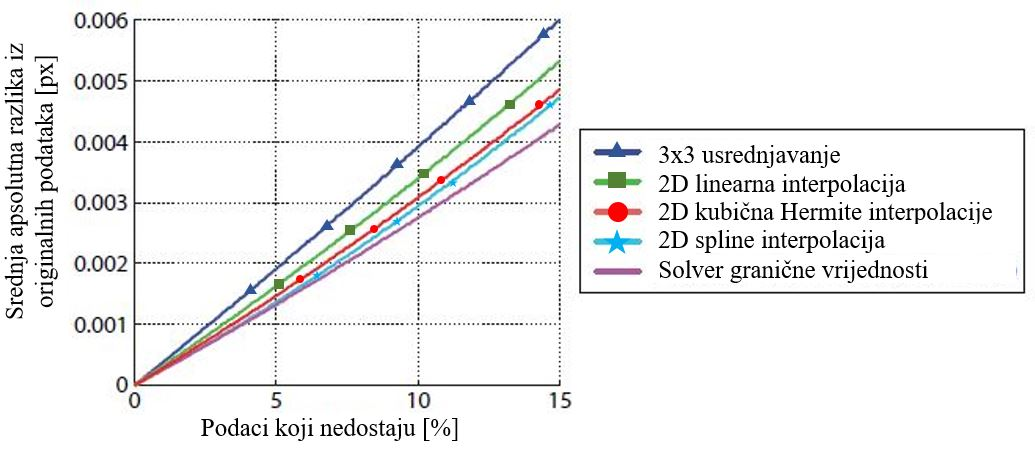
\includegraphics[width=14cm]{./2_DPIV/2_14PrefInterpolacije.jpg} 
	\caption{Performanse najčešće korištenih interpolacijskih shema. Solver granične vrijednosti ima najbolje rezultate za za PIV mjerenja gdje nedostaje mnogo podatka ($>10\%$) \cite{thielicke2014_phd}}
	\label{sl:2.14}
\end{figure}
\par
U novije vrijeme razvijen je napredniji algoritam zaglađivanja podataka koji se naziva "\textit{Smoothn}" \cite{garcia2010robust}, te je baziran na penalizirajućoj metodi najmanjih kvadrata. Na \textit{Slici \ref{sl:2.15}} prikazana je prosječna i maksimalna apsolutna razlika između točnih i izračunatih vrijednosti kod korištenja tri algoritma za zaglađivanje, te kod podataka koji nisu podvrgnuti niti jednom algoritmu za zaglađivanje. Sa slike je vidljivo kako korištenje algoritma daje podatke koji imaju mnogo manje šuma, te samim time povećavana je kvaliteta procjene brzine.
U PIVlab softver implementiran je "Smoothn" algoritam.
\begin{figure}[h]  
	\centering
	%\usepackage{graphicx}
	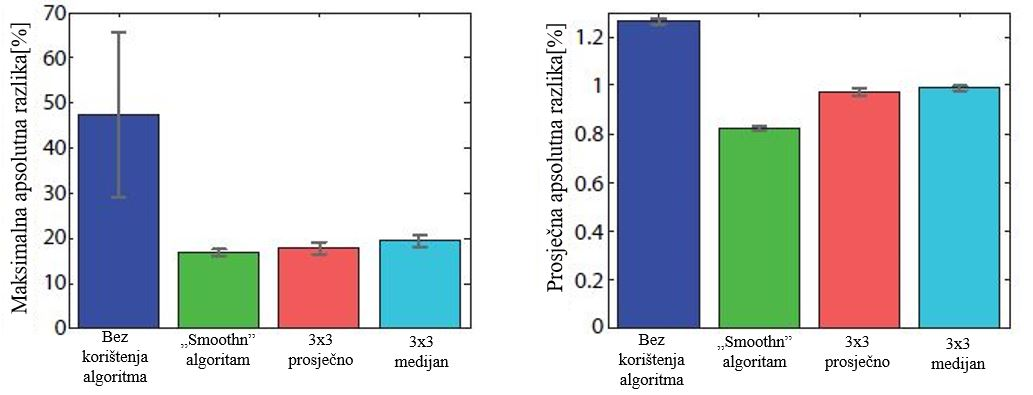
\includegraphics[width=16cm]{./2_DPIV/2_15AlgoritmiZaZagladivanje.jpg} 
	\caption{Validacija algoritama za zaglađivanje. Usporedba između maksimalnih i prosječnih izračunatih brzina i točnih podataka \cite{thielicke2014_phd}.}
	\label{sl:2.15}
\end{figure}
\FloatBarrier
\subsection{Korištenje vektorskih operatora}
Mnoga promatrana strujanja otkrivaju kompleksne uzorke koje je teško opisati samo sa mapom polja brzina, stoga ako ja moguće dobivene PIV podatke treba dalje obraditi i pojednostavniti. Nadalje, informacije o brzini često nisu glavni fizički interes strujanja, nego da bi strujanje bilo do kraja razriješeno potrebno je saznati informacije o polju tlakova i gustoća, jer to su preostali članovi Navier-Stokesove jednadžbe kojom se opisuje ponašanja fluida:
\begin{equation}
	\rho \dfrac{\mathrm{D}\boldsymbol{U}}{\mathrm{D}t}=-\nabla p+ \mu \nabla^{2}\boldsymbol{U}+\boldsymbol{f}
	\label{eqn:2.14}
\end{equation}
gdje $\boldsymbol{f}$ predstavlja doprinos masenih sila (npr. gravitacija). Načini na koji se dobivaju tlak i gustoća predmet je najnovijih PIV istraživanja i tehnologija (tomografski PIV, Shake-The-Box PIV,...). No ipak, 2D PIV i sam omogućava procjenu drugih fizički relevantnih veličina postupcima diferencijacije i integracije.
\par
Kod diferencijacije poseban interes ima polje vrtloga (rotacije) zbog toga što ova veličina, za razliku od polja brzina je neovisna o referentnom okviru. Posebno, ako je vremenski razriješeno, polje vrtloga može biti mnogo više korisno u proučavanju strujanja, pogotovo u strujanjima gdje ima mnogo vrtloga i turbulencija. Za nestlačivo strujanje ($\nabla \cdot \boldsymbol{U}=0$) Navier-Stokesova jednadžba može se zapisati pod uvjetima vrtloženja:
\begin{equation}
	\dfrac{\partial \boldsymbol{\omega}}{\partial t}+\boldsymbol{U}\cdot\nabla\boldsymbol{\omega}=\boldsymbol{\omega}\cdot\nabla\boldsymbol{U}+\nu\nabla^{2}\boldsymbol{\omega}
	\label{eqn:2.15}
\end{equation}
gdje se opisuje stopa promjene vrtloženja fluidnog elementa. U jednadžbi \ref{eqn:2.15} radi jednostavnosti izostavljen je član koji opisuje masene sile ($\boldsymbol{f}=0$), te se može primijetiti kako više nema člana koji opisuje tlak. No ipak usprkos prikazanim pojednostavljenjima posljednji član $\nabla^{2}\boldsymbol{\omega}$ i dalje je teško odrediti iz PIV podataka.
\subsection{Procjena diferencijalnih veličina}
Prije samog računanja diferencijalnih veličina iz polja podataka o brzinama treba odrediti koje se sve veličine uopće mogu izvući iz ravninskog polja brzina. Standardni 2D PIV naravno omogućuje samo dvo-komponentno polje brzina (zanemarena činjenica da 2D PIV daje 2D projekciju 3D vektora), dok je sa ostalim nadogradnjama PIV tehnologije (npr. stereoskopski PIV, tomografski PIV,...) moguće dobiti i polje brzina sa sve tri komponente. Za početak, kod 2D PIV mjerenja iz samo jednom snimane laserske ravnine (isključeno računanje gradijenata brzine u smjeru normalnom na ravninu) dan je izraz za tenzor promjene brzine (ili tenzor deformacija) $\mathrm{d}\boldsymbol{U}/\mathrm{d}\boldsymbol{X}$:
\begin{subequations}\label{eqn:2.16}
	\begin{equation}
		\dfrac{\mathrm{d}\boldsymbol{U}}{\mathrm{d}\boldsymbol{X}} = 
		\begin{bmatrix}
			\dfrac{\partial U}{\partial X}       &   \dfrac{\partial V}{\partial X}       &   \dfrac{\partial W}{\partial X}       \\
			\dfrac{\partial U}{\partial Y}       &   \dfrac{\partial V}{\partial Y}       &   \dfrac{\partial W}{\partial Y}       \\   
			\dfrac{\partial U}{\partial Z}       &   \dfrac{\partial V}{\partial Z}       &   \dfrac{\partial W}{\partial Z}       \\
		\end{bmatrix}
	\tag{\ref{eqn:2.16}}
	\end{equation}
	Tenzor deformacija može se raščlaniti na svoj simetrični i antisimetrični dio:
	\begin{align}\label{eqn:2.16a}
		\dfrac{\mathrm{d}\boldsymbol{U}}{\mathrm{d}\boldsymbol{X}} = 
		&\underbrace{\begin{bmatrix}
				\dfrac{\partial U}{\partial X}       &   \dfrac{1}{2}\left(\dfrac{\partial V}{\partial X}+\dfrac{\partial U}{\partial Y}\right)       &   \dfrac{1}{2}\left(\dfrac{\partial W}{\partial X}+\dfrac{\partial U}{\partial Z}\right)       \\
				\dfrac{1}{2}\left(\dfrac{\partial U}{\partial Y}+\dfrac{\partial V}{\partial X}\right)       &   \dfrac{\partial V}{\partial Y}       &   \dfrac{1}{2}\left(\dfrac{\partial W}{\partial Y}+\dfrac{\partial V}{\partial Z}\right)       \\   
				\dfrac{1}{2}\left(\dfrac{\partial U}{\partial Z}+\dfrac{\partial W}{\partial X}\right)       &   \dfrac{1}{2}\left(\dfrac{\partial V}{\partial Z}+\dfrac{\partial W}{\partial Y}\right)       &   \dfrac{\partial W}{\partial Z}       \\
		\end{bmatrix}}_{\text{simetr.}} \notag \\
		&+ \underbrace{\begin{bmatrix}
				0       &   \dfrac{1}{2}\left(\dfrac{\partial V}{\partial X}-\dfrac{\partial U}{\partial Y}\right)       &   \dfrac{1}{2}\left(\dfrac{\partial W}{\partial X}-\dfrac{\partial U}{\partial Z}\right)       \\
				\dfrac{1}{2}\left(\dfrac{\partial U}{\partial Y}-\dfrac{\partial V}{\partial X}\right)       &   0       &   \dfrac{1}{2}\left(\dfrac{\partial W}{\partial Y}-\dfrac{\partial V}{\partial Z}\right)       \\   
				\dfrac{1}{2}\left(\dfrac{\partial U}{\partial Z}-\dfrac{\partial W}{\partial X}\right)       &   \dfrac{1}{2}\left(\dfrac{\partial V}{\partial Z}-\dfrac{\partial W}{\partial Y}\right)       &   0       \\
		\end{bmatrix}}_{\text{antisimetr.}}
	\end{align}
\end{subequations}
Ako članove u jednadžbi \ref{eqn:2.16a} zamijenimo sa komponentama deformacije i rotacije jednadžba ima oblik:
\begin{equation}
	\dfrac{\mathrm{d}\boldsymbol{U}}{\mathrm{d}\boldsymbol{X}} = 
	\underbrace{\begin{bmatrix}
			\epsilon_{XX}       &   \dfrac{1}{2}\epsilon_{XY}       &   \dfrac{1}{2}\epsilon_{XZ}       \\
			\dfrac{1}{2}\epsilon_{YX}       &   \epsilon_{YY}       &   \dfrac{1}{2}\epsilon_{YZ}       \\   
			\dfrac{1}{2}\epsilon_{ZX}       &   \dfrac{1}{2}\epsilon_{ZY}       &   \epsilon_{ZZ}       \\
	\end{bmatrix}}_{\text{matrica brzina deformacije}} + 
	\underbrace{\begin{bmatrix}
			0       &   \dfrac{1}{2}\omega_{Z}       &   -\dfrac{1}{2}\omega_{X}       \\
			-\dfrac{1}{2}\omega_{Z}       &   0       &   \dfrac{1}{2}\omega_{Y}       \\   
			-\dfrac{1}{2}\omega_{X}       &   \dfrac{1}{2}\omega_{Y}       &   0       \\
	\end{bmatrix}}_{\text{matrica rotacije}}
	\label{eqn:2.17}
\end{equation}
gdje dijagonalni članovi matrice brzine deformacije predstavljaju deformaciju zbog produljenja, a van-dijagonalni članovi predstavljaju deformaciju zbog smicanja, dok svi članovi matrice rotacije predstavljaju komponente rotacije.
\par
Kako konvencionalni 2D PIV omogućava samo $U$ i $V$ komponente brzine, te samim time svi podaci mogu se diferencirati samo u $X$ i $Y$ smjeru, samo se nekoliko članova tenzora deformacije $\mathrm{d}\boldsymbol{U}/\mathrm{d}\boldsymbol{X}$ može procijeniti sa PIV podacima. Najčešći parametri korišteni za vizualizaciju gradijenata u strujanju prikazani su u \textit{Tablici \ref{tab:2.2}}. Ovi parametri su izračunati uz pomoć lokalne stope promjene brzine (derivacije brzine).
\begin{table}[h]
	\centering
	\caption{Gradijentni parametri koji se mogu izvesti iz informacija o brzinama strujanja dobivenih putem 2D-PIV, te dodatno pomoći pri interpretaciji promatranog strujanja \cite{stamhuis2006basics}}
	\resizebox{\textwidth}{!}{%
	\begin{tabular}{cll}
		\hline
		\rowcolor[HTML]{9B9B9B} 
		\textbf{Parametar}                                                              & \textbf{Predstavlja:}                                                                                                                               & \textbf{Jednadžba}                                                                          \\ \hline
		\begin{tabular}[c]{@{}c@{}}Vrtložnost\\ (\textit{eng.vorticity})\end{tabular}            & \begin{tabular}[c]{@{}l@{}}Rotaciju fluida\\ ("komponenta rotacije normalna na lasersku ravninu")\end{tabular}                                      & $\omega_{Z}=\dfrac{\partial V}{\partial X}-\dfrac{\partial U}{\partial Y}$                  \\ \hline
		\begin{tabular}[c]{@{}c@{}}Stopa smicanja\\ (\textit{eng. shear rate})\end{tabular}      & \begin{tabular}[c]{@{}l@{}}Jačinu gradijenta brzine okomito na lokalnu brzinu\\ ("unutar-ravninsko klizanje susjednih slojeva fluida")\end{tabular} & $\epsilon_{XY}=\dfrac{\partial U}{\partial Y}+\dfrac{\partial V}{\partial X}$               \\ \hline
		\begin{tabular}[c]{@{}c@{}}Stopa istezanja\\ (\textit{eng. strain rate})\end{tabular}    & \begin{tabular}[c]{@{}l@{}}Jačina gradijenta brzine u smjeru lokalne brzine\\ ("unutar-ravninsko ubrzanje unutar jednog sloja fluida")\end{tabular} & $\epsilon_{XX}-\epsilon_{YY}=\dfrac{\partial U}{\partial X}-\dfrac{\partial V}{\partial Y}$ \\ \hline
		Divergenca                                                                      & \begin{tabular}[c]{@{}l@{}}Jačina izvan-ravninske stope strujanja\\ ("struja koja napušta i ulazi u lasersku ravninu")\end{tabular}                 & $\eta=\epsilon_{XX}+\epsilon_{YY}=\dfrac{\partial U}{\partial X}+\dfrac{\partial V}{\partial Y}$ \\ \hline
		\begin{tabular}[c]{@{}c@{}}Lokator vrtloga\\ (\textit{eng. vortex locator})\end{tabular} & \begin{tabular}[c]{@{}l@{}}Pronalazi centar vrtloga\\ (preko diskriminante za  kompleksne svojstvene vrijednosti)\end{tabular}                      &                                                                                             \\ \hline
	\end{tabular}}
\label{tab:2.2}
\end{table}
\par
Samo komponenta rotacije normalna na lasersku ravninu $\omega_{Z}$ može biti određena, zajedno sa unutar-ravninskim smicanjem $\epsilon_{XY}$ i divergencom $\eta$. Zanimljivo je napomenuti kako postojanje treće komponente brzine $W$, koja se dobije sa naprimjer stereoskopskim PIV mjerenjem ne daje nikakve dodatne komponente deformacije ili rotacije. Ako se pretpostavi nestlačivo strujanje ($\nabla \cdot \boldsymbol{U}=0$), suma unutar-ravninskih deformacija u jednadžbi za $\eta$ iz \textit{Tablice \ref{tab:2.2}} može biti iskorištena za procjenu izvan-ravninskog strujanja $\epsilon_{ZZ}$:
\begin{equation*}
	\epsilon_{ZZ}=\dfrac{\partial W}{\partial Z}=-\dfrac{\partial U}{\partial X}-\dfrac{\partial V}{\partial Y}=-\eta
\end{equation*}
Međutim potrebno je napomenuti kako veličina $\eta$ samo upućuje na prisutnost izvan-ravninskog strujanja, ali ne daje nikakve informacije o van-ravninskoj brzini $W$.
\FloatBarrier
\subsection{Procjena integralnih veličina}
\begin{description}[style=unboxed,leftmargin=0cm]
	\item[Linijski integral - Cirukulacija] Po definiciji, vrtloženje integrirano nad područjem $A$ jednako je cirkulaciji $\Gamma$. Stokesov teorem daje vezu između vrtloženja i cirkulacije, te uz pomoć njega operacija integriranja se reducira na linijski integral skalarnog produkta između lokalnog vektora brzine $\boldsymbol{U}$ i djelića elementa putanje vektora $d\boldsymbol{X}$, gdje je putanja integracije određena granicom $C$ zatvorenog područja $A$:
	\begin{align}
		\begin{split} \label{eqn:2.18}
			\Gamma&=\int_{A}\omega \, dA
		\end{split} \\
		\begin{split} \label{eqn:2.19}
			&=\oint_{C}\boldsymbol{U}\cdot d\boldsymbol{X}
		\end{split}
	\end{align}
	Za dvo-komponentne PIV podatke o brzinama u $XY$ ravnini sa $\boldsymbol{U}\, =\, (U,V)$, gornja jednadžba se svede na:
	\begin{align}
		\begin{split} \label{eqn:2.20}
			\Gamma&=\int \int_{A(X,Y)}\omega_{Z}\, dX \, dY
		\end{split} \\
		\begin{split} \label{eqn:2.21}
			&=\oint_{C(X,Y)}\boldsymbol{U}(\boldsymbol{X}, \boldsymbol{Y})\cdot d\boldsymbol{X}
		\end{split} \\
		\begin{split} \label{eqn:2.22}
			&=\oint_{C(X,Y)}U \, dX+V \, dY
		\end{split}
	\end{align}
	Sa zadanim putem integracije, moguće je izravno rješavanje jednadžbe \ref{eqn:2.22} koristeći jednu od integracijskih shema (npr. trapezna aproksimacija, Simpsonovo pravilo , ...). Kod određivanja cirkulacije jasno definirane, skoro kružne vrtložne strukture, obično je dovoljno zadati kružni put integracije centriran na maksimumu vrtložnosti. Iscrtavanjem cirkulacije s obzirom na polumjer puta integracije, može se primijeniti asimptotska konvergencija prema vrijednosti cirkulacije strukture. Ova konvergencija poklapa se sa opadanjem (raspadom) vrtložnosti dalje od jezgre vrtloga. 
	\par
	Zadavanje razumnog puta integracije za složenije vrtložne strukture nije jednostavno kao inače. Za vrtložne strukture, idealno bi bilo kada bi put integracije bio definiran dijeljenjem linije toka na kojoj se vrtložna struktura odvaja jedna od druge. No ipak računanje funkcije toka iz nestacionarnih podataka o brzini je jako složeno i često se ne dobije jedinstveno rješenje.
	\item[Linijski integral - maseni protok] Za određene primjene, zanimljivo je izračunati intenzitet masenog ili volumenskog protoka preko kontrolne površine KA:
	\begin{equation}
		\boldsymbol{\dot{M}}=\frac{dm}{dt}=\int \int_{KA}\rho(\boldsymbol{U}\cdot \boldsymbol{\hat{n}})dA
		\label{eqn:2.23}
	\end{equation}
	Za 2D podatke u XY ravnini, površina se reducira na put integracije slično kao i kod jednadžbe \ref{eqn:2.22}:
	\begin{equation}
		\boldsymbol{\dot{M}}_{XY}=\frac{dm_{XY}}{dt}=\oint_{C}\rho(U \, dY-V \, dX)
		\label{eqn:2.24}
	\end{equation}
	Jedinica kojom se izražava $\boldsymbol{\dot{M}}_{XY}$ je maseni protok (kg) po jedinici dubine, te ako je $\rho \equiv 1$, tada jednadžba \ref{eqn:2.24} predstavlja intenzitet volumenskog protoka po jedinici dubine. 
	\item[Tlak i sile iz PIV podataka] Osnovni princip izvlačenja tlaka i sila iz PIV podataka je taj da Navier-Stokesova jednadžba povezuje lokalni gradijent tlaka sa ubrzanjem fluida i članom viskoznog naprezanja. Za nestlačivo strujanje (konstantan $\rho$ i viskoznost $\mu$) moguće je dobivanje gradijenta tlaka $\nabla p$ direktno iz izmjerenog polja brzina $\boldsymbol{U}$:
	\begin{equation}
		\nabla p = -\rho \frac{D\boldsymbol{U}}{Dt}+\mu \nabla^{2}\boldsymbol{U}=-\rho \left(\frac{\partial \boldsymbol{U}}{\partial t}+(\boldsymbol{U}\cdot\nabla)\boldsymbol{U}\right)+\mu \nabla^{2}\boldsymbol{U}
		\label{eqn:2.25}
	\end{equation}
	Posljednji viskozni član iz jednadžbe \ref{eqn:2.25} moguće je izračunati kako bi se dobili potpuni rezultati, međutim potvrđeno je kako doprinos viskoznog člana računanju tlaka u većini slučajeva zanemariv, te se u općenito koristi sljedeći oblik gornje jednadžbe:
	\begin{equation}
		\nabla p = -\rho \left(\frac{\partial \boldsymbol{U}}{\partial t}+(\boldsymbol{U}\cdot\nabla)\boldsymbol{U}\right)
		\label{eqn:2.26}
	\end{equation}
	Nadalje, određivanjem cirkulacije vrtloga koja je ranije opisana, moguća je primjena Kutta-Joukowski teorema kako bi se izvele sile koje djeluju na tijelo unutar fluida (primjer u literaturi \cite{henningsson2011time}). Opisane značajke su implementirane u PIVlab softver, te značajno pojednostavljuju određivanje cirkulacije i primjene Kutta-Joukowski teorema.
\end{description}
\chapter{MATEMATIČKA POZADINA STATISTIČKE PIV EVALUACIJE}
\label{chap:Poglavlje_3}
U ovom poglavlju prikazan je pojednostavljeni opis matematičkog modela snimanja, te statističke evaluacije PIV snimki. Analizirana je kros-korelacija na dva kadra (snimke), svaka snimka je izložena jednoj ekspoziciji. Matematičku teoriju evaluacije više-ekspozicioniranih snimki moguće je pronaći u literaturi \cite{raffel2018_book}.
\section{Položaj čestica na snimkama}
PIV snimke su tijekom evaluacije podijeljene na prozore ispitivanja. Važno je napomenuti kako su PIV snimke 2-dimenzionalne, dok osvijetljena laserska ploha ima određenu debljinu (treću dimenziju). Geometrijska projekcija PIV slika na lasersku osvijetljenu ravninu prikazana je na \textit{Slici \ref{sl:3.1}}.
\begin{figure}[h]  
	\centering
	%\usepackage{graphicx}
	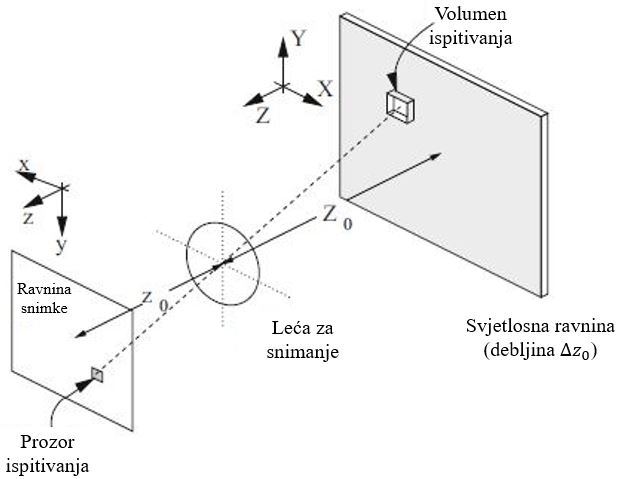
\includegraphics[width=11cm]{./3_MatPozadina/3_1ShemaPIVsnimki.jpg} 
	\caption{Shematski prikaz geometrije snimanja\cite{raffel2018_book}}
	\label{sl:3.1}
\end{figure}
\par
Neka se razmatra snimka pri jednoj ekspoziciji. Na snimci se nalaze slučajno distribuirane slike čestica, koje odgovaraju $N$ broju čestica markera ubačenih u strujanje:
\begin{equation}
	\boldsymbol{\Gamma} = \left[ \begin{array}{c}
						\boldsymbol{X_{1}} \\
						\boldsymbol{X_{2}} \\
						\vdots \\
						\boldsymbol{X_{N}}
					\end{array} \right]
\label{eqn:3.1}
\end{equation}
gdje je $\boldsymbol{X_{i}}=\left(X_{i}, Y_{i}, Z_{i}\right)$ vektor pozicije čestice $i$ u trenutku $t$. $\boldsymbol{\Gamma}$ opisuje stanje cjeline u trenutku $t$. Jednadžba \ref{eqn:3.1} označava poziciju čestica u 3D prostoru (volumena ispitivanja). Malim slovim će se označavati koordinate čestica na ravnini snimke (\textit{Slika \ref{sl:3.1}}) tako da $x$ označava poziciju čestice na snimci:
\begin{equation}
	\boldsymbol{x} = \left[ \begin{array}{c}
		x\\
		y
	\end{array}\right]
\label{eqn:3.2}
\end{equation}
Radi jednostavnosti pretpostavit će se kako su pozicije čestica u volumenu ispitivanja i njene pozicije u ravnini snimke povezane konstantnim faktorom povećanja $M$ tako da vrijedi:
\begin{equation}
	\boldsymbol{X_{i}}=\dfrac{\boldsymbol{x_{i}}}{M} \quad\text{i}\quad \boldsymbol{Y_{i}}=\dfrac{\boldsymbol{y_{i}}}{M}
\label{eqn:3.3}
\end{equation}
\FloatBarrier
\section{Polje intenziteta snimke}
U ovom dijelu prikazan je intenzitet distribucije vrijednosti u ravnini snimke. Pretpostavlja se kako snimka najbolje može biti opisana konvolucijom geometrijske slike i impulsnog odziva sustava snimanja, tkv. funkcijom širenja točke PSF (\textit{eng. point spread function}) \cite{raffel2018_book}. PSF se u mnogim kontekstima može smatrati proširenom mrljom jedne čestice (\textit{Slika \ref{sl:3.2}}), to jest mjerom koliko će se točka (čestica) proširiti zbog loše kvalitet sustava snimanja \cite{wiki:Point_spread_function}. Za infinitezimalno malenu česticu i bez aberacije fokusiranu leću, amplituda PSF-a matematički je opisana Airy-ovom funkcijom (Bessel-ova funkcija prvog reda).
\begin{figure}[h]  
	\centering
	%\usepackage{graphicx}
	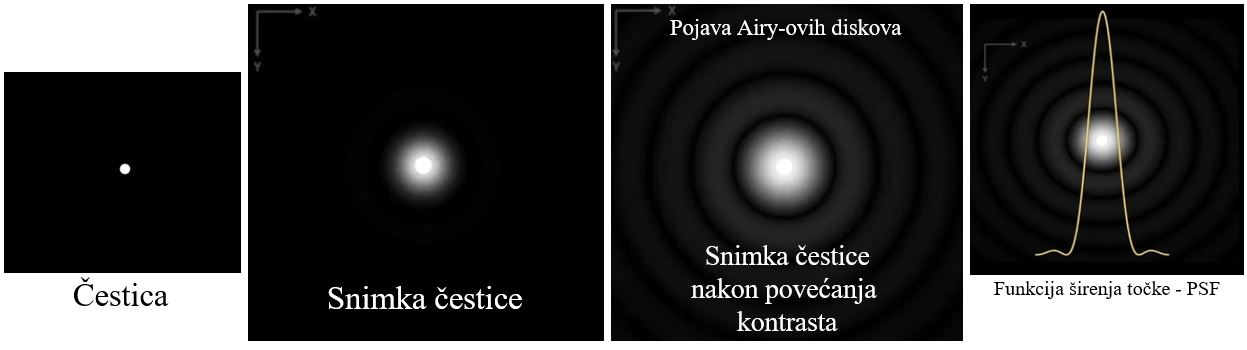
\includegraphics[width=15cm]{./3_MatPozadina/3_2PSF.jpg} 
	\caption{PSF i pojava Airy-ovih diskova \cite{youtube_PSF}}
	\label{sl:3.2}
\end{figure}
\par
U ovoj analizi pretpostaviti će se da funkcija širenja točke PSF leće za snimanje $\tau (\boldsymbol{x})$ ima sličan oblik Gauss-ovoj funkciji, što je uobičajena praksa i dobra aproksimacija za PSF leće za snimanje u stvarnom slučaju:
\begin{equation}
	\tau (\boldsymbol{x}) = K \, \exp \left(-\dfrac{8|\boldsymbol{x}|^2}{d_{\tau}^{2}}\right)
	\label{eqn:3.4}
\end{equation}
gdje je:
\begin{equation*}
	K = \dfrac{8\tau_{0}}{\pi d_{\tau}^{2}}
\end{equation*}
$d_{\tau}$ predstavlja razliku između stvarnog i idealnog promjera čestice na snimci. Konvolucijski produkt $\tau (\boldsymbol{x})$ sa geometrijskom slikom čestice markera na poziciji $\boldsymbol{x_{i}}$ opisuje položaj jedne čestice na poziciji $\boldsymbol{X_{i}}$. Nadalje, analiza će se ograničiti na infinitezimalno male geometrijske slike čestica, što je inače slučaj kod snimanja malenih čestica na malim uvećanjima. Stoga se koristi Dirac delta-funkcija pomaknuta na poziciju $\boldsymbol{x_{i}}$ kako bi se opisao geometrijski dio slike čestice. Na ovaj način polje intenziteta snimke (\textit{Slika \ref{sl:3.3}}) prilikom jedne ekspozicije može biti dano izrazom:
\begin{equation}
	I = I (\boldsymbol{x}, \boldsymbol{\Gamma}) = \tau (\boldsymbol{x}) \ast \sum_{i=1}^{N}V_{0}(\boldsymbol{X_{i}}) \, \delta (\boldsymbol{x}-\boldsymbol{x_{i}})
	\label{eqn:3.5}
\end{equation}
gdje je $V_{0} (\boldsymbol{X_{i}})$ transfer funkcija koja je dana energijom svijetla slike jedne čestice $i$ unutar volumena ispitivanja $V_{I}$  i njenom konverzijom u električni signal. $\tau (\boldsymbol{x})$ se smatra identičnim za svaku poziciju čestice. Vidljivost čestice ovisi o mnogo parametara, a jedni od važnijih su: svojstvo čestice da raspršuje svjetlost, jačina svjetlosti na mjestu gdje se nalazi čestica, osjetljivost optike za snimanje, kvaliteta senzora na kameri. Ovdje će se pretpostaviti kako čestice na svakoj poziciji imaju ista svojstva raspršivanja, te ostala tehnika za snimanje također ima ista svojstva. Potrebno je napomenuti kako u slučaju različitih svojstava, moguće je množenje različitih prozora ispitivanja za različitim kernelima koji će ta svojstva "ispeglati".
\begin{figure}[h]  
	\centering
	%\usepackage{graphicx}
	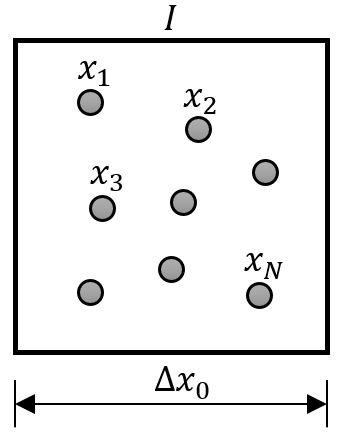
\includegraphics[width=3cm]{./3_MatPozadina/3_3primjerPoljaCestica.jpg} 
	\caption{Primjer polja $I$ prilikom samo jedne ekspozicije}
	\label{sl:3.3}
\end{figure}
\par
Nadalje, neka $Z$ predstavlja smjer gledanja, intenzitet svjetla unutar područja ispitivanja je tako jedino u funkciji $Z$ i na kraju analizirani intenzitet snimke jedino ovisi o $X$ i $Y$. Stoga, $V_{0} (\boldsymbol{X})$ opisuje oblik, produženje i lokaciju stvarnog volumena ispitivanja.
\begin{equation}
	V_{0}(\boldsymbol{X}) = W_{0}(X, Y)\, I_{0}(Z)
	\label{eqn:3.6}
\end{equation}
gdje je $I_{0}(z)$ profil intenziteta laserske zrake u $Z$ smjeru, a $W_{0}(X, Y)$ funkcija prozora ispitivanja geometrijski projicirana na svjetlosnu ravninu. Treba napomenuti kako ovo matematički nije točno zbog toga što nije uzeta u obzir konvolucija sa funkcijom širenja točke PSF. Samim time može se zaključiti kako za prozore ispitivanja u obliku pravokutnika u prikazanom matematičkom opisu zanemaren je efekt djelomično obrezanih (\textit{eng. cropped}) snimki na rubovima područja ispitivanja. Međutim, ovaj jednostavni model prozora ispitivanja će se koristiti u strujanju zbog toga što pojednostavljuje opis PIV evaluacije. Izraz
\begin{equation}
	I_{o}(Z) = I_{Z}\, \exp\left(-8\dfrac{(Z-Z_{0})^{2}}{\Delta Z_{0}^{2}}\right)
	\label{eqn:3.7}
\end{equation}
će se korisiti kako bi se opisao Gauss-ov profil intenziteta u $Z$ smjeru laserske svjetlosne ravnine. $\Delta Z_{0}$ predstavlja debljinu svjetlosne ravnine, a $I_{Z}$ je maksimalna vrijednost intenziteta svjetlosne ravnine. Funkcija $W_{0}(X, Y)$ također je opisana Gauss-ovom funkcijom u kojoj uzimamo u obzir maksimalni težinski faktor $W_{XY}$ na poziciji $X_{0}$, $Y_{0}$:
\begin{equation}
	W_{0}(X, Y)=W_{XY}\, \exp \left(-8\dfrac{(X-X_{0})^{2}}{\Delta X_{0}^{2}}-8\dfrac{(Y-Y_{0})^{2}}{\Delta Y_{0}^{2}}\right)
	\label{eqn:3.8}
\end{equation}
Osim Gauss-ovom funkcijom, intenzitet distribucije laserske ravnine može (jednostavnije) biti opisan i sa top-hat funkcijom. U tom slučaju $I_{0}(Z)$ i $W_{0}(X, Y)$ imaju oblik:
\begin{equation}
	I_{0}(Z))=\begin{cases}
		I_{Z} &\text{ako je}\quad |Z-Z_{0}|\leq \dfrac{\Delta Z_{0}}{2}\\
		0 &\text{inače}
	\end{cases}
	\label{eqn:3.9}
\end{equation}
\begin{equation}
	W_{0}(X, Y))=\begin{cases}
		W_{XY} &\text{ako je}\quad |X-X_{0}|\leq \dfrac{\Delta X_{0}}{2}\quad \text{i}\quad |Y-Y_{0}|\leq \dfrac{\Delta Y_{0}}{2}\\
		0 &\text{inače}
	\end{cases}
	\label{eqn:3.10}
\end{equation}
Faktor $I_{0}(Z_{i})$ predstavlja primljenu količinu svjetla od čestice $i$ unutar strujanja lociranu na udaljenosti $|Z_{i}-Z{0}|$ od središnje ravnine laserske plahte. $\Delta Z_{0}$ je debljina laserske ravnine (ekstenzija volumena ispitivanja u $Z$ smjeru), dok su $\Delta X_{0}=\Delta x_{0}/M$ i $\Delta Y_{0}=\Delta y_{0}/M$ ekstenzije volumena ispitivanja u $X$ i $Y$ smjeru. Ako je funkcija širenje točke (PSF) $\tau (\boldsymbol{x}-\boldsymbol{x_{i}})=\tau \ast \delta (\boldsymbol{x}-\boldsymbol{x_{i}})$ i ako se uzme pretpostavka da promatrane snimke čestica se ne preklapaju jednažba \ref{eqn:3.5} alternativno se može zapisati:
\begin{equation}
	I(\boldsymbol{x}, \boldsymbol{\Gamma})=\sum_{i=1}^{N}V_{0}(\boldsymbol{X_{i}})\, \tau (\boldsymbol{x}-\boldsymbol{x_{i}})
	\label{eqn:3.11}
\end{equation}
Jednadžba \ref{eqn:3.11} predstavlja polje intenziteta snimke, te će ovaj izraz biti korišten u opisu korelacije dane primjerom sa tri proizvoljno pozicionirane čestice.
\FloatBarrier
\section{Srednja vrijednost, auto-korelacija i varijanca jednom ekspozicionirane snimke}
U ovom dijelu prikazati će se pojmovi auto-korelacije i auto-kovarijance jednom ekspozicionirane snimke. Također, biti će određeni srednja vrijednost i varijanca, koje su bitne vrijednosti polja intenziteta snimke jer se uz pomoć njih vrši normalizacija kros-korelacije. Prostorni prosjek je definiran izrazom \cite{raffel2018_book}:
\begin{equation}
	\langle I(\boldsymbol{x}, \boldsymbol{\Gamma})\rangle =\dfrac{1}{a_{I}}\int_{a_{I}}I(\boldsymbol{x}, \boldsymbol{\Gamma})dx
	\label{eqn:3.12}
\end{equation}
gdje $a_{I}$ predstavlja područje ispitivanje. Uvrštavanjem jednadžbe \ref{eqn:3.11} u \ref{eqn:3.12} dobije se:
\begin{equation}
	\langle I(\boldsymbol{x}, \boldsymbol{\Gamma})\rangle =\dfrac{1}{a_{I}}\int_{a_{I}}\sum_{i=1}^{N}V_{0}(\boldsymbol{X_{i}})\, \tau (\boldsymbol{x}-\boldsymbol{x_{i}})dx
	\label{eqn:3.13}
\end{equation}
Srednja vrijednost polja intenziteta može biti aproksimirana sa:
\begin{equation}
	\mu_{I}=\langle I(\boldsymbol{x}, \boldsymbol{\Gamma})\rangle =\dfrac{1}{a_{I}}\sum_{i=1}^{N}V_{0}(\boldsymbol{X_{i}}\int_{a_{I}}\tau (\boldsymbol{x}-\boldsymbol{x_{i}}))dx
	\label{eqn:3.14}
\end{equation}
Sada je moguće izvesti auto-korelaciju jednom ekspozicioniranog polja intenziteta na sličan način:
\begin{equation}
	\begin{split}
		R_{I}(\boldsymbol{s}, \boldsymbol{\Gamma}) &= \langle I(\boldsymbol{x}, \boldsymbol{\Gamma})\, I(\boldsymbol{x}+\boldsymbol{s}, \boldsymbol{\Gamma})\rangle\\
		 &= \dfrac{1}{a_{I}}\int_{a_{I}}\sum_{i=1}^{N}V_{0}(\boldsymbol{X_{i}})\, \tau (\boldsymbol{x}-\boldsymbol{x_{i}})\sum_{j=1}^{N}V_{0}(\boldsymbol{X_{j}})\, \tau (\boldsymbol{x}-\boldsymbol{x_{j}}+\boldsymbol{s})dx
		 \label{eqn:3.15}
	\end{split}
\end{equation}
gdje $s$ predstavlja vektor separacije u korelacijskoj ravnini. Razlikovanjem $i\neq j$ članova koji predstavljaju korelaciju različitih snimki čestica, te samim time nasumično distribuirani šum u korelacijskoj ravnini od $i=j$ koji predstavljaju korelaciju svake čestice same sa sobom, izraz \ref{eqn:3.15} može se konačno zapisati kao:
\begin{equation}
	\begin{split}
		R_{I}(\boldsymbol{s}, \boldsymbol{\Gamma}) = &\dfrac{1}{a_{I}}\sum_{i\neq j}^{N}V_{0}(\boldsymbol{X_{i}})\, V_{0}(\boldsymbol{X_{j}})\int_{a_{I}}\tau (\boldsymbol{x}-\boldsymbol{x_{i}})\, \tau (\boldsymbol{x}-\boldsymbol{x_{j}}-\boldsymbol{s})dx\\
		 &+ \dfrac{1}{a_{I}}\sum_{i=j}^{N}V_{0}^{2}(\boldsymbol{X_{i}})\int_{a_{I}}\tau (\boldsymbol{x}-\boldsymbol{x_{i}})\, \tau (\boldsymbol{x}-\boldsymbol{x_{j}}-\boldsymbol{s})dx
	\end{split}
	\label{eqn:3.16}
\end{equation}
Jednadžbu \ref{eqn:3.16} moguće je raščlaniti i zapisati u obliku \cite{raffel2018_book}:
\begin{equation}
	R_{I}(\boldsymbol{s},\boldsymbol{\Gamma})=R_{C}(\boldsymbol{s},\boldsymbol{\Gamma})+R_{F}(\boldsymbol{s},\boldsymbol{\Gamma})+R_{P}(\boldsymbol{s},\boldsymbol{\Gamma})
	\label{eqn:3.17}
\end{equation}
gdje je: $R_{C}(\boldsymbol{s},\boldsymbol{\Gamma})$ kovolucija srednjih intenziteta $I$ (srednja pozadinska korelacija), $R_{F}(\boldsymbol{s},\boldsymbol{\Gamma})$ je fluktuirajuća komponenta šuma, te oba člana su rezultat $i\neq j$ članova. Dok, zadnji preostali član $R_{P}(\boldsymbol{s},\boldsymbol{\Gamma})$ predstavlja samo-korelacijski vrh na poziciji $(0, 0)$ u korelacijskoj ravnini i rezultat je $i=j$ članova (korelacija svih slika čestica samih sa sobom). Auto-korelacija podataka čestica sa snimke na \textit{Slici \ref{sl:3.3}} prikazana je na \textit{Slici \ref{sl:3.4}}, te jasno prikazan centralni korelacijski vrh $R_{P}$ i šum oko njega.
\begin{figure}[h]  
	\centering
	%\usepackage{graphicx}
	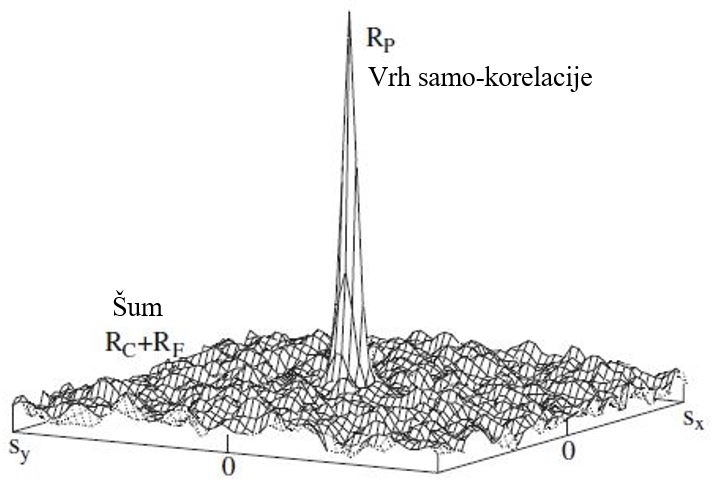
\includegraphics[width=9cm]{./3_MatPozadina/3_4AutoKorelacija.jpg} 
	\caption{Kompozicija vrhova u auto-korelacijskoj funkciji \cite{raffel2018_book}}
	\label{sl:3.4}
\end{figure}
\par
Ako auto-korelaciju sa \textit{Slike \ref{sl:3.4}} aproksimiramo Gauss-ovom funkcijom (jednadžba \ref{eqn:3.4}) koja ima širinu $\sqrt{2}d_{\tau}$ čime se zanemaruje šum, $R_{P}(\boldsymbol{s},\boldsymbol{\Gamma})$ se može zapisati kao:
\begin{equation}
	R_{P}(\boldsymbol{s},\boldsymbol{\Gamma}) = \sum_{i=1}^{N}V_{0}^{2}(\boldsymbol{X_{i}})\, \exp \left(\dfrac{-8|\boldsymbol{s}|^{2}}{d_{\tau}^{2}}\right)\dfrac{1}{a_{I}}\int_{a_{I}}\tau^{2}\left(\boldsymbol{x}-\boldsymbol{x_{i}}+\dfrac{\boldsymbol{s}}{2}\right)dx
	\label{eqn:3.18}
\end{equation}
U ovom radu korelacija snimke čestica $R_{\tau}(\boldsymbol{s})$ biti će prikazana izrazom:
\begin{equation}
	R_{\tau}(\boldsymbol{s})=\exp \left(\dfrac{-8|\boldsymbol{s}|^{2}}{d_{\tau}^{2}}\right)\dfrac{1}{a_{I}}\int_{a_{I}}\tau^{2}\left(\boldsymbol{x}-\boldsymbol{x_{i}}+\dfrac{\boldsymbol{s}}{2}\right)dx
	\label{eqn:3.19}
\end{equation}
pa samim time jednadžbu \ref{eqn:3.18} uvrštavanjem izraza \ref{eqn:3.19} može kraće zapisati kao:
\begin{equation}
	R_{P}(\boldsymbol{s},\boldsymbol{\Gamma})=R_{\tau}(\boldsymbol{s})\sum_{i=1}^{N}V_{0}^{2}(\boldsymbol{X_{i}})
	\label{eqn:3.20}
\end{equation}
Za polje intenziteta sa srednjom vrijednosti koja je jednaka nuli, auto-korelacija je jednaka auto-kovarijanci. Za ne-nula srednje vrijednosti polje intenziteta auto-kovarijance $C_{i}(s)$ može se dobiti izrazom \cite{raffel2018_book}:
\begin{equation}
	C_{I}(\boldsymbol{s})=R_{I}(\boldsymbol{s})-\mu_{I}^{2}
	\label{eqn:3.21}
\end{equation}
Procjena varijance tako ima oblik:
\begin{equation}
	\sigma_{I}^{2}=C_{I}(\boldsymbol{0}, \boldsymbol{\Gamma})=R_{I}(\boldsymbol{0}, \boldsymbol{\Gamma})-\mu_{I}^{2}=R_{P}(\boldsymbol{0}, \boldsymbol{\Gamma})-\mu_{I}^{2}
	\label{eqn:3.22}
\end{equation}
\FloatBarrier
\section{Kros-korelacija dvije uzastopne jednom ekspozicionirane snimke}
PIV snimke su obično evaluirane na način da se lokalno kros-koreliraju dvije uzastopne jednom ekspozicionirane snimke, te će u ovom potpoglavlju biti prikazan matematički opis spomenute kros-korelacije. Moguća je evaluacija i snimki koje su dva ili više puta ekspozicionirane (više u literaturi \cite{raffel2018_book}).\\
Za početak, potrebno je pretpostaviti vektor konstantnih pomaka $\boldsymbol{D}$ svih čestica unutar volumena ispitivanja, tako da se položaj čestica na snimici prilikom druge ekspozicije u trenutku $t' = t + \Delta t$ može zapisati kao:
\begin{equation}
	\boldsymbol{X_{i}^{'}}=\boldsymbol{X_{i}}+\boldsymbol{D}=\left[ \begin{array}{c}
																		X_{i}+D_{x} \\
																		Y_{i}+D_{y} \\
																		Z_{i}+D_{z}
																	\end{array} \right]
	\label{eqn:3.23}
\end{equation}
Nadalje pretpostavit će se kako je vektor pomaka čestica na snimci zadan kao:
\begin{equation}
	\boldsymbol{d}=\left[\begin{array}{c}
							M \, D_{x}\\
							M \, D_{y}
						\end{array}\right]
	\label{eqn:3.24}
\end{equation} 
što je pojednostavljenje projekcije čestica iz volumena ispitivanja na 2D snimku.\\
Konačno polje intenziteta snimke u trenutku druge ekspozicije $t' = t + \Delta t$ zadano je sa:
\begin{equation}
	I'(\boldsymbol{x}, \boldsymbol{\Gamma}) = \sum_{j=1}^{N}V_{0}^{'}(\boldsymbol{X_{j}}+\boldsymbol{D})\, \tau(\boldsymbol{x}-\boldsymbol{x_{j}}-\boldsymbol{d})
	\label{eqn:3.25}
\end{equation}
gdje $V_{0}(\boldsymbol{X})$ predstavlja volumen ispitivanja u drugoj ekspoziciji.
Ako se pretpostave jednaki uvjeti obje ekspozicije (podjednako osvjetljenje, slični prozori ispitivanja,...), kros-korelacijska funkcija dva prozora ispitivanja može biti zapisana sa:
\begin{equation}
	R_{II}(\boldsymbol{s}, \boldsymbol{\Gamma}, \boldsymbol{D}) = \dfrac{1}{a_{I}}\sum_{i,j}V_{0}(\boldsymbol{X_{i}})\, V_{0}(\boldsymbol{X_{j}}+\boldsymbol{D}) \int_{a_{I}}\tau (\boldsymbol{x}-\boldsymbol{x_{i}})\, \tau (\boldsymbol{x}-\boldsymbol{x_{j}}+\boldsymbol{s}-\boldsymbol{d})d\boldsymbol{x}
	\label{eqn:3.26}
\end{equation}
gdje je $\boldsymbol{s}$ vektor separacije u korelacijskoj ravnini. Analogno proceduri korištenoj u prošlom potpoglavlju dobije se:
\begin{equation}
	R_{II}(\boldsymbol{s}, \boldsymbol{\Gamma}, \boldsymbol{D}) = \sum_{i,j}V_{0}(\boldsymbol{X_{i}})\, V_{0}(\boldsymbol{X_{j}}+\boldsymbol{D})\, R_{\tau}(\boldsymbol{x_{i}}-\boldsymbol{x_{j}}+\boldsymbol{s}-\boldsymbol{d})
	\label{eqn:3.27}
\end{equation}
Razlikovanjem $i\neq j$ članova koji predstavljaju korelaciju različitih nasumično distribuiranih čestica, te samim time šum u korelacijskoj ravnini od $i=j$ članova, koji sadrže željenu informaciju o pomaku, dobije se:
\begin{equation}
	\begin{split}
		R_{\mathit{I}\mathit{I}}(\boldsymbol{s}, \boldsymbol{\Gamma}, \boldsymbol{D}) = &\sum_{i,j}V_{0}(\boldsymbol{X_{i}})\, V_{0}(\boldsymbol{X_{j}}+\boldsymbol{D})\, R_{\tau}(\boldsymbol{x_{i}}-\boldsymbol{x_{j}}+\boldsymbol{s}-\boldsymbol{d})\\ &+ R_{\tau}(\boldsymbol{s}-\boldsymbol{d})\sum_{i=1}^{N}V_{0}(\boldsymbol{X_{i}})\, V_{0}(\boldsymbol{X_{i}}+\boldsymbol{D})
	\end{split}
	\label{eqn:3.28}
\end{equation}
Ponovno, korelacije se može raščlaniti u tri dijela:
\begin{equation}
	R_{II}(\boldsymbol{s}, \boldsymbol{\Gamma}, \boldsymbol{D}) = R_{C}(\boldsymbol{s}, \boldsymbol{\Gamma}, \boldsymbol{D}) + R_{F}(\boldsymbol{s}, \boldsymbol{\Gamma}, \boldsymbol{D}) + R_{D}(\boldsymbol{s}, \boldsymbol{\Gamma}, \boldsymbol{D})
	\label{eqn:3.29}
\end{equation}
gdje $R_{D}(\boldsymbol{s}, \boldsymbol{\Gamma}, \boldsymbol{D})$ predstavlja komponentu kros-korelacijske funkcije koja odgovara korelaciji slike čestica sa prve ekspozicije sa identičnim česticama koje su dobivene u drugoj ekspoziciji ($i=j$ članovi):
\begin{equation}
	R_{D}(\boldsymbol{s}, \boldsymbol{\Gamma}, \boldsymbol{D}) = R_{\tau}(\boldsymbol{s}-\boldsymbol{d})\sum_{i=1}^{N}V_{0}(\boldsymbol{X_{i}})\, V_{0}(\boldsymbol{X_{i}}+\boldsymbol{D})
	\label{eqn:3.30}
\end{equation}
To znači da za danu distribuciju čestica unutar protoka, vrh korelacijskog pomaka ima maksimum kada je $\boldsymbol{s}=\boldsymbol{d}$. Na \textit{Slici \ref{sl:3.5}} prikazan je grafički primjer kros-korelacije dvije uzastopne jednom ekspozicionirane snimke. Vidljivo je kako gotovo identični korelacijski vrhovi se pojavljuju kao i u auto-korelaciji $I$ na \textit{Slici \ref{sl:3.4}}, ali su ti vrhovi pomaknuti za pomak $\boldsymbol{d}$. Potrebno je napomenuti kako auto-korelacijski vrh $R_{P}$ ima mnogo veći intenzitet od kros-korelacijskog vrha $R_{D}$, razlog tome je to što su neke čestice u kros-korelaciji "izletjele" iz prozora ispitivanja te ne sudjeluju u kros-korelaciji. Dodatno je potrebno napomenuti kako je na \textit{Slici \ref{sl:3.5}} radi lakše vizualizacije prikazan pomak samo čestice $x_{1}\, \rightarrow \, x_{1}^{'}$ što nije slučaj u kros-korelaciji. Naime kros-korelacije uzima srednji pomak svih čestica, te na osnovu komponenti srednjeg pomaka svih čestica $\Delta \bar{x}$ i $\Delta \bar{y}$, te vremena između ekspozicija $\Delta t$ izračuna komponente brzina $u$ i $v$ za zadani prozor ispitivanja.
\begin{figure}[h]  
	\centering
	%\usepackage{graphicx}
	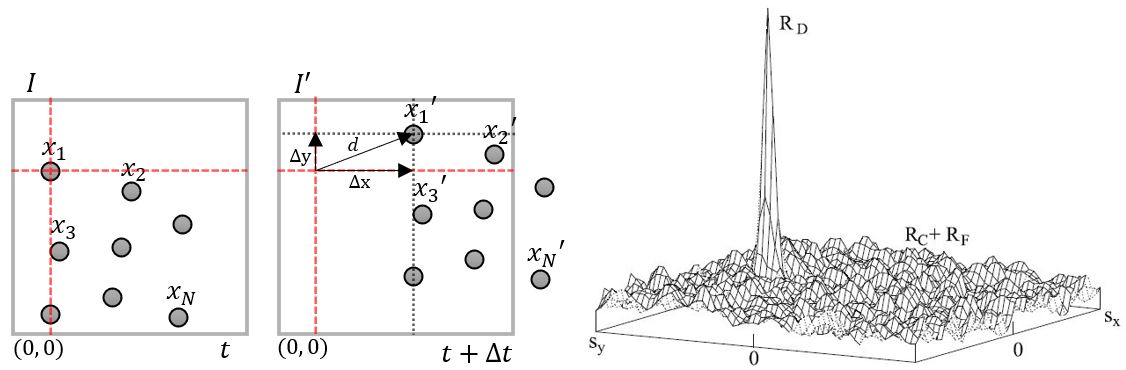
\includegraphics[width=16cm]{./3_MatPozadina/3_5KrosKorelacija.jpg} 
	\caption{Shema polja intenziteta $I$ i $I'$ u trenutcima $t$ i $t + \Delta t$ prikazana na prve dvije slike, te kompozicija vrhova korelacijske funkcije na trećoj slici \cite{raffel2018_book}}
	\label{sl:3.5}
\end{figure}
\par
Iz jednadžbe \ref{eqn:3.30} vidi se da pomak korelacije je funkcija nasumičnih varijabli $(\boldsymbol{X_{i}})_{i=1\dots N}$. Posljedično pomak je i sam nasumična varijabla i za različite izvedbe općenito istih uvjeta, dobit će se kvalitativno različite procjene pomaka koje ovise o stanju skupa čestica. Kako bi procjena pomaka u tom slučaju bila što bolja potrebno je izvesti pravila za generalnu optimizaciju procjene vrijednosti pomaka, što će biti prikazano u sljedećem poglavlju.
\FloatBarrier
\section{Očekivana vrijednost pomaka korelacije}
Kako bi se izvela pravila za opću procjenu pomaka odrediti će se očekivana vrijednost korelacijskog pomaka $E\{R_{D}\}$ za sve koncepte $\boldsymbol{\Gamma}$. Konkretnije, izračunati će se srednja korelacijska funkcija za sve moguće "uzorke" koji se mogu napraviti sa $N$ čestica. Iz jednadžbe \ref{eqn:3.30} slijedi:
\begin{equation}
	\begin{split}
		E\{R_{D}\} &= E\left\{R_{\tau}(\boldsymbol{s}-\boldsymbol{d})\sum_{i=1}^{N}V_{0}(\boldsymbol{X_{i}})\, V_{0}(\boldsymbol{X_{i}}+\boldsymbol{D})\right\}\\
		&=R_{\tau}(\boldsymbol{s}-\boldsymbol{d})\, E\left\{ \sum_{i=1}^{N}V_{0}(\boldsymbol{X_{i}})\, V_{0}(\boldsymbol{X_{i}}+\boldsymbol{D})\right\}
	\end{split}
	\label{eqn:3.31}
\end{equation}
Ako se zapiše $f_{l}(\boldsymbol{X})=V_{0}(\boldsymbol{X_{i}})\, V_{0}(\boldsymbol{X_{i}}+\boldsymbol{D})$:
\begin{equation*}
	E\{R_{D}\} = R_{\tau}(\boldsymbol{s}-\boldsymbol{d})\, E\left\{\sum_{i=1}^{N}f_{l}(\boldsymbol{X_{i}})\right\}
\end{equation*}
$\sum_{i=1}^{N}f_{l}(\boldsymbol{X_{i}})$ promatra se kao funkcija $N$ nasumičnih varijabli $\boldsymbol{X_{1}}, \boldsymbol{X_{2}},...\, \boldsymbol{X_{N}}$, te se zato može napisati:
\begin{equation}
	\begin{split}
		E\left\{\sum_{i=1}^{N}f_{l}(\boldsymbol{X_{i}})\right\} = \sum_{i=1}^{N}E\{f_{l}(\boldsymbol{X_{i}})\} = \sum_{i=1}^{N}\dfrac{1}{V_{F}}\int f_{l}(\boldsymbol{X_{i}})d\boldsymbol{X_{i}}\\
		\Rightarrow E\left\{\sum_{i=1}^{N}f_{l}(\boldsymbol{X_{i}})\right\} = \dfrac{N}{V_{F}}\int_{V_{F}}f_{l}(\boldsymbol{X})d\boldsymbol{X}
	\end{split}
	\label{eqn:3.32}
\end{equation}
gdje je $\int_{V_{F}} f_{l}(\boldsymbol{X})d\boldsymbol{X}$ volumenski integral
\begin{equation*}
	\int \int \int f_{l}(X, Y, Z)\, d\boldsymbol{X}d\boldsymbol{Y}d\boldsymbol{Z}
\end{equation*}
što konačno daje:
\begin{equation}
	E\{R_{D}\}= \dfrac{N}{V_{F}}R_{\tau}(\boldsymbol{s}-\boldsymbol{d})\int_{V_{F}}f_{l}(\boldsymbol{X})d\boldsymbol{X}
	\label{eqn:3.33}
\end{equation}
Kako je $N$ definiran kao ukupan broj svih čestica unutar fluida, tako i $V_{F}$ je interpretiran kao volumen fluida unutar kojeg su dodane čestice markeri. Prema gornjoj definiciji $f_{l}(\boldsymbol{X})$ u praktičnom smislu može se reći da integracija mora biti izvršena preko volumena koji se sastoji od volumena ispitivanja koji se nalaze na slikama dobivenim tijekom prve ili druge ekspozicije. Integral nad $f_{l}(\boldsymbol{X})$, drugim riječima može biti zapisan kao:
\begin{equation}
	\begin{split}
		\int_{V_{F}}f_{l}(\boldsymbol{X})d\boldsymbol{X}  &= \int I_{0}(Z)\, I_{0}(Z+D_{Z})dZ \times \int \int W_{0}(X,Y)\, W_{0}(X+D_{X},Y+D_{Y})dXdY \\
		&=\int_{V_{F}}V_{0}^{2}(\boldsymbol{X})d\boldsymbol{X}\dot F_{O}(D_{Z})F_{I}(D_{X},D_{Y})
	\end{split}
	\label{eqn:3.34}
\end{equation}
gdje su:
\begin{equation}
	F_{I}(D_{X},D_{Y})=\dfrac{\int \int W_{0}(X, Y)\, W_{0}(X+D_{X}, Y+D_{Y})dXdY}{\int \int W_{0}^{2}(X, Y)dXdY}
	\label{eqn:3.35}
\end{equation}
i
\begin{equation}
	F_{O}(D_{Z})=\dfrac{\int I_{0}(Z)\, I_{0}(Z+D_{Z})dZ}{\int I_{0}^{2}(Z)dZ}
	\label{eqn:3.36}
\end{equation}
Prema literaturi \cite{keane1992theory} $F_{I}$ je definiran kao faktor koji izražava unutar-ravninski gubitak parova. Konačno jednadžba \ref{eqn:3.33} ima oblik:
\begin{equation}
	E\left\{R_{D}(\boldsymbol{s}, \boldsymbol{D})\right\}=C_{R}R_{\tau}(\boldsymbol{s}-\boldsymbol{d})F_{O}(D_{Z})F_{I}(D_{X},D_{Y})
	\label{eqn:3.37}
\end{equation}
gdje je konstanta $C_{R}$ definirana kao:
\begin{equation*}
	C_{R}=\dfrac{N}{V_{F}}\int_{V_{F}}V_{0}^{2}(\boldsymbol{X})d\boldsymbol{X}
\end{equation*}
U 2D PIV-u gubitak korelacije zbog gibanja izvan ravnine ili neusklađenosti svjetlosne ravnine ima dva efekta. Prvi efekt je u tome da je smanjena vjerojatnost detekcije ispravnog vektora brzina. Drugo, povećana je nesigurnost u mjerenjima polja brzina. Valjanost originalne definicije $F_{O}$ prema \cite{keane1992theory} je limitirana na upotrebu identičnog intenziteta laserskog profila pri svakoj ekspoziciji. Kako se laserska ravnina prilikom prvog i drugog osvijetljenja obično razlikuje u širini i obliku, korištenje predložene definicije $F_{O}$ je limitirano u praksi. Kako bi se zaobišla ova limitacija, u literaturi \cite{scharnowski2017generalization} predložena je nova definicija $F_{O}$ koja točno predviđa gubitak korelacije za sve neusklađene svjetlosne ravnine, te također potvrđuje originalnu $F_{O}$ definiciju prilikom idealnih uvjeta. 

\chapter{EVALUACIJA PIV TOČNOSTI}
\label{chap:Poglavlje_4}
Kvaliteta točnosti PIV mjerenja određena je veličinom greške unutar samih mjerenja. Sveukupna greška mjerenja prilikom PIV analize je kombinacija širokog spektra aspekata koji idu od postavki samog setup-a mjerenja, snimanja pa sve do metoda evaluacije. Na \textit{Slici \ref{sl:4.1}} prikazani su neki od glavnih parametara koje je potrebno uzeti u obzir prilikom PIV mjerenja.
\begin{figure}[h]  
	\centering
	%\usepackage{graphicx}
	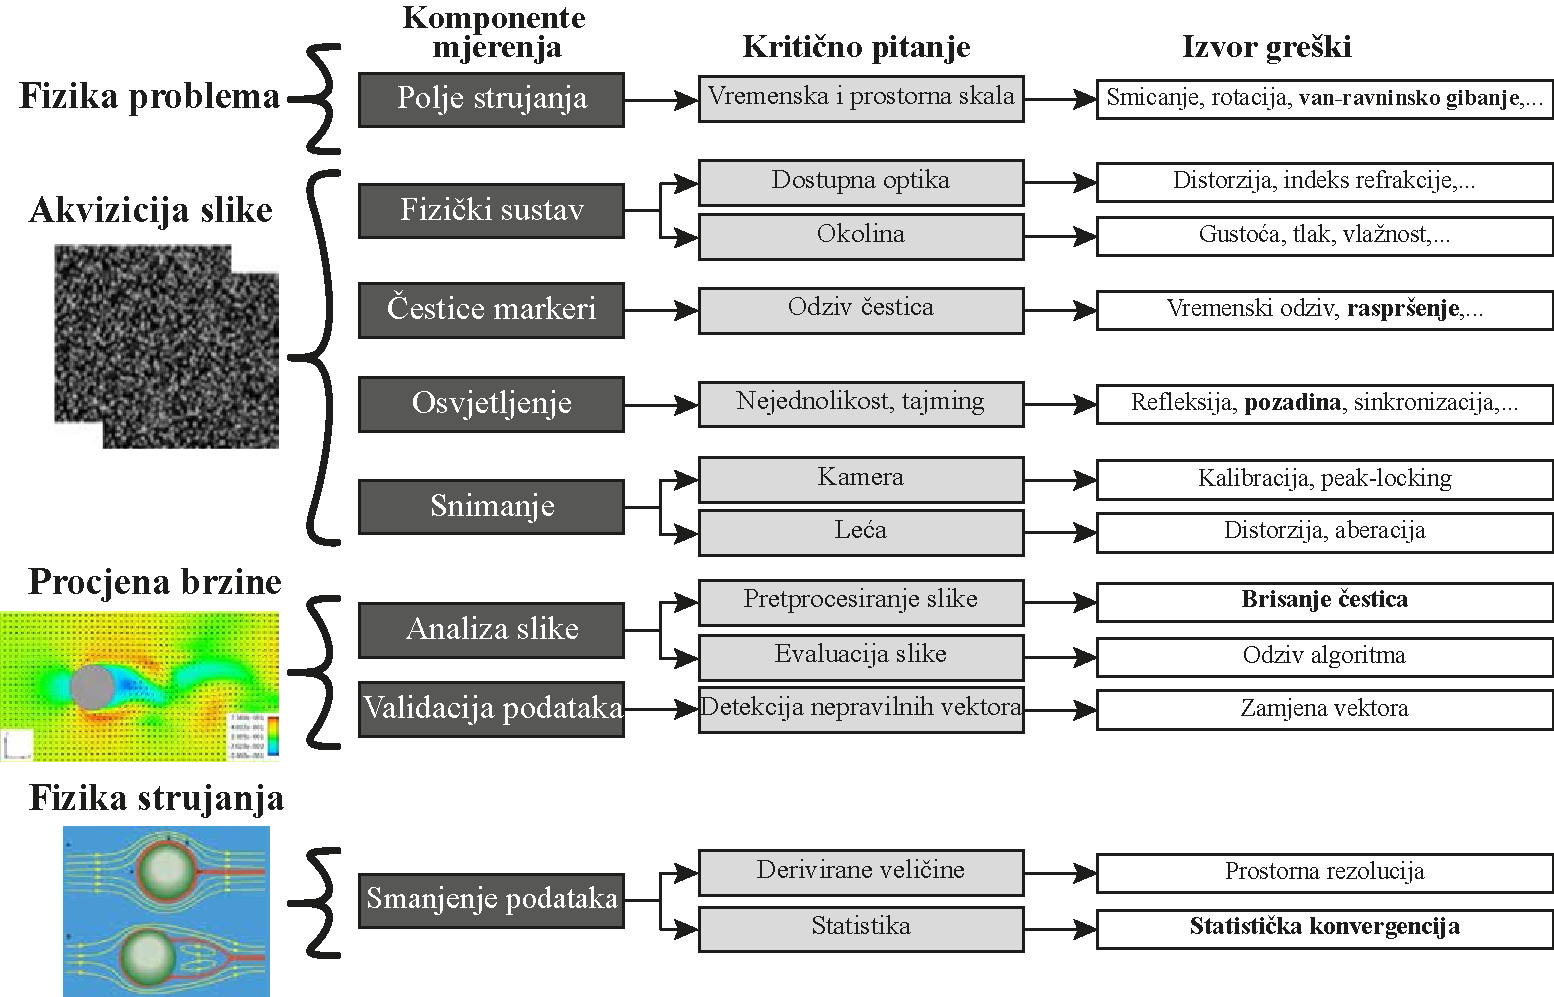
\includegraphics[width=16cm]{./4_PIVNesigurnost/slika4_1.pdf} 
	\caption{Kvantifikacija glavnih komponenti PIV mjerenja, te nekih od najvažnijih izvora pogrešaka (podebljane su greške koje se smatraju jako slučajne) \cite{sciacchitano2019_article}}
	\label{sl:4.1}
\end{figure}
\par
U DPIV analizi postoje dva glavna izvora nesigurnosti u mjerenjima: pristrana pogreška $\epsilon_{pristr.}$ i slučajna pogreška $\epsilon_{slu\textup{č}.}$ koji zajedno doprinose ukupnoj greški mjerenja $\epsilon$ \cite{raffel2018_book}. Pristrana pogreška određuje istinitost procjene pomaka. Istinitost je definirana kao "preklapanje" između srednje vrijednosti (velike količine) izmjerenih podataka te stvarnog pomaka. Slučajna pogreška određuje preciznost procjene pomaka. Preciznost se definira kao mjera veličine (širine) razmaka između procijenjenih pomaka. Moguće je da su mjerenja jako precizna, ali srednja vrijednost mjerenja nije točna jer se jako razlikuje od stvarnog pomaka (\textit{Slika \ref{sl:4.2}}). Istinitost i preciznost skupa definiraju točnost mjerenja PIV sustava. 
\begin{figure}[h]  
	\centering
	%\usepackage{graphicx}
	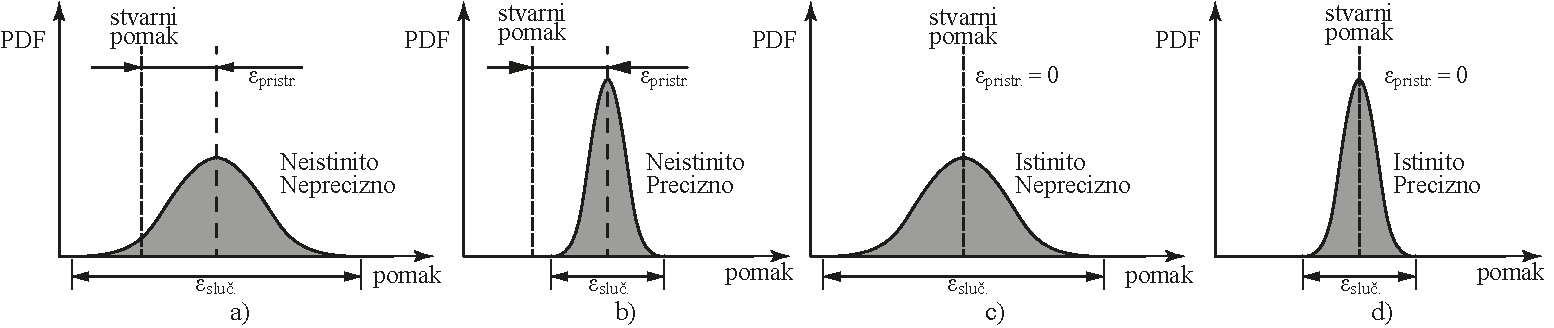
\includegraphics[width=16cm]{./4_PIVNesigurnost/slika4_2.pdf} 
	\caption{Definicija točnosti tj. istinitosti i preciznosti u PIV analizi}
	\label{sl:4.2}
\end{figure}
\par
Kod određivanja pristrane i slučajne pogreške, potreban je ogroman broj podataka i da bi rezultati bili relevantni potrebne su statističke simulacije koje upotrebljavaju veliki broj podataka (npr. Monte Carlo simulacija). Naravno, dodatno kako bi se odredila pogreška potrebno je znati i vrijednost stvarnog pomaka. Najjednostavniji način da se zadovolje ovi uvjeti je korištenje sintetičkih čestičnih slika (\textit{eng. synthetic particle images}), čija će upotreba biti kasnije objašnjena.  Pristrana pogreška računa se pomoću sljedeće formule:
\begin{equation}
	\epsilon_{pristr.}=\frac{1}{n}\sum_{i=1}^{n}x_{i} - x_{stv}
	\label{eqn:4.1}
\end{equation}
gdje $x_{i}$ predstavlja pomak izmjeren određenim DPIV algoritmom, dok je $x_{stv}$ stvarni pomak koji se generira u sintetičkoj slici.\\
Slučajna pogreška računa se putem izraza:
\begin{equation}
	\epsilon_{slu\textup{č}.}=\sqrt{\frac{1}{n}\sum_{i=1}^{n}(\overline{x}-x_{i})}
	\label{eqn:4.2}
\end{equation}
gdje $\overline{x}$ predstavlja srednju izmjerenu vrijednost pomaka, a $n$ broj čestica. Pristrana pogreška uzrokovana je tzv. peak-locking efektom koji postoji u većini kros-korelacijskih algoritama. Peak-locking (poznato i kao pristranost pixela) je ozbiljna pogreška pristranosti u PIV evaluaciji gdje izmjerene vrijednost lokacija i pomaka čestica su pristrana prema cjelobrojnim vrijednostima (integer). Do pogreške dolazi zbog "fittanja" glatke krivulje kroz diskretnu distribuciju intenziteta u korelacijskoj matrici tijekom pretraživanja korelacijskih vrhova. Pristrana pogreška je funkcija pomaka, veličina pogreške najviše ovisi o korelacijskom algoritmu, tehnici subpixelske aproksimacije, te promjeru čestice. U \textit{Tablici \ref{tab:4.1}} prikazano je testiranje nekoliko DPIV korelacijskih algoritama, te su na sljedećim slikama prikazani i rezultati točnosti testiranih algoritama uzimajući u obzir nekoliko eksperimentalnih situacija \cite{thielicke2014_phd} (sve simulacije su napravljene sa brojem čestica $n\geq 930 000$).
\begin{table}[h]
	\centering
	\caption{Testirani DPIV algoritmi (rezultati na \textit{Slikama \ref{sl:4.3} \ref{sl:4.4}, \ref{sl:4.5}}) \cite{thielicke2014_phd}}
	\resizebox{\textwidth}{!}{%
	\begin{tabular}{llllll}
		\hline
		\rowcolor[HTML]{C0C0C0} 
		\multicolumn{2}{l}{\cellcolor[HTML]{C0C0C0}\textbf{Parametar}} & \textbf{DKK}           & \textbf{DFT}           & \textbf{DFT multi-linearni} & \textbf{DFT multi-spline} \\ \hline
		\multicolumn{2}{l}{CLAHE, veličina {[}px{]}}                   & $50$                   & $50$                   & $50$                        & $50$                      \\
		\multicolumn{2}{l}{DPIV tehnika}                               & DKK                    & DFT                    & DFT                         & DFT                       \\
		\multicolumn{2}{l}{Subpixelska aproksimacija}                  & Gauss $3$-točke & Gauss $3$-točke & Gauss $3$-točke      & Gauss $3$-točke    \\
		\multicolumn{2}{l}{Deformacija prozora ispit.}                 & -                      & -                      & linearna                    & spline                    \\
		\multicolumn{2}{l}{Preklapanje {[}\%{]}}                       & $50$                   & $50$                   & $50$                        & $50$                      \\
		1. prolaz:          & Veličina proz. ispit. {[}px{]}          & $16\cdot 16$           & $16\cdot 16$           & $64\cdot 64$                & $16\cdot 16$              \\
		2. prolaz:          & Veličina proz. ispit. {[}px{]}          & -                      & -                      & $32\cdot 32$                & $16\cdot 16$              \\
		3. prolaz:          & Veličina proz. ispit. {[}px{]}          & -                      & -                      & $16\cdot 16$                & $16\cdot 16$              \\
		4. prolaz:          & Veličina proz. ispit. {[}px{]}          & -                      & -                      & -                           & $16\cdot 16$              \\ \hline
	\end{tabular}}
	\label{tab:4.1}
\end{table}
\par
Subpixelska aproksimacija također teži cjelobrojnim vrijednostima, a taj efekt postaje sve gori kada su čestice jako malene veličine. Snimke u kojima su čestice manje od 3 pixela daju jako uske vrhove u korelacijskoj matrici, što dovodi do toga da aproksimacija Gauss-ovom funkcijom se ne može izvršiti. Opisani problem može se vidjeti na \textit{Slici \ref{sl:4.3}}. Ovdje, svi testirani DPIV algoritmi imaju značajan nedostatak točnosti, zbog toga što se svi oslanjaju na  subpixelsku aproksimaciju u $3$ točke koja očito nije prikladna za snimke sa vrlo malenim česticama. Nadalje vidljiv je značajan pad vrijednosti greške za snimke sa promjerom čestice od 3 mm (\textit{Slika \ref{sl:4.4}}), te 5 mm (\textit{Slika \ref{sl:4.5}})
\begin{figure}[h]  
	\centering
	%\usepackage{graphicx}
	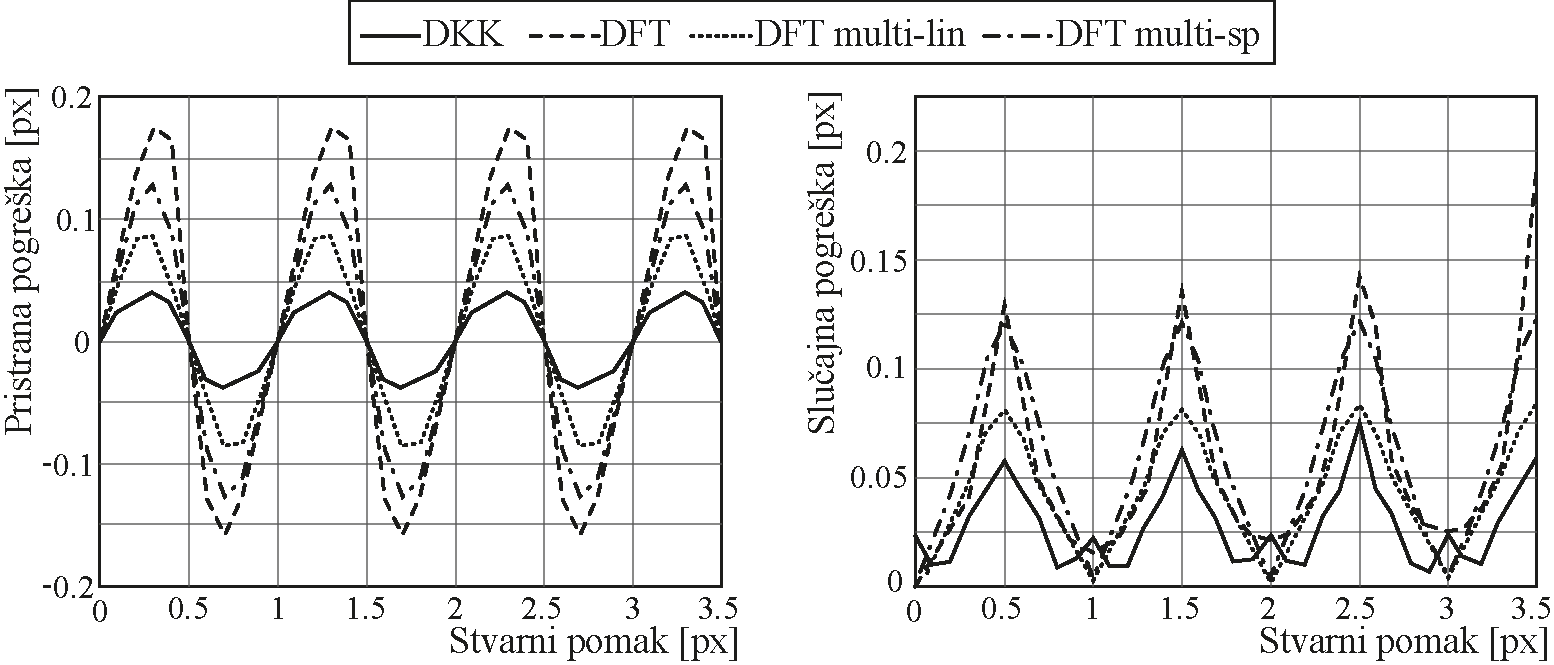
\includegraphics[width=16.5cm]{./4_PIVNesigurnost/slika4_3.pdf} 
	\caption{Pristrana i slučajna pogreška za čestice markere promjera 1 pixel}
	\label{sl:4.3}
\end{figure}
\begin{figure}[h]  
	\centering
	%\usepackage{graphicx}
	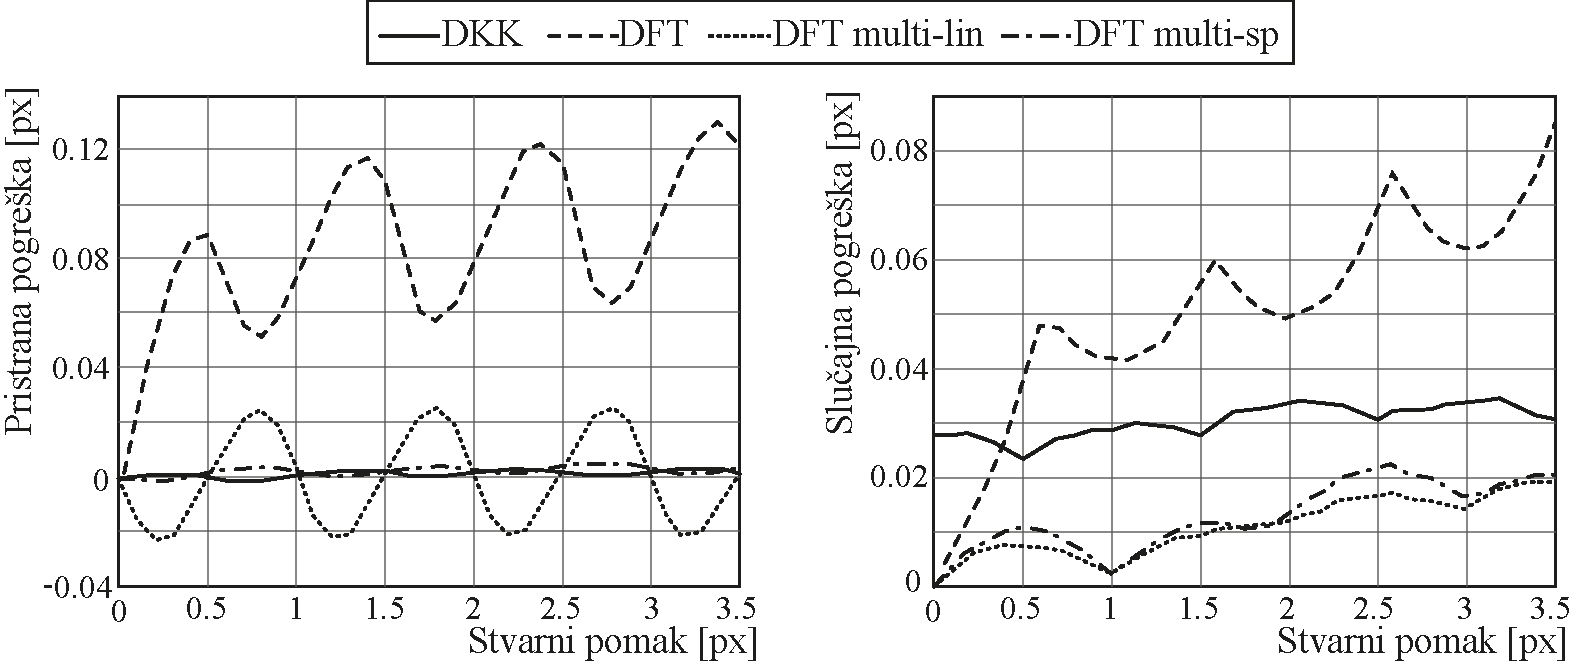
\includegraphics[width=16.5cm]{./4_PIVNesigurnost/slika4_4.pdf} 
	\caption{Pristrana i slučajna pogreška za čestice markere promjera 3 pixel-a}
	\label{sl:4.4}
\end{figure}
\begin{figure}[h]  
	\centering
	%\usepackage{graphicx}
	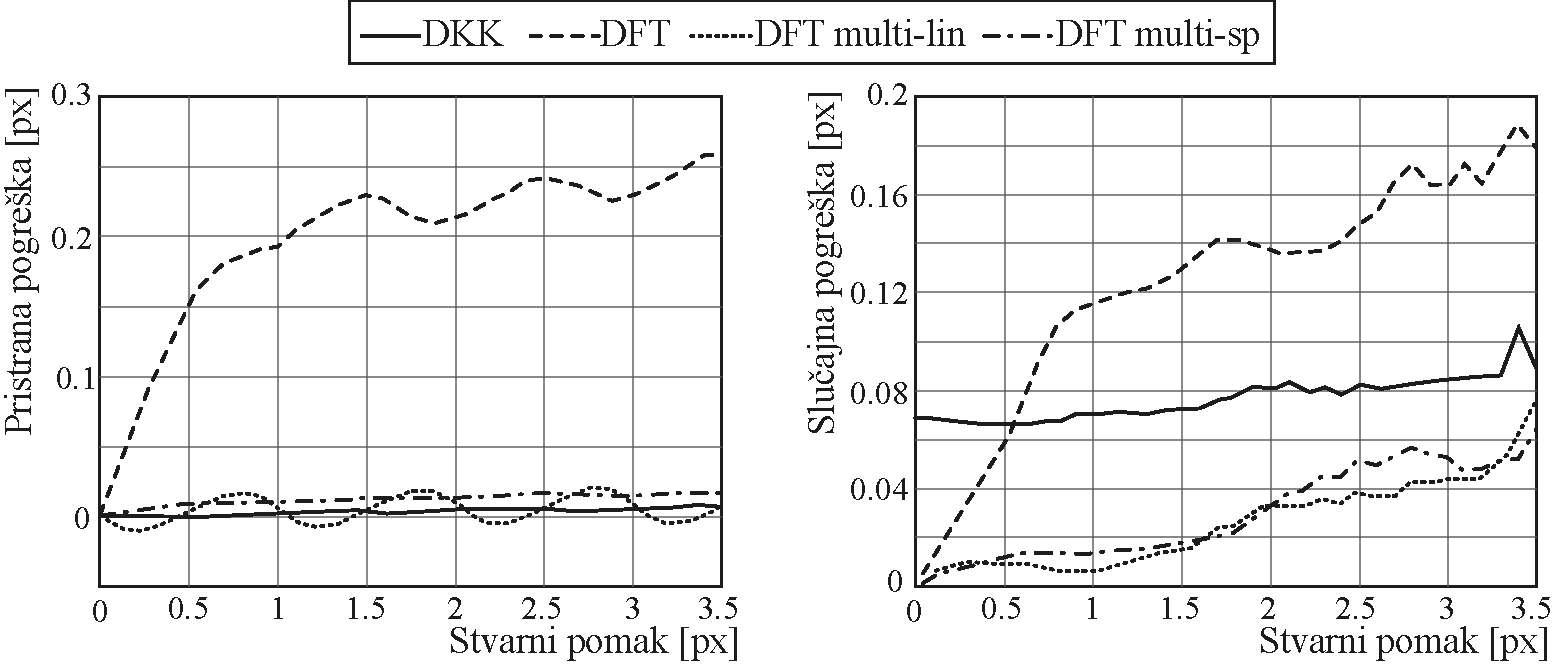
\includegraphics[width=16.5cm]{./4_PIVNesigurnost/slika4_5.pdf} 
	\caption{Pristrana i slučajna pogreška za čestice markere promjera 5 pixel-a}
	\label{sl:4.5}
\end{figure}
\FloatBarrier
\section{Dinamički raspon brzina ($DVR$) i dinamički prostorni raspon ($DSR$)}
Tipična točnost PIV mjerenja brzine je unutar 1\%, dok je prostorna rezolucija unutar 1 milimetra \cite{adrian1997dynamic}. Korisnost PIV mjerenja obično je karakterizirana sa svojom točnosti i prostornom rezolucijom. Međutim, nijedna od ovih veličina ne opisuje kompletno sposobnosti PIV sustava, te se zbog toga koriste pojmovi dinamički raspon brzine $DVR$ (\textit{eng. Dynamic Velocity Range}) i dinamički prostorni raspon $DSR$ (\textit{eng. Dynamic Spatial Range}). Dinamički raspon brzina definiran je kao omjer maksimalne brzine $U_{max}$ (koji se može mjeriti sa određenim postavkama PIV sustava) sa minimalnom razlučivosti fluktuacija mjerenih brzina $\sigma_{U}$ (srednji kvadratni korijen pogrešaka brzine), tj. jednostavnije omjerom maksimalne i minimalne razlučive brzine:
\begin{equation}
	DVR=\frac{U_{max}}{\sigma_{U}}
	\label{eqn:4.3}
\end{equation}
U svojim počecima PIV sustavi imali dosta niske vrijednosti $DVR$ (u rasponu 10-100), te zbog toga razloga mjerenja nisu mogla razlučiti određene dijelove strujanja u slučaju da je dolazilo do značajnih promjena brzine. Čak i ako nije bilo velikih varijacija brzine, nizak raspon $DVR$ dovodio je do toga de je trebalo oprezno prilagoditi parametre mjerenja da brzine strujanja upadnu u zadano područje. Dinamički prostorni raspon ili raspon skala definira se kao omjer vidnog polja čestica i najmanje razlučive prostorne varijacije, tj. može se shvatiti kao veličina koja govori o tome koliko je moguće mjerenje najmanjih skala strujanja (npr. granični sloj) uključenih unutar većih skala strujanja:
\begin{equation}
	DSR=\frac{x_{max}}{D_{I}}
	\label{eqn:4.4}
\end{equation} 
gdje je $x_{max}$ duljina senzora kamere u pixelima, a $D_{I}$ duljina prozora ispitivanja također u pixelima. Kako bi se kompenzirao gubitak informacija unutar malenih skala strujanja moguća je opcija uvećati optičko povećanje sustava snimanja $M_{0}$ ili dodatno povećati koncentraciju čestica markera u protoku. Na taj način mjerena nesigurnost može biti smanjena na račun manjeg vidnog polja strujanja, što će naravno dovesti do toga da se izgube veće skale strujanja koje su i prvotno bile od veće zanimljivosti.
\par
U današnje vrijeme, mnogo snažniji laseri, osjetljive digitalne kamere, te sofisticirane analize snimki i dobivenih vektora i brzina, uz sve bolje metode ubacivanja čestica markera dovele su do toga da PIV mjerenja budu znatno pouzdanija. Međutim i dalje ostaje veliki problem PIV mjerenja sa niskom nesigurnošću, zbog toga što je iznimno složeno podešavanje parametara sustava koji se ne mogu mijenjati individualno, zbog velike ovisnosti jednih o drugima. Prema tome i dalje je veoma važno poznavanje osnovnih znanja i mogućnosti kako PIV sustava, tako i same fizike strujanja.
\section{Generiranje sintetičkih PIV snimki}
Kako slučajna i pristrana pogreška u digitalnoj PIV evaluaciji mogu biti jedino poznate ako su točno poznati i stvarni pomaci čestica, potrebno je poznavati iznose pomaka. U početku su s koristile PIV snimke iz izrazito mirnih strujanja u kojima su sa velikom sigurnošću bile poznate veličine i karakteristike strujanja. Sa tim poznatim i određenim karakteristikama mogli su se testirati i kalibrirati određeni PIV softveri, tj. korelacijski signali koji u najvećoj mjeri doprinose mjernoj nesigurnosti. Međutim, svaki put kada bi se trebalo raditi drugačije mjerenje bilo je potrebno napraviti i nove posebne kalibracije gdje se svaki parametar mora oprezno provjeriti, što je izrazito neefikasan i spor proces. Jedan od pristupa je korištenje umjetno stvorenih (sintetičkih) PIV snimki koje bi zajedno sa numeričkom simulacijom (Monte Carlo) uspješno mogle ispitati valjanost PIV softvera. Procjena nesigurnosti bazirana na sintetičkim snimkama pruža tri glavne prednosti:
\begin{enumerate}[label=\textbf{\arabic*)}, leftmargin=*, align=left, itemsep=0em, topsep=0em]
	\item Moguća je potpuna kontrola parametara koji se koriste u simulaciji (nasuprot eksperimentima gdje postoji mnogo nesigurnosti kao što su: lokalna gustoća, temperatura, viskoznost, čestica unutar okoline, razni problemi za kamerom i osvjetljenjem).
	\item Moguća je individualna kontrola parametara, što je nemoguće postići u eksperimentima zbog međusobne ovisnosti.
	\item Raspon mijenjanja vrijednosti parametara može biti povećan ili smanjen čak i izvan granica raspona koje je eksperimentalno moguće postići.
\end{enumerate}
Glavni nedostatak ovom pristupu je u tome da ipak nije moguće simulirati sve moguće fizičke efekte koji se pojavljuju u strujanju, te simulirane snimke mogu biti prejednostavne.
\par
Sintetičke slike su generirane u PIVlab softveru po preporukama u literaturi \cite{raffel2018_book}, te čestice unutar njih moraju zadovoljiti određene karakteristike: promjer, oblik, prostornu gustoću, dubinu slike, itd.. Sve čestice imaju Gauss-ov profil intenziteta sa točno određenim promjerom koji je zadan jednadžbom (\ref{eqn:4.5}). 
\begin{equation}
	I(x, y) = I_{0} \exp\left(\frac{-(x-x_{0})^{2}-(y-y_{0})^{2}}{\frac{1}{8}d_{\tau}^{2}}\right)
	\label{eqn:4.5}
\end{equation}
gdje $x_{0}$ i $y_{0}$ predstavljaju sredinu lokacije čestice, $I_{0}$ vrijednost intenziteta u sredini čestice (najveća vrijednost), te $d_{\tau}$ promjer čestice. Faktor $I_{0}$ također je u funkciji pozicije čestice u smjeru Z-osi, kako bi se uzela u obzir debljina laserske zrake (\textit{Slika \ref{sl:4.6} lijevo}). Poznati broj čestica je slučajno postavljen, te simulirana laserska zraka također ima Gauss-ov profil intenziteta (jednadžba \ref{eqn:4.6}) kako bi se u obzir uzele 3D lokacije čestica u stvarnosti (\textit{Slika \ref{sl:4.6}}). 
\begin{equation}
	I_{0}(Z)=q\exp \left( -\frac{1}{\sqrt{2\pi}} \left|\frac{2Z^{2}}{\Delta Z_{0}^{2}}\right|^{s} \right)
	\label{eqn:4.6}
\end{equation}
gdje $q$ predstavlja efikasnost kojom čestice raspršuju obasjanu svjetlost, $\Delta Z_{0}$ predstavlja debljinu svjetlosne zrake na kojoj intenzitet opada na $-\frac{1}{\sqrt{2\pi}}\approx0.67$ maksimalnog intenziteta koji se nalazi u sredini zrake ($Z=0$), a $s$ je faktor oblika profila (za $s=2$ profil intenziteta ima oblik Gauss-ove funkcije, dok za veće vrijednosti poprima oblik tzv. top-hat funkcije kako je prikazano na \textit{Slika \ref{sl:4.6} desno}). Nadalje, pretpostavlja se da promjer čestica $d_{\tau}$ je mnogo manji od debljine laserske zrake $\Delta Z_{0}$. Generiranje sintetičke slike se vrši na način da se prvo generira slučajni broj koji specificira lokaciju čestice ($x_{0}, y_{0}, z_{0}$) unutar 3D laserske zrake (\textit{Slika \ref{sl:4.6} lijevo}). Maksimalni intenzitet $I_{0}(z_{0})$ se odredi uz pomoć jednadžbe \ref{eqn:4.6}. Nakon čega se ta vrijednost uvrsti u jednadžbu \ref{eqn:4.5} gdje se izračuna vrijednost intenziteta svijetla koju uhvati svaki pixel. Naknadno je moguće dodavanje raznih šumova koji bi još opisali dodatno uvjete prilikom stvarnog PIV mjerenja (npr. šum senzora kamere).
\begin{figure}[h]  
	\centering
	%\usepackage{graphicx}
	\includegraphics[width=13cm]{./4_PIVNesigurnost/slika4_6.jpg} 
	\caption{3D prostor laserske zrake sa generiranim sintetičkim česticama (lijevo), te funkcije kojima je moguće opisati profil intenziteta laserske svjetlosti prema jednadžbi \ref{eqn:4.5} (desno)\cite{raffel2018_book}}
	\label{sl:4.6}
\end{figure}
\par
Kako bi se generirala sljedeća slika, to jest pomak čestica, obično se koriste neka od generičkih strujanja koja se dobiju analitički (osnovana laminarna strujanja) ili numerički (turbulentno) te se na osnovi njihovih rješenja generiraju nove slike sa pomaknutim česticama.
\FloatBarrier
\section{Utjecajni parametri na korelacijski signal}
U ovom potpoglavlju ukratko će biti objašnjeni utjecaji nekih od parametra koje je moguće kontrolirati pri generiranju sintetičkih snimki, a koji značajno utječu na točnosti DPIV algoritama. Variranjem jednog po jednog od ovih parametara omogućava određivanje osjetljivosti, te samim time i optimizaciju kasnijeg eksperimentalnog postupka:
\begin{description}[style=unboxed,leftmargin=0cm]
	\item[Promjer čestica markera] Veličina čestica u PIV eksperimentima obično dosta varira, te značajno utječe na točnost analize. U literaturama \cite{guezennec1990statistical} ustanovljen je pad točnosti DPIV analize za čestice koje imaju promjer veći od 2 pixela, te je pronađen optimalni promjer od 1.5 pixela\cite{raffel2018_book}. Također jačina utjecaja promjera čestice ovisi i o korištenom DPIV algoritmu (\textit{Slika \ref{sl:4.7}}). Na slici je vidljivo kako slučajne pogreške za DKK i obični DFT algoritam imaju lokalni minimum na promjeru od 1.8-2 pixela. Dok je za DFT sa tehnikama deformacije prozora ispitivanja minimum pomaknut udesno, te se vidi kako ovi algoritmi imaju značajno manji iznos slučajne pogreške.
	\begin{figure}[H]  
		\centering
		%\usepackage{graphicx}
		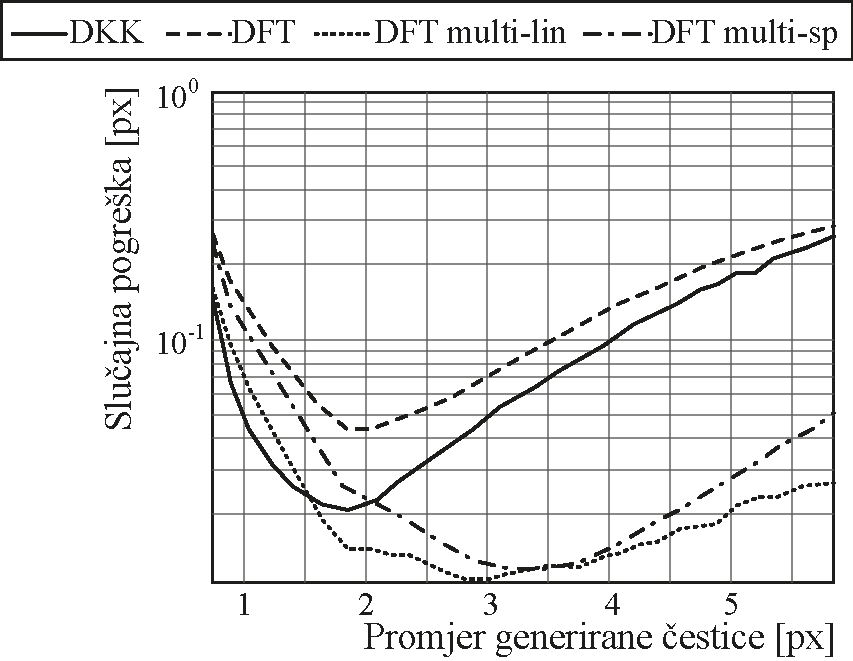
\includegraphics[width=10cm]{./4_PIVNesigurnost/slika4_7.pdf} 
		\caption{Efekt veličine promjera čestica na slučajnu pogrešku za prosječni pomak čestica od 3.5 pixela \cite{thielicke2014_article}}
		\label{sl:4.7}
	\end{figure}
	\item[Gustoća distribucije čestica] Kako su čestice nosioci informacije u PIV snimkama, gustoća njihove distribucije jako je bitna za dobru kvalitetu mjerenja. Vjerojatnost detekcije ispravnog pomaka znatno je veća ako je broj čestica unutar prozora ispitivanja oko 5. Broj uhvaćenih parova čestica u prozoru ispitivanja najviše ovisi o 3 faktora: gustoći čestica u snimci, količini pomaka koji se dogode unutar laserske ravnine, te količini pomaka izvan laserske ravnine (\textit{eng. out-of-plane motion}). 
	\item[Šum foto-senzora] Neželjeni šum na snimkama također smanjuje točnost mjerenja, a uzrokovan je ne-idealnom pretvorbom fotona električni signal na foto-senzoru. Jačina šuma ovisi o izvedbi senzora (CMOS ili CCD), te kvaliteti senzora. Analizu efekta šuma na točnost DPIV-a moguće je provjeriti dodavanjem umjetnog tzv. Gauss-ovog šuma (normalno distribuirani šum) u snimku. Ustanovljeno je kako obični DFT algoritam značajno gubi na točnosti zbog dodanog šum, dok DKK i DFT sa tehnikama deformacija prozora ispitivanja se mogu nositi sa šumom na snimkama.
	\item[Gubitak čestica unutar volumena ispitivanja (\textit{eng. out-of-plane motion})] U 2D DPIV analizi gubitak parova povezanih čestica je neizbježan zbog (uvijek) prisutnog 3D strujanja. Izgubljene čestice dovode do gubitka informacije, te samim time i povećane nesigurnosti zbog gubitka korelacijskog signala. Ovaj efekt moguće je simulirati na način da se umjetnim snimkama slučajno oduzme dio čestica na različitim pozicijama. U literaturi \cite{thielicke2014_phd} ustanovljeno je kako DFT algoritam ponovno dosta slabije reagira na gubitak čestica u odnosu na ostale.
	\item[Zamućenje pokreta] Uzrokovano je predugom ekspozicijom u kojoj dolazi do prebrzog kretanja čestica. Za vrijeme ekspozicije čestica se giba prevelikom brzinom te senzor kamere ne hvata trenutačno  njenu svjetlost, nego dobiva svjetlost čestice u više pozicija, zbog čega dolazi do zamućenja slike. Rješenje u vidu kraćeg trajanja ekspozicije, gdje se želi zamrznuti gibanje, često nije moguće zbog toga što onda premalo svjetlosti ulazi u senzor kamere. Zamućene slike iskrivljuju korelacijske vrhove, te tako povećavaju nesigurnost PIV analize. Efekt zamućenja slike, te koliku količinu nesigurnosti unosi u mjerenje može se simulirati tako da se umjetna slika konvoluira sa jednodimenzionalnim filtrom. DFT sa tehnikama deformacije prozora dosta su robusni, te su do određene mjere otporni i na ovaj utjecaj, dok obični DFT i DKK imaju povećanu nesigurnost.
	\item[Smicanje] U opisu tehnika deformacije prozora, predstavljen je otežavajući efekt smicanja unutar prozora ispitivanja. Opisana tehnika donekle limitira negativan utjecaj smicanja na točnost PIV analize. Smicanje se može simulirati primjenom kosog pomaka mreže snimke, te je u litraturi \cite{thielicke2014_phd} ustanovljeno kako obični DFT algoritam jako loše reagira na smicanje, DKK algoritam daje malo bolje rezultate, ali i dalje nedovoljno dobro kao algoritmi koji imaju uključene tehnike deformacije prozora, najveća točnost ostvarena je sa DFT algoritmom koji sadrži tehniku deformacije prozora, a koristi spline interpolaciju. 
\end{description}
\chapter{PIVlab PROGRAMSKI PAKET}
\label{chap:Poglavlje5}

U današnje vrijeme primjena PIV mjerenja postala je sve češća, te je PIV gotovo implementiran u svako područje dinamike fluida gdje brzine i pomaci trebaju biti kvantificirani, od istraživanja do razvoja. U te svrhe na tržištu su se pojavili brojni komercijalni PIV softveri (npr. Dantec DynamicStudio, ILA PIVview, LaVision Flowmaster, TSI INSIGHT), koji često nisu limitirani samo na 2D PIV mjerenja, nego u svoje sučelje imaju uključena i 3D (stereo) mjerenja, te još napredniju obrade podataka (volumetrijski PIV). Također postoje i brojni open-source PIV softveri ( JPIV\cite{jpiv}, Fluidimage\cite{fluidimage}, Fluere\cite{fluere}, mpiv\cite{mpiv}, UVMAT\cite{uvmat}, OpenPIV\cite{openpiv}) koji se isto tako mogu koristiti u znanstvene svrhe.
\par
U ovom radu koristi se open-source PIVlab\cite{thielicke2021PIVinMatLab} softver koji je prvotno objavljen 2010 godine, te se aktivno održava i ažurira i danas.  PIVlab je implementiran kao besplatni toolbox i aplikacija u programski jezik MATLAB. Na \textit{Slici \ref{sl:5.1}} prikazan je dijagram toka rada i opcija koje nudi PIVlab sučelje. Sa slike je vidljivo kako PIV analiza započinje sa učitavanjem snimki (ulaz), te završava sa "izbacivanje" izlaznih podataka. U ovom poglavlju ukratko će biti objašnjene i prikazane većina opcija i koje PIVlab nudi. Obično se cjelokupna analiza izvršava u PIVlab grafičkom sučelju (PIVlab\_GUI.m), no moguća je kontrola i bez sučelja koristeći command-line.
\begin{figure}[h]  
	\centering
	%\usepackage{graphicx}
	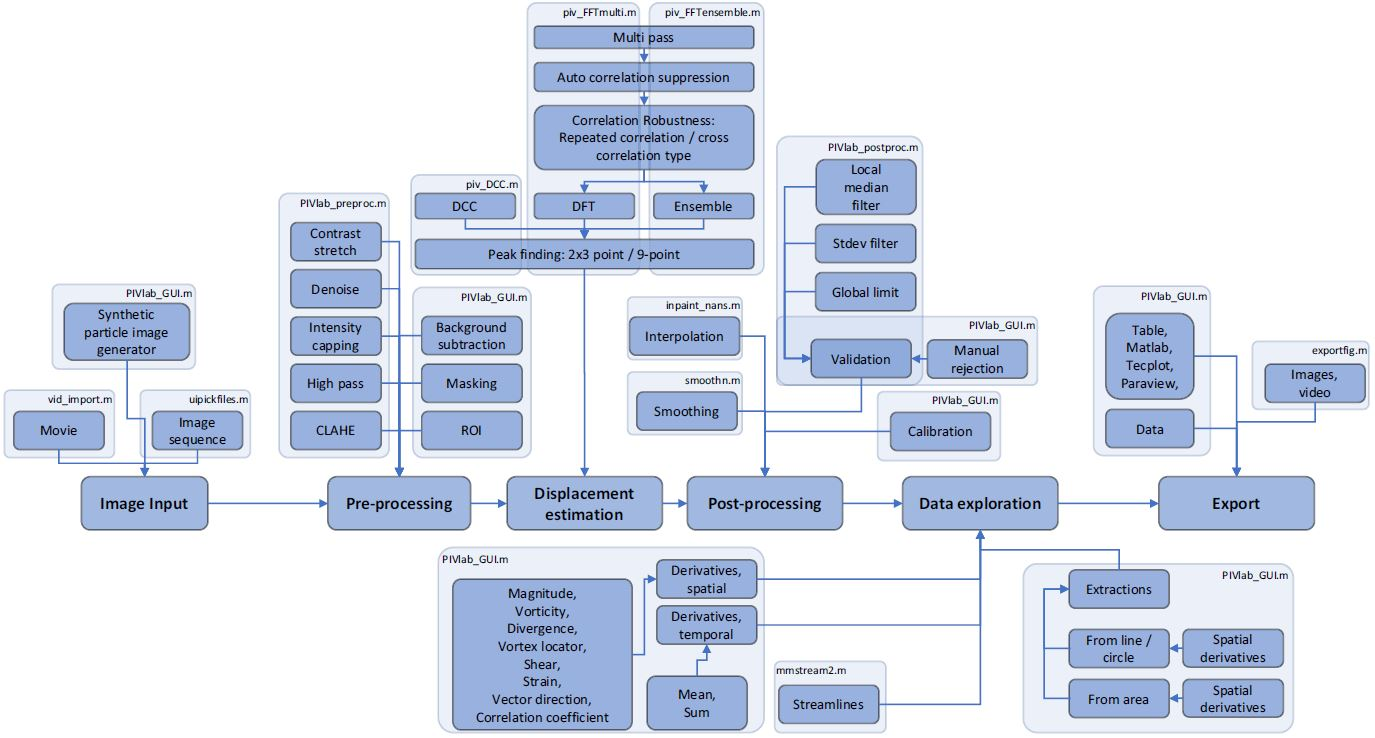
\includegraphics[width=16.6cm]{./5_PIVlab/slika5_1.jpg} 
	\caption{Arhitektura i dijagram toka PIVlab-a \cite{thielicke2021PIVinMatLab}}
	\label{sl:5.1}
\end{figure}
\par
U najnoviju verziju PIVlab softvera implementirana su brojna poboljšanja. U nastavku će samo neka bitnija poboljšanja biti ukratko objašnjena radi lakšeg razumijevanja načina rada softvera.
\begin{description}[style=unboxed,leftmargin=0cm]
	\item[Korelacija skupine snimki (\textit{eng. ensemble correlation})] Pristup korelacija skupine snimki PIV mjerenjima temelji se na usrednjavanju korelacijskih matrica svih dostupnih snimki prije nego što nastupi pronalazak korelacijskog vrha, te sama procjena srednjeg pomaka čestica. Generalno ova tehnika procesiranja koristi se najviše u PIV mjerenjima gdje je gustoća distribucija čestica markera mala (npr. $\mu$PIV). Usrednjavanjem matrica dobije se konačna korelacijska matrica (\textit{Slika \ref{sl:5.2}}) u kojoj je omjer signal-šum mnogo bolji odnosno veći. Veliki nedostatak ovog pristupa je taj što strujanje mora biti stacionarno, tj. ne smije se mijenjati u vremenu, što je i logično jer tada bi imali različite brzine u različitim trenucima snimki, što bi rezultiralo u proširenom korelacijskom vrhu čija detekcija bi bila neuspješna.
	\begin{figure}[H]  
		\centering
		%\usepackage{graphicx}
		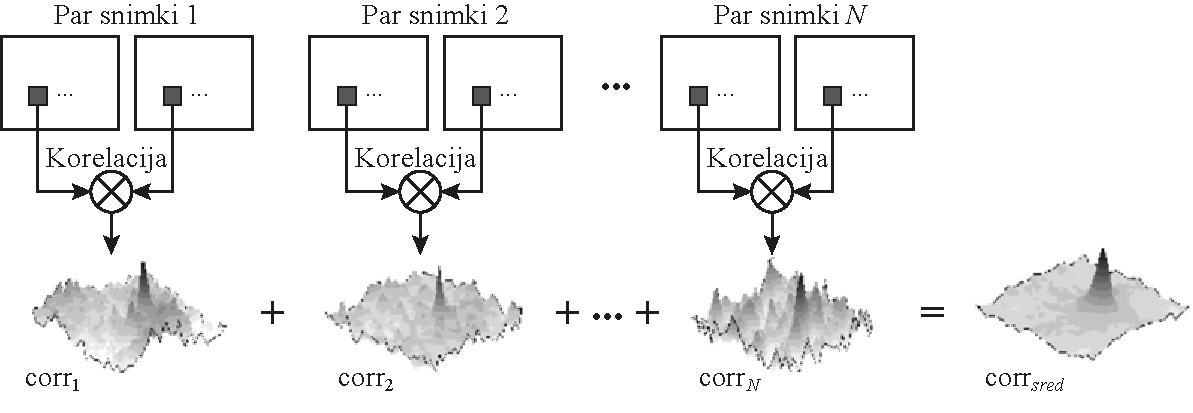
\includegraphics[width=16cm]{./5_PIVlab/slika5_2.pdf} 
		\caption{Koncept pristupa adaptivnoj korelaciji skupine snimki \cite{willert2008ensemble}}
		\label{sl:5.2}
	\end{figure}
	Na \textit{Slici \ref{sl:5.2}} jasno je uočljiva velika prednost ove tehnike, naime na posljednjoj usrednjenoj korelacijskoj ravnini vidljiv je značajan gubitak šuma nego na svakoj korelaciji posebno.
	\item[Poboljšanje korelacijskoj algoritma - kružna i linearna korelacija] PIVlab ima mogućnost primjene direktne kros-korelacije (DKK) u prostornoj domeni, te kros-korelacije signala u frekvencijskoj domeni koristeći diskretnu Fourierovu transformaciju (DFT). DFT algoritam je 30 do 50\% brži od DKK ovisno o implementaciji. PIVlab tipično koristi kružnu kros-korelaciju kako bi izveo DFT, kružna kros-korelacija pretpostavlja kako je signal periodičan, što naravno nije realan slučaj, te radi toga ova pretpostavka unosi frekvencije u DFT spektar koje inače ne postoje\cite{raffel2018_book}. Kako bi se izbjegao ovaj negativan učinak, signal može biti nuliran na granicama, što dovodi do linearne, ne-periodične kros-korelacije. Kako tipični podaci u snimkama imaju određeni šum (pozadinski signal koji različit od nule), nuliranje dovodi od rubnog diskontinuiteta, koji ponovno uništava spektar DFT analize i kros-korelacijski signal. Efekt "oštrih rubova" može biti oslabljen oduzimanjem prosječne vrijednosti intenziteta iz ulaznih snimki.
	\item[Poboljšanje korelacijskog algoritma - ponovljena korelacija] Još jedna tehnika da se dobije robusnija kros-korelacija je "ponavljanje korelacije". Ova metoda služi kao "ne-naknadno ispitivanje" kako bi se smanjio broj nepravilno dobivenih vektora brzine. Naime ova tehnika poboljšava dobivanje podataka kod snimki sa lošim omjerom signal-šuma, kros-korelacija se ne izvršava samo jednom za svaku procjenu pomaka, nego ukupno pet puta. Prozori ispitivanja se pomiču, gore-lijevo, gore-desno, dolje-lijevo i dolje-desno za 25\% duljine prozora ispitivanja. Dobivene korelacijske matrice se potom množe, što rezultira u novoj matrici koja ima manje šuma, te više izraženim vrhovima. Svaka korelacijska vrijednost koja nije prisutna u samo jednoj od pet korelacijskih matrica tako je izbačena iz konačne korelacijske matrice. Osnovne opcije koje sadrži PIVlab softver prikazane su u \textit{Tablici \ref{tab:5.1}}, naravno ove opcije se mogu i dodatno naštimati, ali za prosječnu analizu dovoljne su zadane tri postavke.
	\begin{table}[h]
		\centering
		\caption{Osnovne postavke korelacijskog algoritma u PIVlabu \cite{thielicke2021PIVinMatLab}}
		\begin{tabular}{|l|llll|}
			\hline
			\rowcolor[HTML]{C0C0C0} 
			{\color[HTML]{000000} \textbf{\begin{tabular}[c]{@{}l@{}}Robusnost \\ korelacije\end{tabular}}} & {\color[HTML]{000000} \textbf{\begin{tabular}[c]{@{}l@{}}Tehnika \\ deformacije \\ prozora\end{tabular}}} & {\color[HTML]{000000} \textbf{\begin{tabular}[c]{@{}l@{}}Kros-\\ korelacija\end{tabular}}} & {\color[HTML]{000000} \textbf{\begin{tabular}[c]{@{}l@{}}Ponovljena \\ korelacija\end{tabular}}} & {\color[HTML]{000000} \textbf{\begin{tabular}[c]{@{}l@{}}Vrijeme \\ izvršenja\end{tabular}}} \\ \hline
			\textbf{"Standard"}                                                                              & linearna                                                                                                  & kružna                                                                                     & isključeno                                                                                       & +                                                                                            \\
			\textbf{"High"}                                                                                  & spline                                                                                                    & linearna                                                                                   & isključeno                                                                                       & ++                                                                                           \\
			\textbf{"Extreme"}                                                                               & spline                                                                                                    & linearna                                                                                   & uključeno                                                                                        & ++++                                                                                         \\ \hline
		\end{tabular}
	\label{tab:5.1}
	\end{table}
	\item[Eliminacija pozadine] Neravnomjerno osvjetljenje, te ostali mogući pozadinski efekti u snimkama mogu rezultirati dodatnom procjenom nepravilnih vektora. Ovaj neželjeni efekt gdje pozadina daje visok postotak šuma u korelacijskoj ravnini može biti eliminiran na način da se izračuna prosječna vrijednost svih dostupnih snimki te da se dobivena vrijednost oduzme od svake snimke posebno.
	\item[Potiskivanje auto-korelacije] Još jedna od metoda poboljšanja PIV mjerenja je potiskivanje stacionarnog pozadinskog signala u korelaciji. Kao što je već ranije objašnjeno auto-korelacija je množenje snimke same sa sobom, što rezultira nepostojanjem pomaka. U ovom slučaju do auto-korelacije dolazi (iako su korelirane dvije različite snimke) zbog toga što pozadinski signal (šum) dominira nad korelacijom, a dostupan je samo jedan par snimki, te tada korištenje eliminacije pozadine nije moguće. U tom slučaju se korelacija uhvati za pozadinski signal (šum) što rezultira nultim pomakom (auto-korelacija). Ovo je moguće izbjeći na način da se maskira centralni vrh u korelacijskoj matrici. Tada će pronalaženje vrha detektirati drugi najveći vrh korelacijske ravnine, koji je najvjerojatnije stvarni pomak. Naravno korištenje ove tehnike treba limitirati na slučajeve u kojima zasigurno pomak nikad nije nula.
\end{description}
\chapter{PRIMJER IMPLEMENTACIJE DPIV KROS-KORELACIJE U MATLAB-u}
\label{chap:Poglavlje6}
U ovom poglavlju dan je jednostavan primjer funkcioniranja DPIV kros-korelacije u MATLAB programskom jeziku. Za početak ponovno je ukratko opisana (normalizirana) kros-korelacije radi lakšeg razumijevanja u MATLAB implementirane funkcije \textit{normxcorr2} koja računa normaliziranu 2D kros-korelaciju.
\section{Koncept podudaranja predloška sa slikom koristeći kros-korelaciju}
\label{podudaranjePredlSlika}
Jedan od glavnih zadataka i ideje upotrebe normalizirane 2D kros-korelacije je detekcija značajki slika (signala). Drugim riječima prepoznavanje obilježja predloška na drugoj većoj slici, to jest pronalazak lokacije gdje se predložak poklapa sa većom slikom. Primjer predloška i slike na kojoj je potrebno pronaći zadani predložak prikazan je na \textit{Slici \ref{sl:6.1}}
\begin{figure}[h]  
	\centering
	%\usepackage{graphicx}
	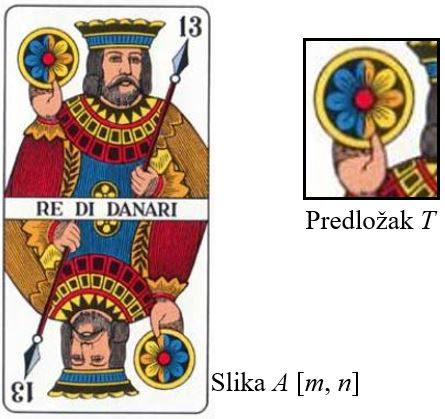
\includegraphics[width=7cm]{./6_PrimjerKrosKorelacije/slika6_1.jpg} 
	\caption{Primjer mogućeg lociranja predloška $T$ na slici $A$}
	\label{sl:6.1}
\end{figure}
\par
Mogući način rješenja problema je da se predložak $T$ "pusti da klizi" po većoj slici $A$, te dalje na svakoj poziciji slike $A$ i predloška $T$ bi se izračunala razlika između predloška i slike (u području preklapanja). Na taj način bi se dobila matrica vrijednosti razlika između predloška i slike, te na mjestu gdje je vrijednost matrice najmanja, najveća je vjerojatnost da je to pozicija predloška. Matematička formulacija opisanog rješenja može biti opisana uz pomoć minimiziranja kvadrata Euklidove duljine (ekvivalentno duljini između dvije točke):
\begin{equation}
	E[i,\, j] = \sum_{m}\sum_{n}\left(A[m,\, n]-T[m-i,\, n-j]\right)^{2}
	\label{eqn:6.1}
\end{equation}
gdje je $A$ slika veličine $[m,\, n]$, a $T$ predložak koji sadrži neku značajku slike $A$ trenutno pozicioniran na lokaciji $i,\, j$. Ako je jednadžba \ref{eqn:6.1} jednaka nuli jasno je kako je pronađena lokacija gdje predložak točno odgovara $i,\, j$ mjestu na slici. Kvadriranjem izraza \ref{eqn:6.1} dobije se:
\begin{equation}
	E[i,\, j] = \sum_{m}\sum_{n}\left(A^{2}[m,\, n]+T^{2}[m-i,\, n-j]-2A[m,\, n]T[m-i,\, n-j]\right)
	\label{eqn:6.2}
\end{equation}
Iz izraza je vidljivo kako je minimiziranje desne strane jednadžbe \ref{eqn:6.1} ekvivalentno maksimiziranju posljednjeg člana iz jednadžbe \ref{eqn:6.2}. Drugim riječima posljednji član (kros-korelacija) jednadžbe \ref{eqn:6.2}  predstavlja mjeru sličnosti između slike $A$ i predloška $T$.
\begin{equation}
	\boxed{R[i,\, j]=\underbrace{\sum_{m}\sum_{n}A[m,\, n]\, T[m-i,\, n-j] = \boldsymbol{T}\otimes \boldsymbol{A}}_{\text{2D kros-korelacija}}}
	\label{eqn:6.3}
\end{equation}
Korištenje izraza \ref{eqn:6.3} kod podudaranja predložaka treba dodatno biti modificirano iz sljedećeg razloga. Za slučaj da "energija" slike $\sum\sum A^{2}(m,\, n)$ varira sa pozicijom, podudaranje koristeći izraz \ref{eqn:6.3} će biti pogrešno. Razlog je u tome što prilikom množenja predloška sa dijelovima slike u kojima predložak ne pripada, može se dogoditi da su vrijednosti slike u tim dijelovima automatski veće nego u dijelu gdje predložak pripada (npr. zbog toga što je u tim dijelovima intenzitet svijetla veći). Tako pomnožene vrijednosti daju u startu veće korelacijske iznose te korištenje kros-korelacije u takvim trenucima nema efekta. Rješenje ovom problemu leži u normalizaciji izraza \ref{eqn:6.3} kojim će se sve automatski velike vrijednosti dovesti na istu razinu u svim područjima slike, tj. energetske razlike unutar slike biti će "ispeglane":
\begin{equation}
	\boxed{N[i,\, j]=\underbrace{\dfrac{\sum_{m}\sum_{n}A[m,\, n]\,T[m-i,\, n-j]}{\sqrt{\sum_{m}\sum_{n}A^{2}[m,\, n]}\sqrt{\sum_{m}\sum_{n}T^{2}[m-i,\, n-j]}}}_{\text{Normalizirana 2D kros-korelacija}}}
	\label{eqn:6.4}
\end{equation}
Lijevi član u nazivniku $\sqrt{\sum_{m}\sum_{n}A^{2}[m,\, n]}$ predstavlja "energiju" slike $A$ u području gdje se slika trenutno preklapa sa predloškom $T$, dok desni član $\sqrt{\sum_{m}\sum_{n}T^{2}[m-i,\, n-j]}$ predstavlja energiju predloška. Na ovaj način kros-korelacija postaje neosjetljiva ne promjene intenziteta slike. \\
U sklopu ovog rada radi lakšeg shvaćanja kros-korelacije u MATLAB-u je odrađen jednostavan primjer pronalaska predloška na slici (primjer sa \textit{Slike \ref{sl:6.1}}) U primjeru je korištena funkcija \textit{normxcorr2} koja prihvaća dva argumenta: prvi argument je predložak, a drugi slika koja će se pretraživati. Oba argumenta moraju biti učitana u obliku slike u sivom tonu. Za slučaj da učitane slike nisu sivom tonu, pozivanjem funkcije \textit{im2gray} slika se prebacuje iz RGB modela boje u sivi ton. Nakon izvršavanja kros-korelacijske funkcije, dobije se korelacijska matrica kojoj je onda potrebno pronaći najveću vrijednost koja u konačnici označava i središte lokacije predloška na slici. MATLAB kod dostupan je u \textit{Prilogu \ref{prilog}1}.
\FloatBarrier
\section{Primjer DPIV kros-korelacije u MATLAB-u}
\label{PIVkod}
U sklopu rada napravljen je i pokazni jednostavni DPIV kros-korelacijski primjer koda (\textit{Prilog \ref{prilog}2}) u svrhu jasnijeg razumijevanja digitalne PIV evaluacije. Za početak učitane su dvije uzastopne PIV snimke, koje su također odmah prebačene u sivi spektar (u ovom primjeru učitane su sintetičke snimke koje su generirane u PIVlab softveru prema postavkama prikazanim na \textit{Slici \ref{sl:6.2}}).
\begin{figure}[h]  
	\centering
	%\usepackage{graphicx}
	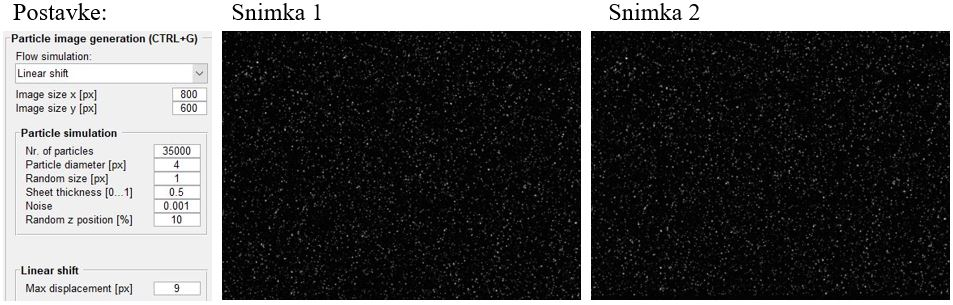
\includegraphics[width=16cm]{./6_PrimjerKrosKorelacije/slika6_2.jpg} 
	\caption{Postavke generiranih snimki u PIVlab-u, kao tip strujanja odabran je linearni pomak prema gore sa maksimalnom vrijednosti pomaka u iznosu od 9 pixela}
	\label{sl:6.2}
\end{figure}
\par
Nakon učitavanja slika u programu je kreirana matrica koja definira prozor ispitivanja, te je odabrana standardna veličina od $64\times 64$ pixela. Naime, kao što je već u ranijim poglavljima objašnjeno, kod PIV kros-korelacije se koristi tzv. strategija podijeli i vladaj (\textit{eng. divide and rule}), prema kojoj se cijela snimka podijeli na mrežu prozora ispitivanja, te se za svaki prozor ispitivanja određuje prosječna brzina svih čestica unutar istoga. Iz toga je jasno kako rezolucija polja brzina ovisi o veličini samog prozora ispitivanja. Da se kreira mreža u programu je još definiran odmak od rubova snimke kojim se osigurava da prozor ispitivanja ne kreće iz ishodišta snimke. Na \textit{Slici \ref{sl:6.3}} grafički su nacrtane dvije uzastopne PIV snimke. Na snimci 1 jasno se vidi odabrani princip generiranja mreže, te treba napomenuti kako mreža u ovom kodu nije centrirana u sredini snimke (pošto nema utjecaja na rješenje), pa razmak između lijeve i desne, odnosno gornje i donje strane nije isti. Čestice na snimci 2 ponovno su pravocrtno pomaknute prema gore.
\begin{figure}[h]  
	\centering
	%\usepackage{graphicx}
	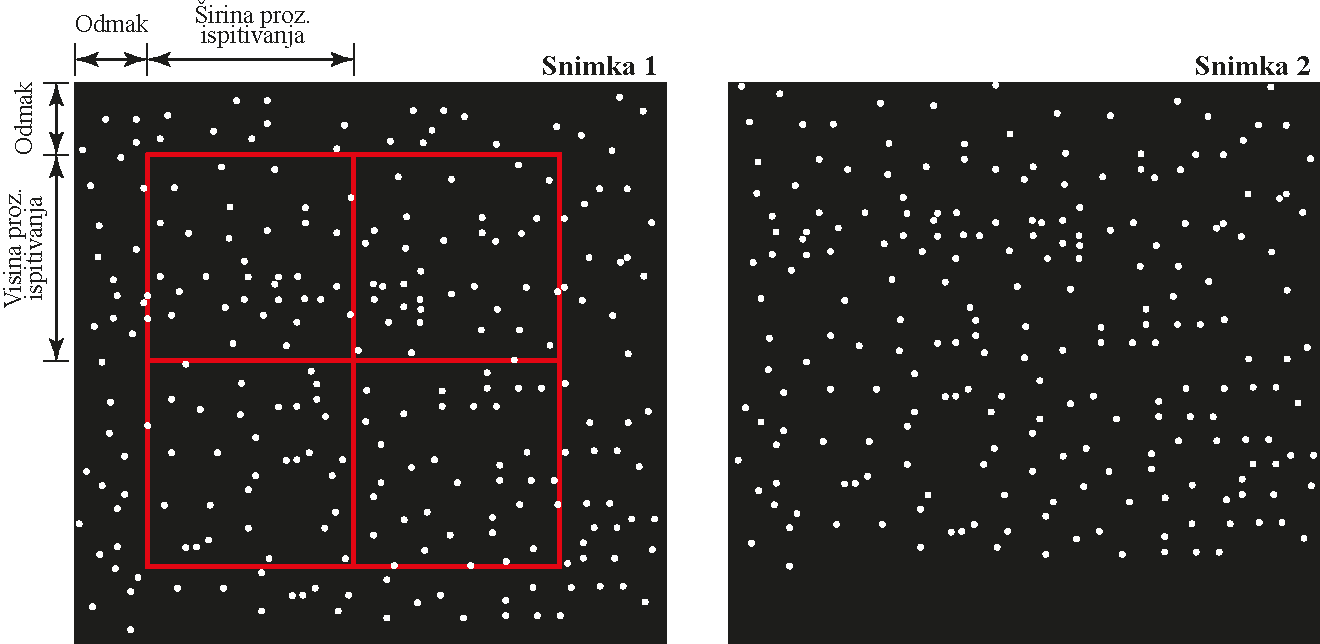
\includegraphics[width=13.5cm]{./6_PrimjerKrosKorelacije/slika6_3.pdf} 
	\caption{Grafički prikaz generiranje mreže koja opisuje prozore ispitivanja, u ovom slučaju postoje 4 prozora}
	\label{sl:6.3}
\end{figure}
\par
Nakon generiranja mreže sljedeći korak je pojedinačna korelacijska analiza svakog prozora ispitivanja posebno. Kros-korelacija se odvija u ugniježđenoj \textit{for} petlji koja se "vrti" ovisno o broju prozora ispitivanja. Laički, sada je cilj pronaći lokaciju manjeg prozora ispitivanja sa snimke 1 na snimci 2, na isti princip kao i u prethodnom poglavlju. U ovom kodu jedina razlika u odnosu na prethodni kod u pretraživanju je ta da se predložak (prozor ispitivanja iz snimke 1) neće pretraživati po cijeloj domeni snimke 2, nego samo u dijelu koji je malo veći od prozora ispitivanja (\textit{Slika \ref{sl:6.4}}). Razlog je u tome što kod PIV mjerenja postoji određena ideja gdje se nalazi predložak na sljedećoj slici, pa bi pretraživanje cijele domene bilo neefikasno. 
\begin{figure}[h]  
	\centering
	%\usepackage{graphicx}
	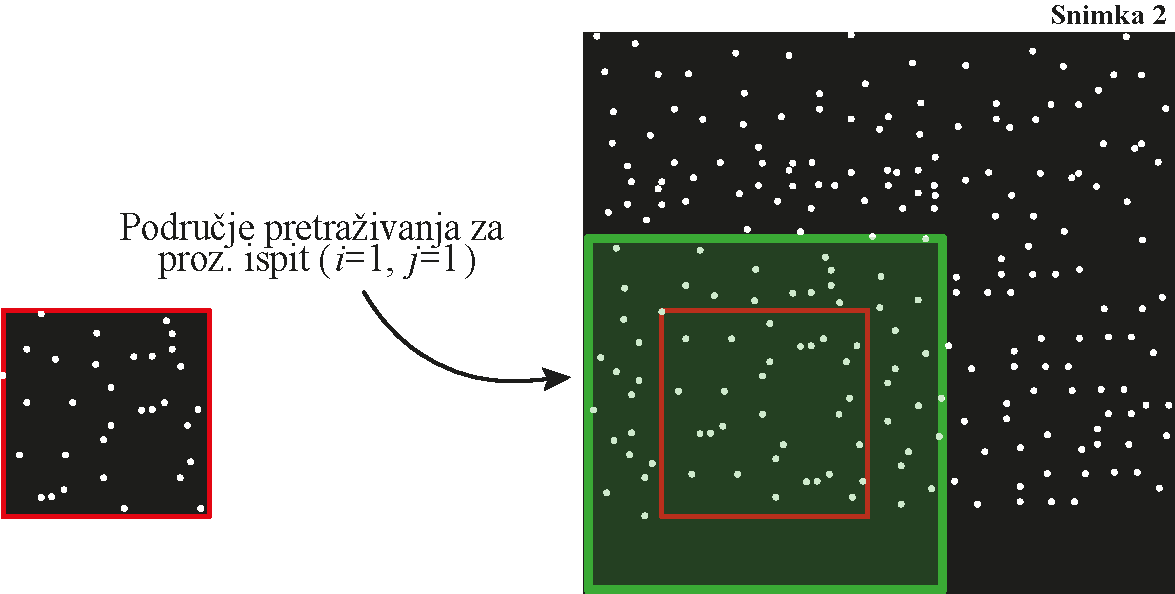
\includegraphics[width=13cm]{./6_PrimjerKrosKorelacije/slika6_4.pdf} 
	\caption{Grafički prikaz područja pretraživanja za prozor ispitivanja $(i=1,\, j=1)$}
	\label{sl:6.4}
\end{figure}
\par
Odabir veličine područja pretraživanja na snimci 2 obično se uzima da bude 2 puta veća od prozora ispitivanja, ali ipak veličina ovisi o parametrima mjerenja, te u skladu s njima mora biti podešena. Za prvu iteraciju \textit{for} petlje područje ispitivanja sa \textit{Slike \ref{sl:6.4}} je ulazni argument u obliku predloška, dok je područje pretraživanja ulazni argument za sliku funkcije \textit{normxcorr2}. Nakon što su slike korelirane, dobije se matrica u kojoj se pronađe najveća vrijednost korelacije, te se koordinate privremeno pohrane da bi se iz njih izračunao pomak koje je jednak razlici koordinata najveće vrijednosti korelacije i koordinatama mjesta prozora ispitivanja. U ovom slučaju postoji samo pomak u y-smjeru (prema gore) kako je prikazano i na \textit{Slici \ref{sl:6.5}}. Sljedeći korak analize je iteracija kroz sve generirane prozore ispitivanja dok se konačno ne dobiju matrice x i y pomaka za sve prozore.
\begin{figure}[h]  
	\centering
	%\usepackage{graphicx}
	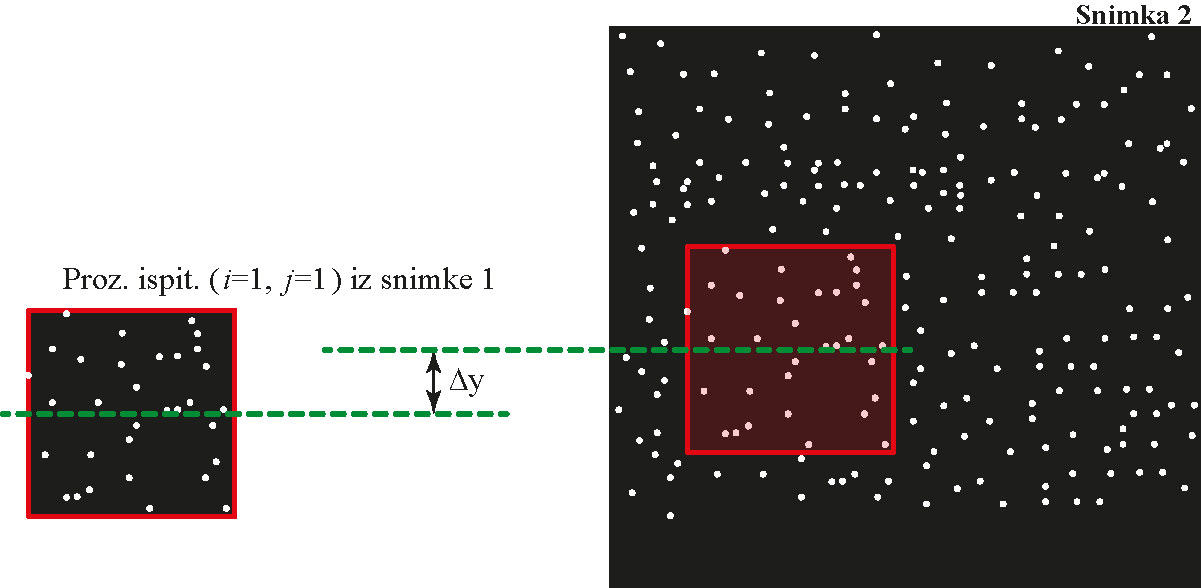
\includegraphics[width=13cm]{./6_PrimjerKrosKorelacije/slika6_5.pdf} 
	\caption{Grafički prikaz dobivenog pomaka}
	\label{sl:6.5}
\end{figure}
\par
Na sljedećim slikama prikazano je nekoliko primjera u kodu izračunanih polja brzina. Na \textit{Slici \ref{sl:6.6}} prikazan je rezultat analize snimki sa \textit{Slike \ref{sl:6.1}}. Na lijevoj slici vidi se primjer analiziran u MATLAB kodu, dok desna slika prikaziva rezultat istih snimki koji je analiziran u PIVlab-u. Kros-korelacija na analiziranoj snimci ispravno je izračunala polje pomaka kod obje analize, te je prosječni iznos svih pomaka 9 pixela, baš kako je i zadano pri generiranju sintetičkih snimki. Iz slika je zanimljivo vidjeti kako PIVlab i na default-nim postavkama pretprocesira analizirane snimke, te pojača kontrast i u suštini pripremi snimke za što kvalitetniju kros-korelacijsku analizu.
\begin{figure}[h]  
	\centering
	%\usepackage{graphicx}
	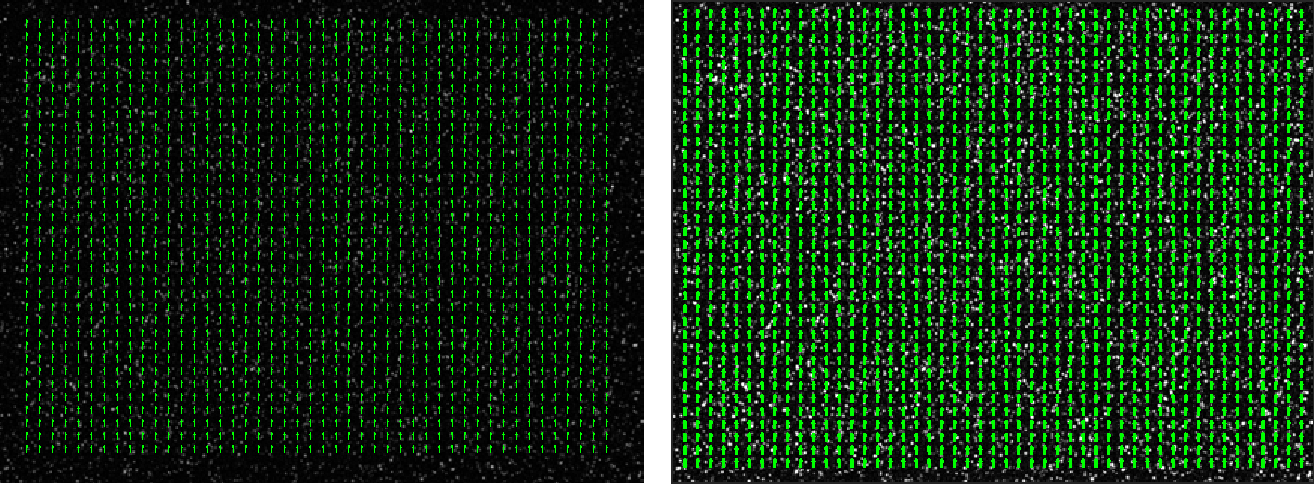
\includegraphics[width=15.5cm]{./6_PrimjerKrosKorelacije/pravocrtnoKodlivoPIVlabdesno.pdf} 
	\caption{Rezultat DPIV kros-korelacije pravocrtnog pomaka čestica u kodu (lijevo) i PIVlab softveru (desno)}
	\label{sl:6.6}
\end{figure}
\par
Na \textit{Slici \ref{sl:6.7}} prikazana je analiza dva Rankine vrtloga \cite{wiki:Rankine} također umjetno generirana u PIVlab softveru. Na slikama je vidljivo kako napisani program već kod malo složenijih strujanja i manje informacijski kvalitetnih snimki daje nepravilne vektore. Dok PIVlab softver uz svoju robusnu pretprocesorsku analizu odlično opisuje polje pomaka dva vrtloga.
\begin{figure}[h]  
	\centering
	%\usepackage{graphicx}
	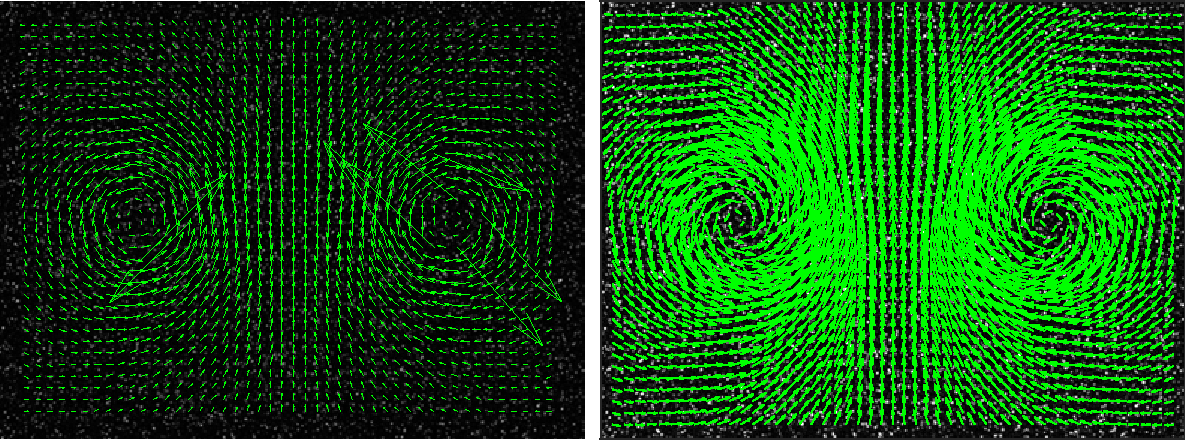
\includegraphics[width=15.5cm]{./6_PrimjerKrosKorelacije/vortexKodlivoPIVlabdesno.pdf} 
	\caption{Rezultat DPIV kros-korelacije dva Rankine vrtloga u kodu (lijevo) i PIVlab softveru (desno)}
	\label{sl:6.7}
\end{figure}
\chapter{DIZAJN I IMPLEMENTACIJA PIV SUSTAVA}
\label{chap:Poglavlje7}
U sklopu rada također je provedena implementacija i jednostavan pokazni primjer mjerenja koristeći PIV sustav. PIV sustav dizajniran je tako da omogući jednostavno korištenje, te minimalan napor za razumijevanje njegovog principa rada, što je i glavni cilj ovog rada u kojem se želi da budući korisnici što lakše poboljšaju znanje iz eksperimentalne i numeričke mehanike fluida. Također, PIV sustav je dizajniran modularno, s ciljem što manjih troškova, sa već dostupnom opremom unutar katedre fakulteta. Tipični komercijalni PIV sustavi danas su izuzetno skupi, sa cijenama od nekoliko desetaka tisuća eura, što dodatno otežava upoznavanje budućih generacija studenata sa PIV mjerenjima. Naravno, pri dizajniranju sustava moraju biti uzete mnoga pojednostavljenja, što limitira korištenje ovog sustava na samo određen broj  tipičnih strujanja (prvenstveno na strujanja u laminarnom području). Tip strujanja fluida ovisi o bezdimenzijskom broju poznatom kao Reynolds-ov broj:
\begin{equation}
	\Reyn = \dfrac{\rho v d}{\mu}
	\label{eqn:7.1}
\end{equation}
gdje $\rho$ označava gustoću fluida, $v$ karakterističnu brzinu strujanja, $d$ karakterističnu duljinu (za strujanje u cijevi, $d$ je promjer cijevi), te $\mu$ dinamičku viskoznost fluida. Pri niskim iznosima Reynolds-ovog broja strujanje teži laminarnom obliku (npr. $\Reyn \leq 2300$ za glatke cijevi), dok pri većim vrijednostima $\Reyn$ broja strujanje prelazi u tranzijentni, odnosno turbulentni oblik. Pri turbulentnom strujanju dolazi do slučajnih fluktuacija koje uzrokuju nepredvidive varijacije, što unosi nesigurnost u mjerenja brzine. Za takva mjerenja potreban je izuzetno robustan i skup, te često posebno dizajniran PIV sustav.\\
Kao što je već objašnjeno, glavne komponente PIV sustava su kamera, laser sa optikom, softver za analizu, te čestice markeri. Sa katedre fakulteta iskorištena je već dostupna brza kamera marke \textit{Chronos 1.4} (\textit{Slika \ref{sl:7.1}}) sa osnovnim karakteristikama rezolucije i fps-a prikazanim u \textit{Tablici \ref{tab:7.1}}. 
\begin{figure}[h]  
	\centering
	%\usepackage{graphicx}
	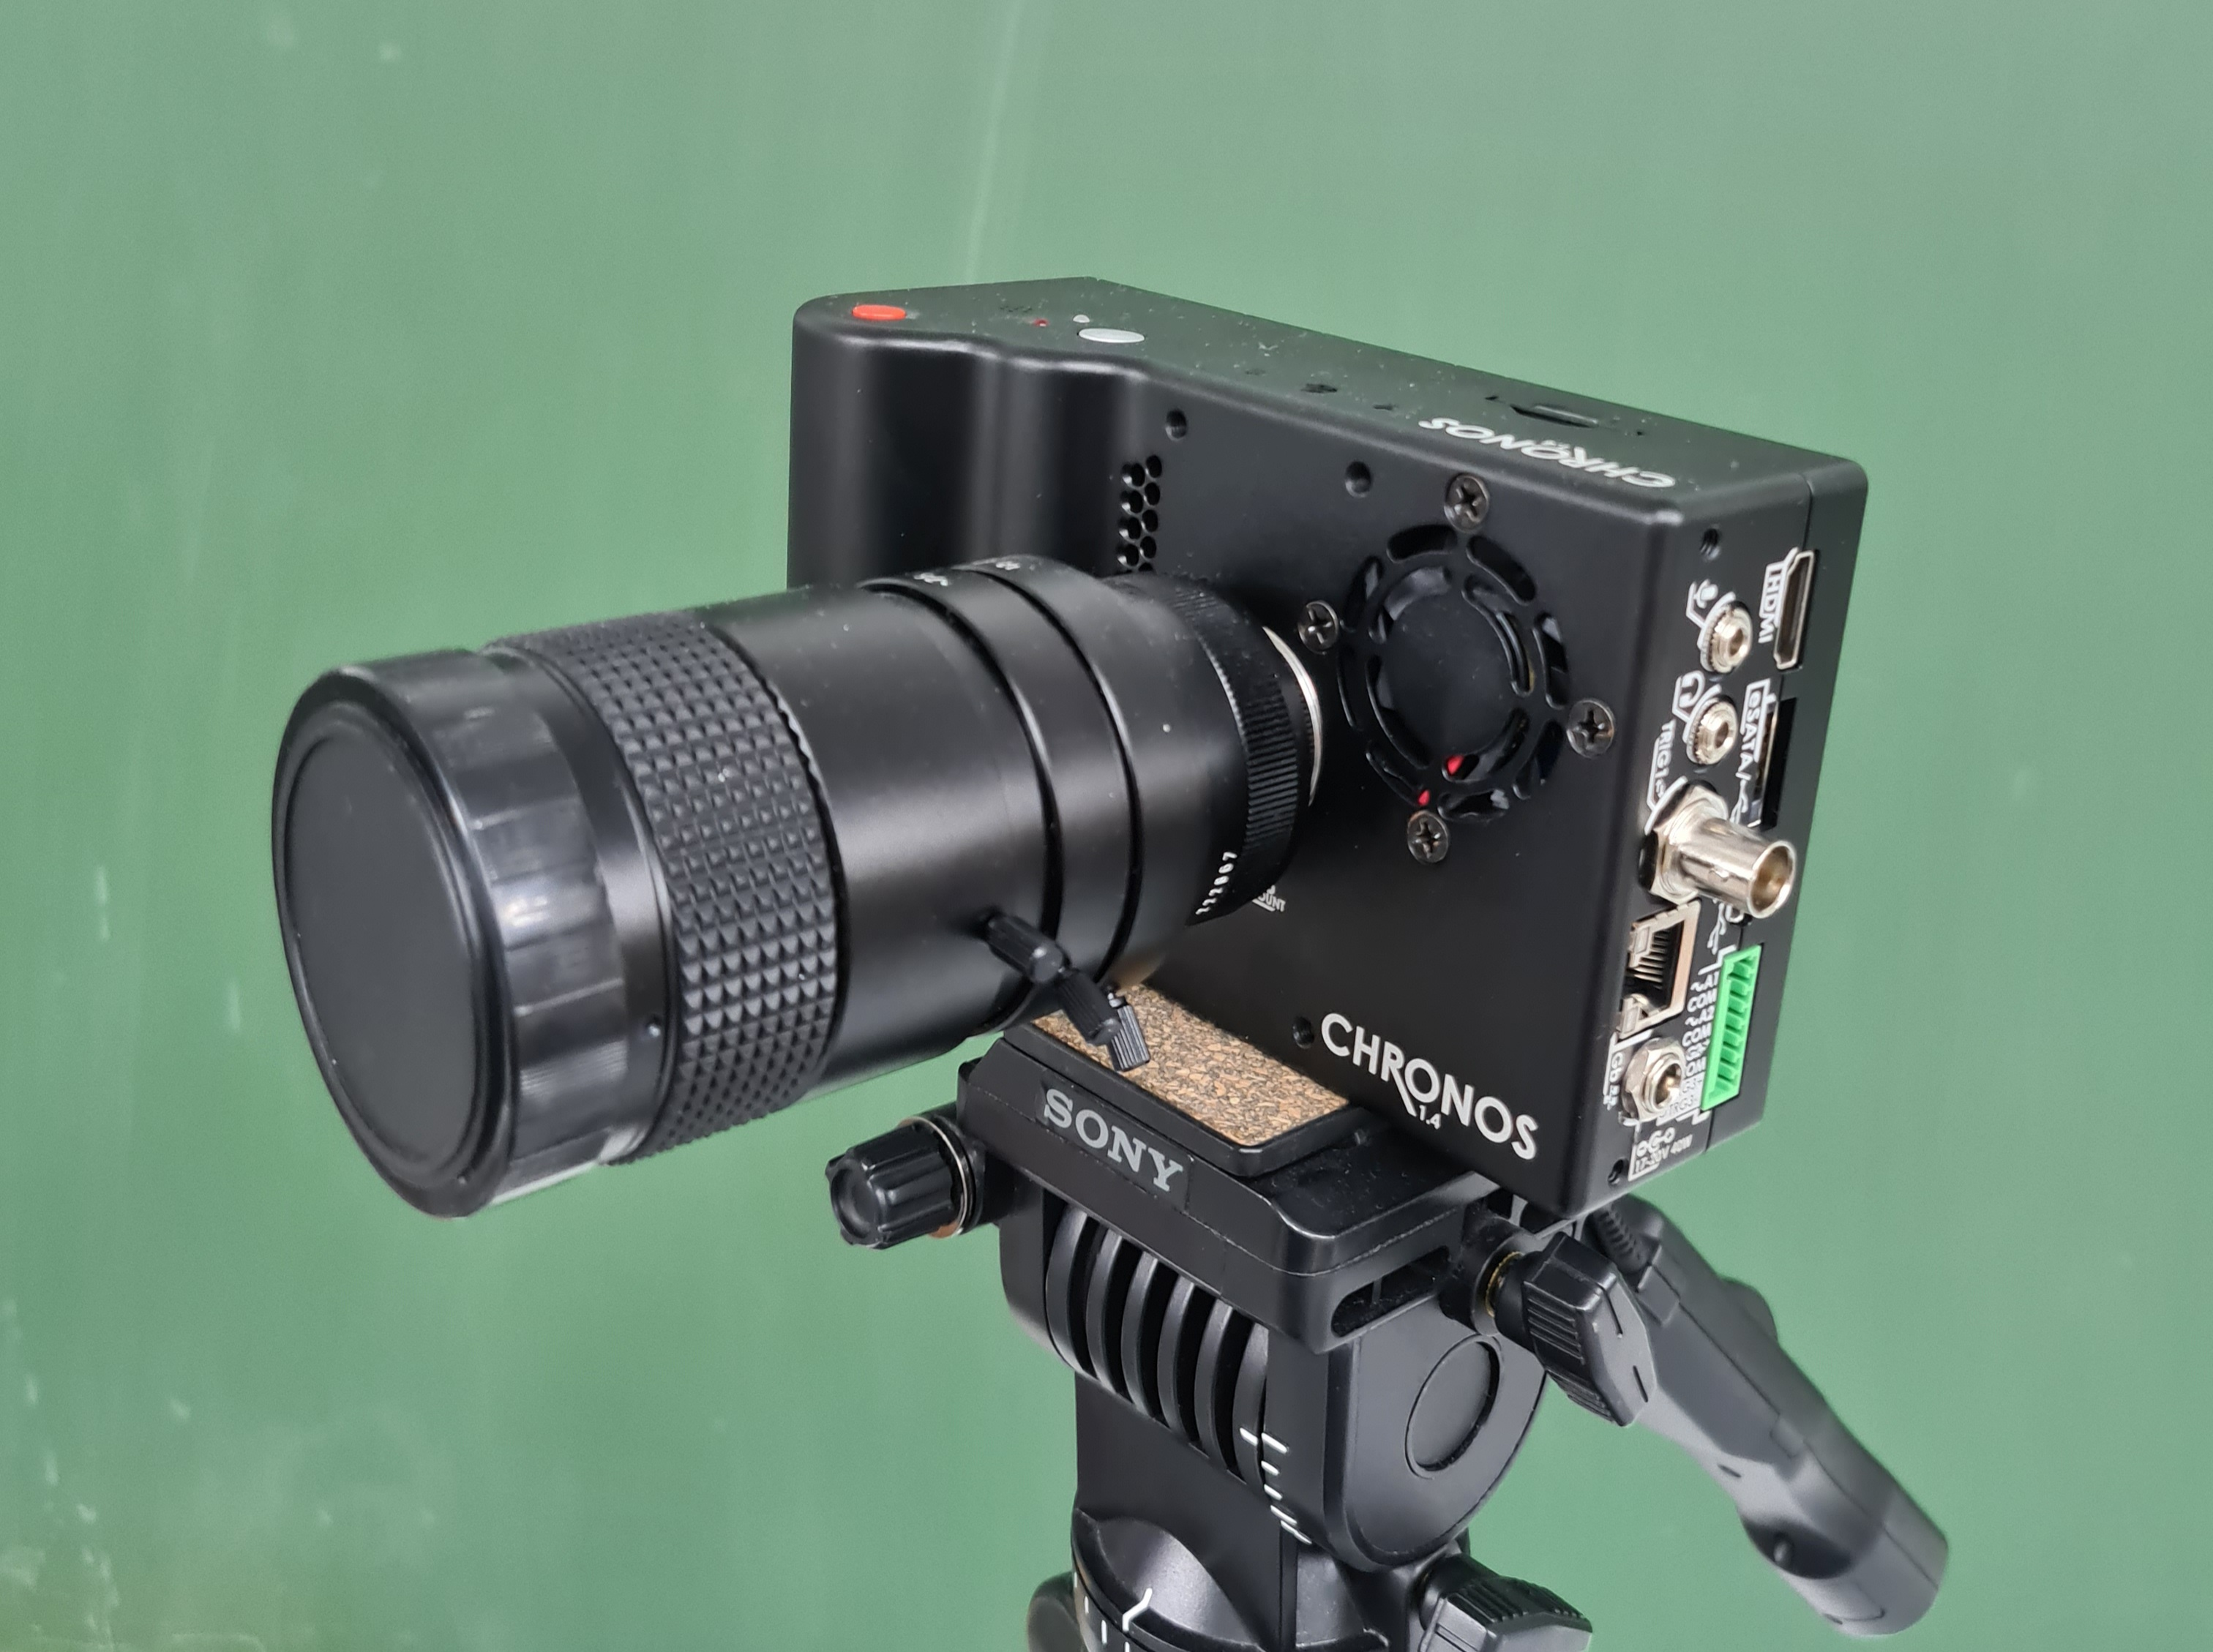
\includegraphics[width=7.4cm]{./7_LowCostPIV/slika7_1.jpg} 
	\caption{Chronos 1.4 brza kamera}
	\label{sl:7.1}
\end{figure}
\par
Kvalitetna kamera u suštini je najbitnija komponenta PIV sustava, te korištena kamera je izuzetno robusna i moguće ju je koristiti kod raznih tipova strujanja uz dodatnu optimizaciju ostalih parametara sustava. Chronos 1.4 je lako prijenosna brza kamera, te ima mogućnost snimanja videozapisa rezolucije $1280\times1024$ pri $1057$ fps-a, a može snimati do $38500$ fps-a pri nižoj razlučivosti. Video se sprema u komprimirani h.264 format ili nekomprimirani RAW format na prijenosni medij (memorijska microSD kartica).
\begin{table}[h]
	\centering
	\caption{Rezolucija i maksimalni broj fps-a za Chronos 1.4 kameru}
	\begin{tabular}{ccc}
		\rowcolor[HTML]{C0C0C0} 
		\textbf{Rezolucija} & \textbf{\begin{tabular}[c]{@{}c@{}}Maks. \\ fps\end{tabular}} & \textbf{\begin{tabular}[c]{@{}c@{}}Vrijeme snimanja \\ (sek.) - 8GB\end{tabular}} \\ \hline
		$1280\times1024$    & 1 057                                                         & 4.13                                                                              \\
		$1280\times720$     & 1 502                                                         & 4.13                                                                              \\
		$1280\times512$     & 2 111                                                         & 4.14                                                                              \\
		$1280\times360$     & 2 999                                                         & 4.14                                                                              \\ \hline
		$1280\times240$     & 4 489                                                         & 4.15                                                                              \\
		$1280\times120$     & 8 923                                                         & 4.17                                                                              \\
		$1280\times96$      & 11 119                                                        & 4.19                                                                              \\
		$1024\times768$     & 1 771                                                         & 4.11                                                                              \\ \hline
		$1024\times576$     & 2 359                                                         & 4.11                                                                              \\
		$800\times600$      & 2 873                                                         & 4.15                                                                              \\
		$800\times480$      & 3 587                                                         & 4.15                                                                              \\
		$640\times480$      & 4 436                                                         & 4.20                                                                              \\ \hline
		$640\times360$      & 5 903                                                         & 4.21                                                                              \\
		$640\times240$      & 8 816                                                         & 4.23                                                                              \\
		$640\times120$      & 17 424                                                        & 4.28                                                                              \\
		$640\times96$       & 21 649                                                        & 4.30                                                                              \\ \hline
		$336\times252$      & 15 200                                                        & 4.43                                                                              \\
		$336\times190$      & 20 020                                                        & 4.47                                                                              \\
		$336\times120$      & 31 192                                                        & 4.53                                                                              \\
		$336\times96$       & 38 565                                                        & 4.60                                                                             
	\end{tabular}
\label{tab:7.1}
\end{table}
\par
Za potrebe laserskog osvjetljenja nabavljen je niskobudžetni laserski modul \textit{CW532-050L} (\textit{Slika \ref{sl:7.2}}). \textit{CW532-050L} je DPSS (diodno upumpavani laser sa čvrstom jezgrom) laserski modul kompaktne veličine koji na sebi ima ugrađenu optiku za generiranje ravnine (linije) pod kutom od 60°. Emitira na valnoj duljini od 532 nm što odgovara zelenoj svjetlosti, te ima optičku izlaznu snagu od 50 mW i automatsku kontrolu snage. Promjer zrake na otvoru (prije linijske optike) iznosi 1.5 mm, te zraka ima divergenciju u iznosu od 1.2 mrad. Optika za generiranje linije je 2'' cilindrična staklena leća. Opisani laser je odabran zbog jednostavnog upravljanja i korištenja koje jedino zahtjeva dodatno napajanje i ponor topline, te je preporučeno korištenje zaštite za vid pri rukovanju sa laserom. Laser također emitira kontinuiranu zraku, pa nije potreban uređaj za sinkronizaciju "puls-eva" lasera i kamere.
\begin{figure}[h]  
	\centering
	%\usepackage{graphicx}
	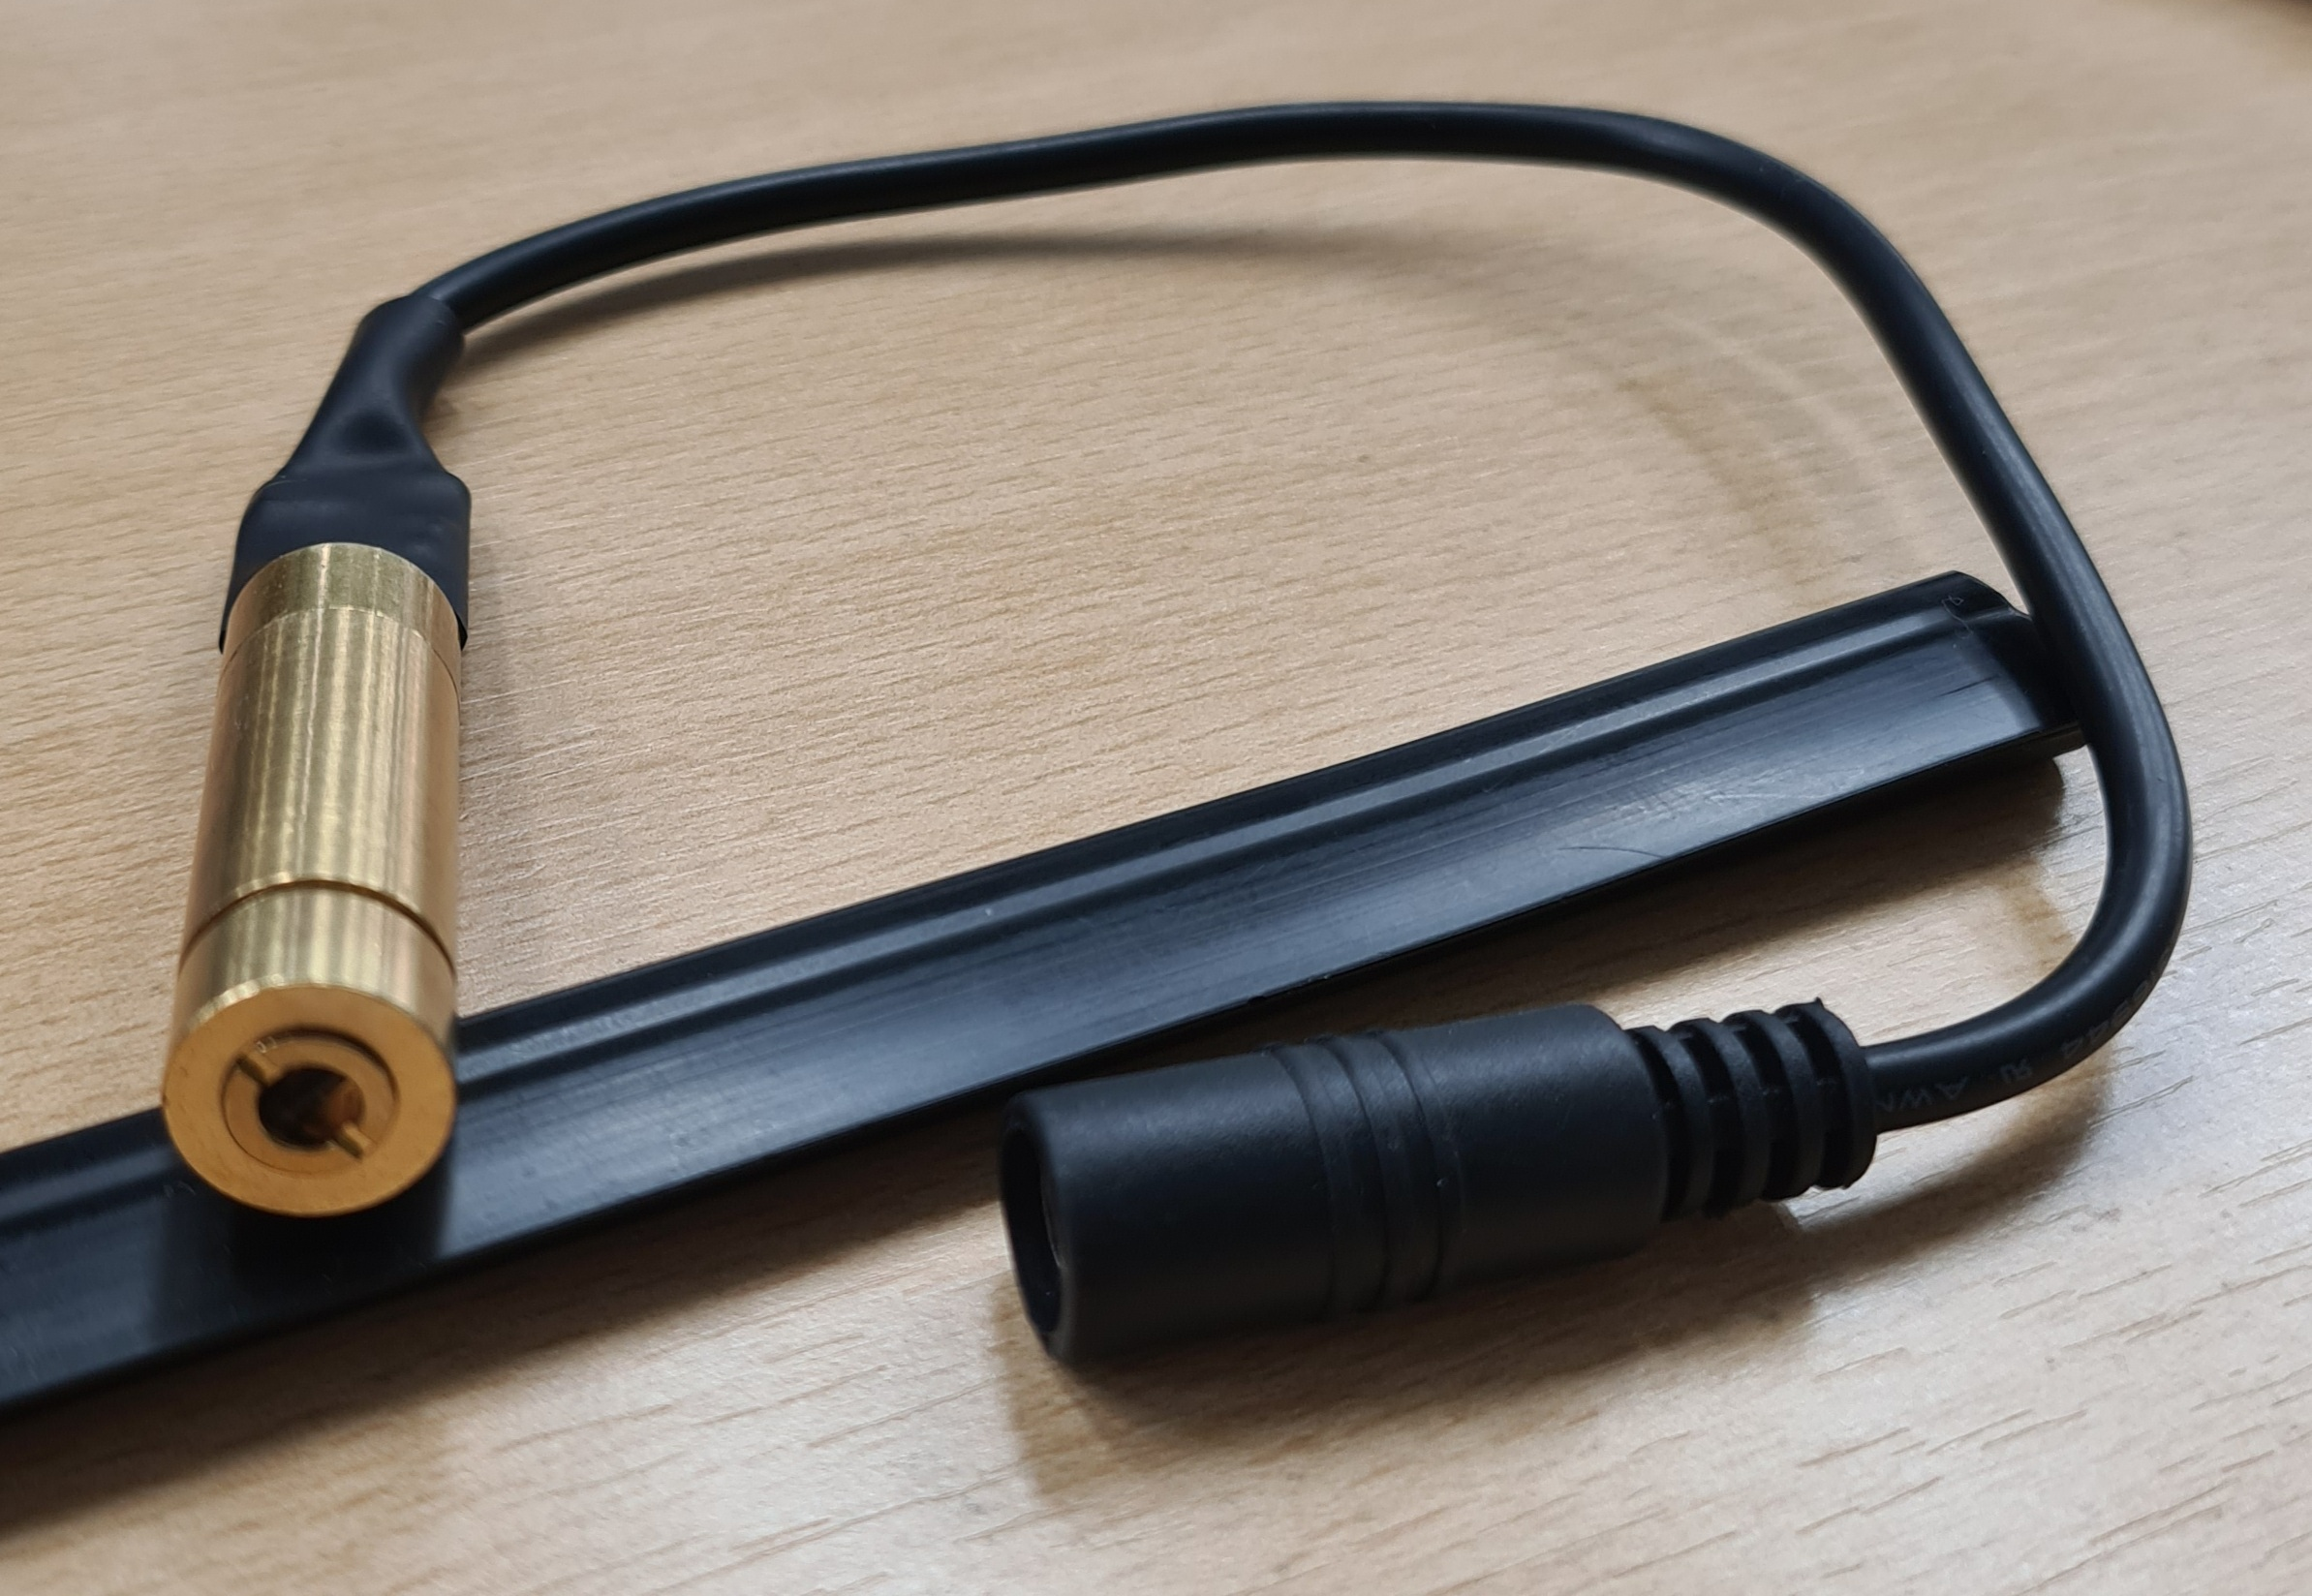
\includegraphics[width=9cm]{./7_LowCostPIV/slika7_2.jpg} 
	\caption{CW532-050L DPSS zeleni laser sa ugrađenom linijskom optikom}
	\label{sl:7.2}
\end{figure}
\par
Kako je dizajniran 2D PIV sustav, kao softver za analizu korišten je PIVlab koji u sebi ima uključene najnovije (\textit{eng. state od the art}) tehnike obrade slike i podataka. Za korištenje PIVlab softvera potrebna je MATLAB licenca koju mnoga sveučilišta obično posjeduju, ali moguće je korištenje i putem studentske licence u vrijednosti cca. 100 \$. Kao što je već ranije opisano PIV mjerenja se obično izvode u vodi ili zraku, pri čemu je u promatrane fluide potrebno dodati čestice markere od kojih će se odbijati laserska svjetlost, te tako označiti strujanje. Pri testnom mjerenju u ovom radu nisu korištene dodatne čestice zbog korištenja vode iz slavine u kojoj već postoje sitne čestice kamenca koje su bile sasvim dovoljne za vizualizaciju strujanja. Naravno, za bilo kakva ozbiljnija mjerenja potrebno je ispravno odabrati čestice markere, te kao preporuku niskobudžetnih čestica moguće je koristiti npr. sitne otpadne čestice pri CNC obradi (za mjerenja u vodi), ili čestice finog škroba (za mjerenja u zraku).
\par
Kao testni pokazni primjer funkcioniranja PIV eksperimenta izabrano je mjerenje brzine istrujavanja iz cijevi promjera 4 mm u spremnik kvadratnog oblika dimenzija $200\times200\times500$ mm (\textit{Slika \ref{sl:7.3}}). U spremnik je dodana voda iz slavine, te je uronjena cijev iz koje istrujava voda, koja se pumpa iz drugog spremnika. Brzina istrujavanja iz cijevi iznosi cca. 3 m/s (nisu uračunati gubici), dok volumni protok pumpe iznosi cca. 2.4 l/min. Kraj cijevi je vertikalno uronjen u vodu, te je laserska ravnina postavljena tako da cijev uzdužno siječe na pola kao što je vidljivo na slici.
\begin{figure}[h]  
	\centering
	%\usepackage{graphicx}
	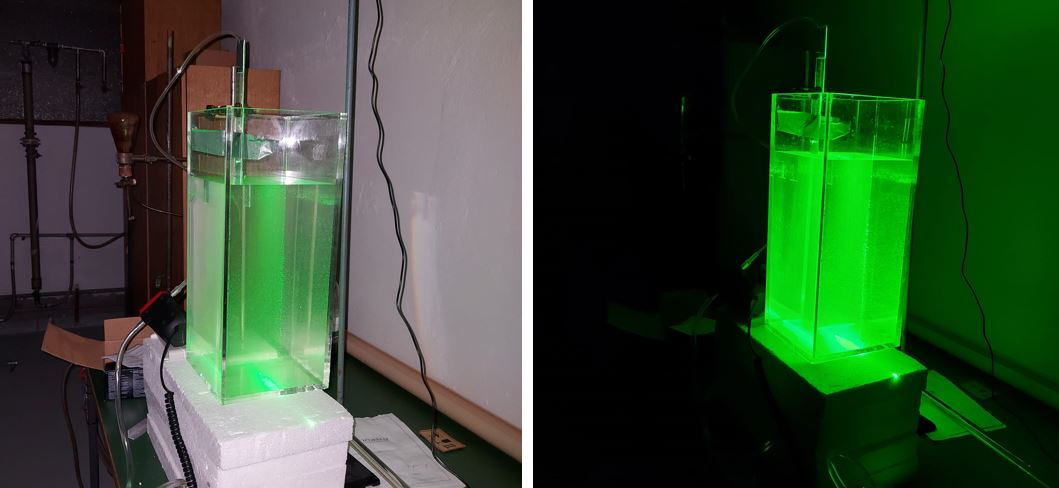
\includegraphics[width=15cm]{./7_LowCostPIV/slika7_3.jpg} 
	\caption{Izgled postavljenog testnog mjerenja}
	\label{sl:7.3}
\end{figure}
\par
Kamera je postavljena normalno na lasersku ravninu, te je namještena najviša moguća rezolucija ($1280\times1024$). Kao brzina stvaranja slike odabrano je 500 fps-a, pokušano je i snimanje sa većim brojem fps-a, ali lasersko osvjetljenje iznad 500 fps-a nije dovoljno snažno da ispravno osvijetli čestice zbog prekratke duljine ekspozicije, te dobivene snimke zbog prevelike količine šuma nisu bile upotrebljive za kros-korelacijsku analizu. Na mjestu gdje laserska ravnina obasjava spremnik postavljena je i mjerna skala koja služi u kasnijoj kalibraciji stvarne duljine domene i duljine domene u ravnini slike (\textit{Slika \ref{sl:7.4}}).
 \begin{figure}[h]  
 	\centering
 	%\usepackage{graphicx}
 	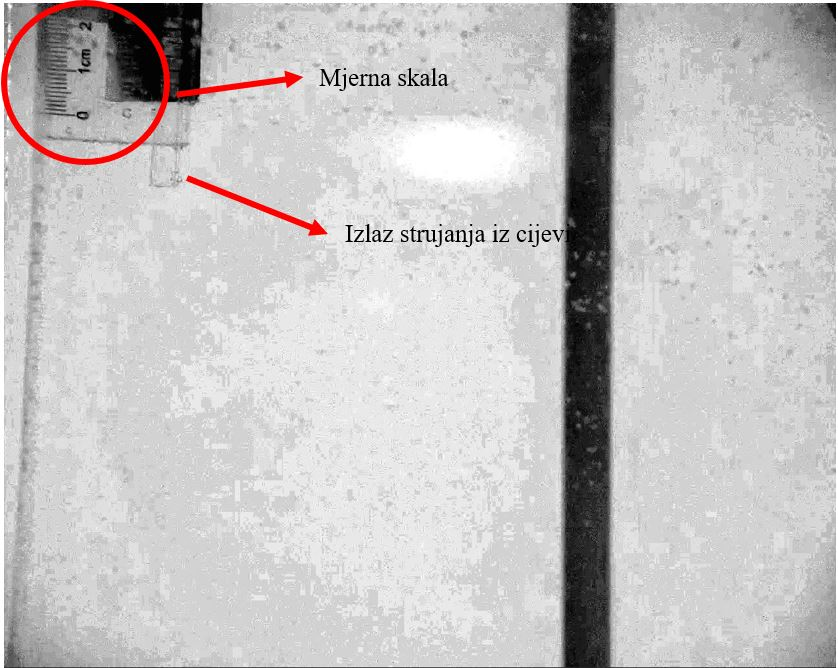
\includegraphics[width=8cm]{./7_LowCostPIV/slika7_4.jpg} 
 	\caption{Kalibracijska snimka kojom se povezuje veličina stvarne domene sa veličinom domene u ravnini slike}
 	\label{sl:7.4}
 \end{figure}
\par
Nakon snimanja akvizicije snimki slijedi prijenos snimki na vanjsku memoriju (microSD) te konačno pohranjivanje na memoriju računala u kojem će se vršiti kros-korelacijska analiza. Prije pokretanja PIVlab programa, uz pomoć open-source VirtualDUB softvera \cite{virtualdub} izvučeno je 50 kadrova (snimke) koje se obliku .mp4 formata u ovom slučaju učitavaju u PIVlab softver.
\begin{description}[style=unboxed,leftmargin=0cm]
	\item[Pretprocesiranje snimki] Kao što je već ranije opisano, PIVlab omogućuje nekoliko tehnika obrade slike kojima se osjetno poboljšati kvaliteta kros-korelacijske analize. Prema zadanim postavkama omogućena je CLAHE tehnika koja lokalno poboljša kontrast u slikama. Također izračunata je prosječna vrijednost pozadine svih 50 kadrova (\textit{Slika \ref{sl:7.6}b}), te je oduzeta od svake snimke posebno što značajno poveća kontrast snimki. Ostale postavljene tehnike prikazane su na \textit{Slici \ref{sl:7.5}}, te je na \textit{Slici \ref{sl:7.6}a} prikazan izgled neobrađene snimke, dok je na \textit{Slici \ref{sl:7.6}c} vidljiv konačan rezultat primjene pretprocesorskih tehnika. Također na \textit{Slici \ref{sl:7.6}c} vidljivo je crveno područje koje je isključeno iz kros-korelacijske analize jer u tom području nema strujanja.
	 \begin{figure}[h]  
		\centering
		%\usepackage{graphicx}
		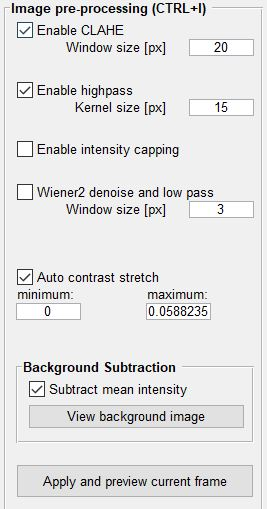
\includegraphics[width=5.5cm]{./7_LowCostPIV/slika7_5.jpg} 
		\caption{Postavljene postavke pretprocesiranja slike u PIVlab softveru}
		\label{sl:7.5}
	\end{figure}
	\begin{figure}[h]  
		\centering
		%\usepackage{graphicx}
		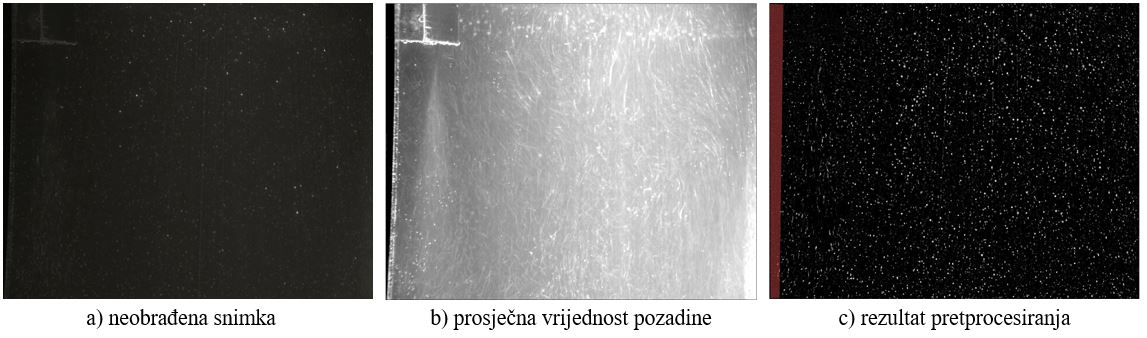
\includegraphics[width=16.5cm]{./7_LowCostPIV/slika7_6.jpg} 
		\caption{Izgled dobivenih snimki: na slici a) prikazana je neobrađena PIV snimka, slika b) prikazuje prosječnu vrijednost pozadine 50 kadrova koji se analiziraju, te se ti kadrovi oduzmu od slike a), dok slika c) prikazuje konačan rezultat obrade snimki}
		\label{sl:7.6}
	\end{figure}
	\item[Opcije PIV analize] PIVlab ima tri različita korelacijska algoritma: DKK (direktnu kros-korelaciju u jednom prolazu), korelaciju skupine snimki (\textit{eng. Ensemble correlation}), te FFT sa tehnikom deformacije prozora. Prema zadanim postavkama omogućen je FFT sa tehnikom deformacije prozora, prvenstveno zbog toga što u većini situacija daje najbolje rezultate. Ovaj algoritam korišten je i u analizi učitanih snimki, te se snimke njime analiziraju u nekoliko prolaza. 
	\begin{figure}[h]  
		\centering
		%\usepackage{graphicx}
		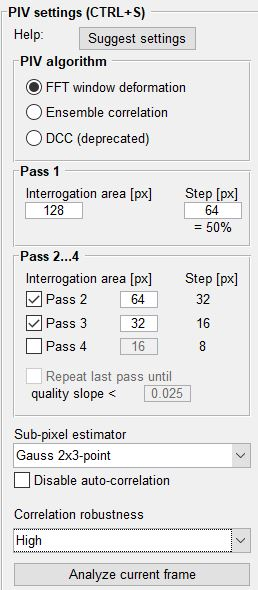
\includegraphics[width=5cm]{./7_LowCostPIV/slika7_7.jpg} 
		\caption{Odabrane postavke za kros-korelacijsku analizu}
		\label{sl:7.7}
	\end{figure}
	\par
	Preporuka je da u prvom prolazu se koristi relativno velik prozor ispitivanja kako bi se pouzdano izračunao pomak podataka sa snimke, jer kao što je već ranije opisano veći prozor ispitivanja daje i veći omjer signala i šuma, te samim time i bolju kros-korelacijsku analizu. Cijena korištenja većih prozora ispitivanja je manja rezolucija vektora brzina, pa je zbog toga korištenje FFT tehnike deformacije prozora mnogo robusnije od ostalih tehnika. Naime u sljedećim prolazima, uzima se manja veličina prozora ispitivanja, te se koriste informacije od prethodnog prolaza kako bi se pomaknulo ispitivanje ("deformiralo" područje ispitivanja) u trenutnom prolazu. Na taj način poveća se vektorska rezolucija (viši DVR), te omjer signala i šuma. Generalna preporuka je korištenje barem 3 prolaza, te nije bitno da oni budu djeljivi sa dva jer MATLAB za korelaciju koristi FFTW koji može "rukovati" sa proizvoljnim veličina prozora ispitivanja. Bitno je samo da se prozori ispitivanja postepeno smanjuju sa brojem prolaza. Također potrebno je napomenuti kako postavljanje iznimno malenog prozora ispitivanja u posljednjem prolazu (npr. $4\times4$ pixela), dovodi do osjetnog smanjenja omjera signal-šum, što dovodi do nesigurnosti u mjerenju, te je zbog toga potrebno oprezno postaviti veličinu posljednjeg prozora ispitivanja. Na \textit{Slici \ref{sl:7.7}} prikazane su korištene postavke pri testnom mjerenju u ovom radu.
	\item[Kalibracija] Nakon analize snimki PIVlab kao jedinicu pomaka koristi "pixel po kadru" (\textit{eng. pixel per frame}), te je potrebna kalibracija kojom se laički softveru kaže koliko se pixela nalazi u jedinici mjere (npr. u metrima), te se zada vremenski korak između kadrova snimki. Na \textit{Slici \ref{sl:7.8}} prikazane su odabrane kalibracijske postavke mjerenja. Odabran je pozitivan smjer x-osi udesno, te pozitivan smjer y-osi prema gore. Na \textit{Slici \ref{sl:7.4}} dodijeljen je razmak od 20 mm pomoću PIVlab grafičkog sučelja i mjerne skale na kalibracijskoj snimci, te je odabran vremenski korak od 2 milisekunde, što odgovara stvaranju snimki pri 500 fps-a. Mjerna skala postavljena je u ravnini laserskog osvjetljenja, te se jednostavno uz pomoć nje povežu stvarne duljina u ravnini lasera i duljina u ravnini slike.
	\begin{figure}[h]  
		\centering
		%\usepackage{graphicx}
		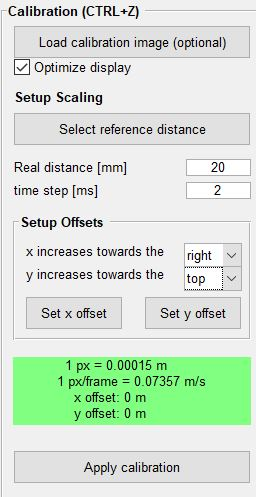
\includegraphics[width=5cm]{./7_LowCostPIV/slika7_8.jpg} 
		\caption{Odabrane postavke za kalibraciju PIV snimki}
		\label{sl:7.8}
	\end{figure}
	\item[Validacija dobivenih podataka] Kako su ovom radu napravljena pokusna testna mjerenja, gdje nisu sasvim dovoljno dobro optimizirani vanjski parametri mjerenja, ovo poglavlje služi kao pokazni primjer pripreme i realizacije PIV eksperimenta. Radi navedenih razloga prilikom kros-korelacijske analize dobiveno je dosta nepravilnih vektora koje je potrebno validirati, te kasnije aproksimirati i zamijeniti što realnim podacima. PIVlab softver ima dvije opcije filtriranja podataka: validacija temeljena na brzini strujanja (\textit{eng. Velocity based validation}), te validaciju temeljenu na podacima sa slike (\textit{eng. Image based validation}). Obično je prilikom provjere dovoljna samo validacija temeljena na brzini gdje se u suštinu odredu gornja i donja granica vrijednosti x i y komponenti brzine. Prilikom odabiranja postavki validacije u ovom radu zadano je samo da lokalne razlike između susjednih vektora brzina budu što manje, tj. zadana je dinamička provjera razlike vektora, tako da je odabrana strogoća filtra brzine iz jednadžbe \ref{eqn:2.10} i \ref{eqn:2.11} u iznosu od 8.
\end{description}
Na sljedećim slikama prikazani su rezultati mjerenja pri 500 fps-a. Na \textit{Slici \ref{sl:7.9}} je vidljivo je dobiveno polje brzina u PIVlab softveru. Kako bi brzina istrujavanja iz cijevi u gornjem lijevom kutu trebala biti cca. 3 m/s jasno je kako korelacijski algoritam nije uspio dobiti dobre brzine. Razlog tome je prvenstveno u previše nasumičnom i turbulentnom 3D istrujavanju iz cijevi. Naime prilikom istrujavanja previše čestica napušta osvijetljenu ravninu te dolazi do prekomjernog izvan-ravninskog gibanja, u kojem se između kadrova gube parovi čestica i korelacijski algoritam ostaje bez uzoraka koje bi trebao povezati. Nadalje kako prilikom mjerenja nisu korištene čestice markeri, nego se na snimkama vide osvijetljene čestice kamenca koje nemaju uniformnu gustoću distribucije, te imaju prevelike razlike u veličini jasno je da dobiveni podaci teško mogu odražavati pravu sliku strujanja, te bilo kakva relevantna mjerenja nisu moguća bez dodavanja čestica markera.
\begin{figure}[h]  
	\centering
	%\usepackage{graphicx}
	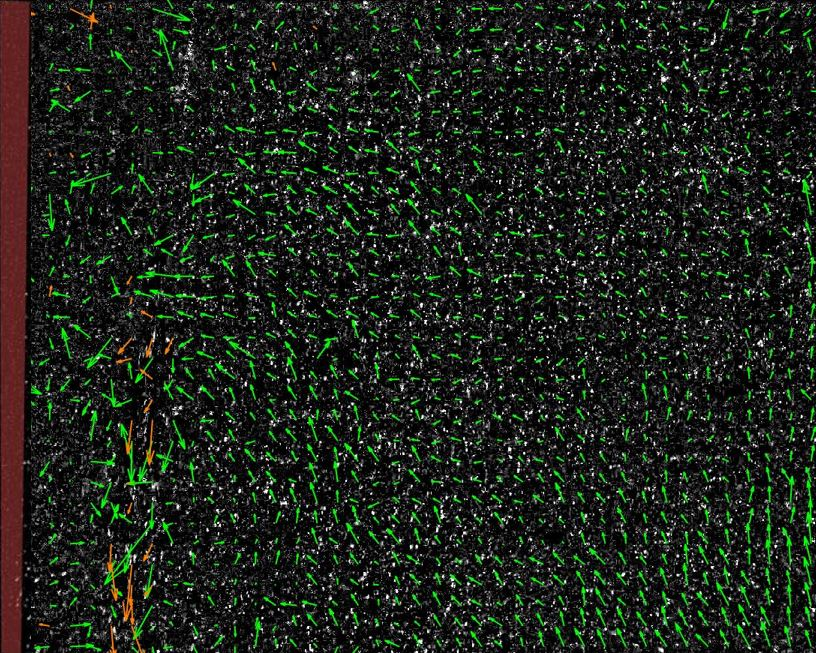
\includegraphics[width=10cm]{./7_LowCostPIV/slika7_9.jpg} 
	\caption{Dobiveno polje brzina u PIVlab softveru (zelenom bojom su označeni izmjereni vektori, a narančastom interpolirani vektori)}
	\label{sl:7.9}
\end{figure}
\par
Dodatni razlog loših rezultata u području istrujavanja je i neujednačena, te jako neuniformna distribucija osvijetljenje u ravninskom smjeru, te u smjeru normalnom na lasersku ravninu. Naime korišteni nisko-budžetni laser nakon samo kratkog rada, osjetno gubi svojstva, te dobivanje što kvalitetnijih mjerenja čini dodatno težim. No ipak rezultati izvan zone istrujavanja čine se dosta boljima i realnijima. Kako je usporenje slojeva vode unutar spremnika dosta intenzivno, dobivene niske brzine u PIV mjerenjima koliko-toliko dosta realnije opisuju polje brzina unutar spremnika. Dobivene komponente brzina u x i y smjeru, moguće je vidjeti na \textit{Slici \ref{sl:7.10}} na $u$-$v$ dijagramu. Iz dijagrama je jasno kako većina $u$ komponenti vektora ima vrijednost između -0.15 m/s i 0.1 m/s, dok $v$ komponenta ide od -0.1 m/s do 0.15 m/s. Dodatni razlog tako niskih brzina je moguća pojava vrtloga na mjestu istrujavanja. Vrtlog se širi u smjeru okomito na snimku te je moguće kako on dodatno prigušuje brzine unutar domene.
\begin{figure}[h]  
	\centering
	%\usepackage{graphicx}
	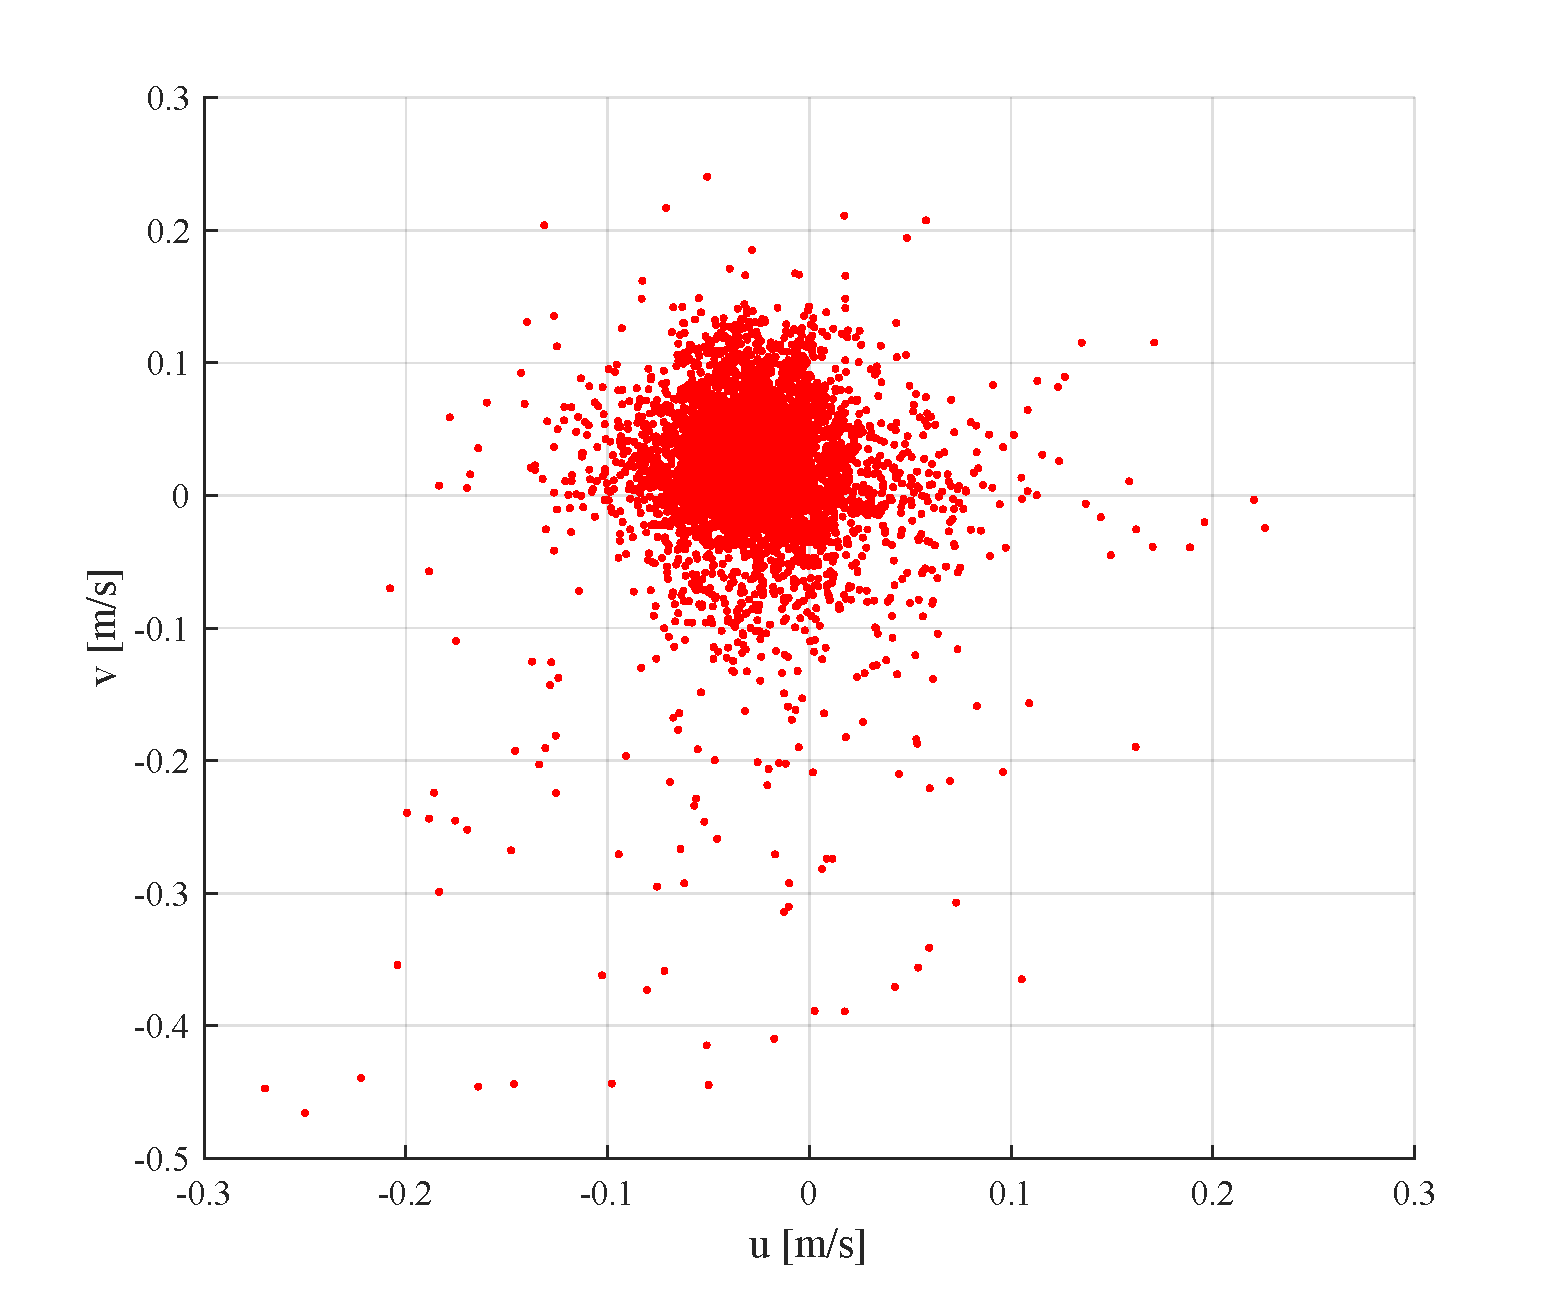
\includegraphics[width=10cm]{./7_LowCostPIV/slika7_10.pdf} 
	\caption{Dobiveni rezultati - $u$-$v$ "scatter" dijagram}
	\label{sl:7.10}
\end{figure}
\par
Na \textit{Slici \ref{sl:7.11}} prikazan je histogram ukupne brzine, te je vidljivo kako najučestaliju frekvenciju pojavljivanja ima brzina malo veća od 0.05 m/s. Ove dobivene podatke jasnije bi trebalo provjeriti sa puno robustnijim PIV sustavom, koji u ovom diplomskom radu nije bilo moguće izvesti, a u suštini to nije bio ni cilj rada. Dodatna provjera rezultata mogla bi  se provesti uz pomoć CFD analize, koja bi uz kvalitetno postavljene parametre simulacije zasigurno mogla omogućiti bolji "osjećaj" za veličine brzina u promatranom strujanju.
\begin{figure}[h]  
	\centering
	%\usepackage{graphicx}
	\includegraphics[width=10cm]{./7_LowCostPIV/slika7_11.pdf} 
	\caption{Dobiveni rezultati - Histogram svih ukupnih brzina strujanja u promatranoj domeni}
	\label{sl:7.11}
\end{figure}

\chapter{ZAKLJUČAK}
\label{chap:Poglavlje8}
Zaključno, u radu je metodologija implementacije PIV tehnologije podijeljena u nekoliko faza. Prikazan je problem evaluacije točnosti DPIV algoritama te su uz pomoć vlastitih umjetnih PIV snimki testirana četiri glavna DPIV algoritma implementirana u PIVlab sustav: DKK, obični DFT te dva DFT algoritma s ugrađenom tehnikom deformacije prozora: multi-linear DFT i multi-spline DFT. Ustanovljeno je kako multi-spline DFT najrobusnije reagira na razne vrste PIV snimki, prvenstveno zbog mogućnosti korelacije u više prolaza te zbog superiornijeg načina interpolacije novih dobivenih prozora ispitivanje (korištenje spline-a). Napisan je jednostavni vlastiti DPIV kros-korelacijski program koji ne sadrži nikakve dodatne tehnike obrade slike te su kvantitativni rezultati korelacijske analize uspoređeni s rezultatima iz PIVlab softvera koji ima mogućnost prethodnog i naknadnog poboljšavanja snimki. U napisanom DPIV kodu koji koristi MATLAB-ovu robusnu korelacijsku funkciju \textit{normxcorr2} i u PIVlab softveru za par analiziranih umjetno generiranih PIV snimki dobiveni su gotovo isti rezultati.
\par
Nadalje, uspješno je dizajniran i implementiran PIV sustav uz pomoć opreme dostupne na katedri fakulteta. Mjereno je istjecanje vode iz cijevi u spremnik pravokutnog oblika dimenzija $200\times200\times500$ mm. Voda je pumpana iz jednog spremnika u drugi, te prosječna brzina istrujavanja iz cijevi iznosi cca. 3 m/s. Napravljene su snimke uz pomoć Chronos 1.4 brze kamere pri 500 fps i rezoluciji snimanja od $1280\times1024$ pixela, korišten je niskobudžetni kontinuirani zeleni laser snage 50 mW koji na sebi ima ugrađenu optiku za generiranje laserske ravnine. U mjerenjima nisu korištene dodatne čestice markeri, nego je korištena voda iz slavine u kojoj je osvjetljeni sitni kamenac služio kao indikator gibanja. Dobivene snimke analizirane su u PIVlab softveru s uključenim opcijama pretprocesiranja snimki, te DFT tehnikom deformacije prozora u 3 prolaza kao DPIV algoritmom. Za veličinu prvog prozora ispitivanja od 128 px, te posljednjeg prozora od 32 pixela dobiveni su najkonkretniji rezultati. DPIV softver nije uspio izmjeriti brzine u zoni istjecanja iz cijevi zbog prevelikog utjecaja (3D) turbulencija. Naime, zbog prebrzog i nasumičnog gibanja na izlazu iz cijevi dolazi do  izvan-ravninskog gibanja čestica, te korelacijski algoritam ne može povezati parove čestica iz dvije uzastopne snimke. Dodatan je problem ne korištenje čestica markera koje bi  povećale korelacijski signal. Također, treba uzeti u obzir nisku kvalitetu korištenog lasera zbog male snage i neujednačenog osvjetljenja. Ipak, uz sve poteškoće prilikom mjerenja, u zoni izvan istjecanja iz cijevi dobiveni su intuitivno realniji rezultati koje i dalje treba uzeti sa dozom opreza. Na kraju je zaključeno kako je moguće korištenje implementirane opreme u daljnjem radu, ali uz uvjet mnogo boljoj optimizaciji parametara snimanja (npr. kontrola snage lasera, korištenje komercijalnih čestica markera, preciznija postavljanje mjerne opreme,...). Jedan od načina provjere dobivenih rezultata bio bi korištenje komercijalne PIV opreme, ili moguća i jednostavnija provjera polja brzina uz pomoć CFD simulacije.

\fancyhead{}
\renewcommand{\headrulewidth}{0pt}
%%%%%%%%%%%%%%%%%%%%%%% LITERATURA / BIBLIOGRAPHY %%%%%%%%%%%%%%%%%%%%%%%%%
%\addcontentsline{toc}{chapter}{Literatura}
\renewcommand{\bibname}{LITERATURA}
\bibliographystyle{unsrturl}
\bibliography{./dipl_literatura}

%%%%%%%%%%%%%%%%%%%%%%% ACRONYMS %%%%%%%%%%%%%%%%%%%%%%%%
\begin{flushleft}

\phantomsection
\addcontentsline{toc}{chapter}{POPIS OZNAKA I KRATICA}
{\Large\bf{POPIS OZNAKA I KRATICA}}
\vskip 10mm
{\large\bf{Oznake}}
\vskip 7mm

\begin{longtable}{rl}
		$"\ast"$ & konvolucijski produkt\\
		$"\otimes"$ & korelacijski produkt\\ 
		$a_{I}$ & područje ispitivanja\\
		$\boldsymbol{a}$ & lokalni vektor ubrzanja\\
		$A$ & površina\\
		$C_{I}$ & prostorna auto-kovarijanca\\
		$C_{II}$ & prostorna kros-kovarijanca\\
		$C_{R}$ & konstantni faktor korelacijske funkcije\\
		$c_{I}$ & prostorni korelacijski koeficijent\\
		$c_{I}$ & prostorni kros-korelacijski koeficijent\\
		$\boldsymbol{D}$ & pomak čestice u vremenu između dva laserska pulsa\\
		$D_{I}$ & područje ispitivanja\\
		$\boldsymbol{d}$ & pomak čestica u ravnini slike\\
		$d_{\textup{č}}$ & promjer čestice\\
		$d_{\tau x},\, d_{\tau y}$ & širina korelacijskih vrhova po x i y smjeru\\
		$E\{ \}$ & očekivana vrijednost\\
		$F_{I}$ & unutar-ravninski gubitak korelacijskih parova\\
		$F_{O}$ & izvan-ravninski gubitak korelacijskih parova\\
		$f(x)$ & funkcija\\
		$I$ & polje vrijednosti intenziteta snimke tijekom prve ekspozicije\\
		$I'$ & polje vrijednosti intenziteta snimke tijekom druge ekspozicije\\
		$I_{0}$ & vrijednost intenziteta svjetlosti odbijene od čestice\\
		$I_{0}(Z)$ & profil vrijednosti intenziteta laserske ravnine po Z-smjeru\\
		$\hat{I},\, \hat{I}'$ & Fourier-ova transformacija $I$ i $I'$\\
		$k_{filter}$ & širina kernel filtra\\
		$M$ & faktor uvećanja\\
		$N$ & ukupan broj\\
		$\Reyn$ & Reynolds-ov bezdimenzijski broj\\
		$R_{C}$ & srednja pozadinska korelacija\\
		$R_{D}$ & vrh pomaka korelacije\\
		$R_{F}$ & član koji opisuje šum zbog slučajne korelacije čestica\\
		$R_{I}$ & prostorna auto-korelacija\\
		$R_{II}$ & prostorna kros-korelacija\\
		$R_{P}$ & samo-korelacija vrha snimke čestice\\
		$R_{\tau}$ & korelacija snimke čestice\\
		$\boldsymbol{s}$ & vektor separacije u korelacijskoj ravnini\\
		$U, \, V, \, Z$ & unutar-ravninske komponente brzine $\boldsymbol{U}$\\
		$\boldsymbol{U}$ & vektor brzine strujanja\\
		$U_{max}$ & maksimalni iznos vektora brzine strujanja u smjeru strujanja\\
		$\boldsymbol{U_{\textup{č}}}$ & brzina čestice\\
		$\boldsymbol{U_{\textup{s}}}$ & zaostajanje brzine\\
		$V_{0}(\boldsymbol{x_{i}})$ & transfer funkcija dana energijom svijetla snimke jedne čestice\\
		$V_{F}$ & volumen fluida u koji su dodane čestice\\
		$W$ & izvan-ravninska komponenta brzine $\boldsymbol{U}$\\
		$W_{0}(X,Y)$ & funkcija przora ispitivanja projektiranog na lasersku ravninu\\
		$X,\, Y,\, Z$ & koordinatni sustav polja strujanja\\
		$x,\, y,\, z$ & koordinatni sustav ravnine snimanja\\
		$\boldsymbol{x}$ & točka u ravnini snimanja, $\boldsymbol{x}=\boldsymbol{x}(x,y)$\\
		$\Delta x_{0},\, \Delta y_{0}$ & dimenzije prozora ispitivanja\\
		$\Delta X_{0},\, \Delta Y_{0}$ & horizontalna i vertikalna dimenzija prozora ispitivanja unutar laserske ravnine \\
		$Z_{0}$ & udaljenost između ravnine objekta i ravnine leće\\
		$z_{0}$ & udaljenost između ravnine snimanja i ravnine leće\\
		$\Delta Z_{0}$ & debljina laserske ravnine\\
\end{longtable}

\vskip 14mm
{\large\bf{Grčke oznake}}
\vskip 7mm

\begin{longtable}{rl}
		$\delta (\boldsymbol{x})$ & Dirac delta funkcija na lokaciji $\boldsymbol{x}$\\
		$\epsilon_{ij}$ & komponente matrice brzine deformacije\\
		$\epsilon_{pristr.}$ & pristrana pogreška\\
		$\epsilon_{slu\text{č}.}$ & slučajna pogreška\\
		$\Gamma$ & cirkulacija\\
		$\Gamma$ & skup\\
		$\mu$ & dinamička viskoznost\\
		$\nu$ & kinematska viskoznost\\
		$\rho$ & gustoća fluida\\
		$\rho_{\textup{č}}$ & gustoća čestice\\
		$\sigma$ & standardna devijacija\\
		$\sigma_{I}$ & prostorna varijanca $I$\\
		$\tau(\boldsymbol{x})$ & PSF funkcija leće za snimanje\\
		$\tau_{\textup{č}}$ & vrijeme odziva čestice\\
		$\omega$ & vektor vrtloženja\\
		$\omega_{x},\, \omega_{y},\, \omega_{z}$ & komponente vektora vrtloženja\\
\end{longtable}

\pagebreak
{\large\bf{Kratice}}
\vskip 7mm

\begin{longtable}{rl}
		1D  &  jedno-dimenzionalni\\
		2D  &  dvo-dimenzionalni\\
		3D  &  tro-dimenzionalni\\
		$\mu$PIV & micro particle image velocimetry\\
		AHE & adaptive histogram equalization\\
		CCD & charge coupled device\\
		CFD & computational fluid dynamics\\
		CLAHE & contrast limited adaptive histogram equalization\\
		CMOS & complementary metal-oxide-semiconductor\\
		DFT & diskretna Fourierova transformacija\\
		DFT multi-lin & diskretna Fourierova transformacija multi linear\\
		DFT multi-sp & diskretna Fourierova transformacija multi spline\\
		DKK & direktna kros-korelacija\\
		DMD & dynamic mode decomposition\\
		DPIV & digital particle image velocimetry\\
		DPSS(L) & diode pumped solid state (laser)\\
		DSR & dynamic spatial range\\
		DVR & dynamic velocity range\\
		eng. & engleski \\
		FFT & fast Fourier transform\\
		fps & frames per second\\
		GPU & graphics processing unit\\
		HPF & high-pass filter\\
		KA & control area - kontrolna površina\\
		LDV & laser Doppler anemometry\\
		LSV & laser speckle velocimetry\\
		Nd:YAG & Neodym-Yttrium-Aluminium-Garnet laser\\
		PCA & principal compoonent analysis\\
		PIV & particle image velocimetry\\
		pixel & picture element\\
		POD & proper orthogonal decomposition\\
		PSF & point spread function\\
		PTV & particle tracking velocimetry\\
		RGB & red green blue\\
\end{longtable}
\end{flushleft}


%%%%%%%%%%%%%%%%%%%%%%%%%%%%%% ABSTRACT %%%%%%%%%%%%%%%%%%%%%%%%%%%%%%%%
\begin{flushleft}
	{\Large\bf{SAŽETAK}}
	\phantomsection
	\addcontentsline{toc}{chapter}{SAŽETAK}
	\vskip 3mm
	{\large\bf{PIV sustav mjerenja brzine strujanja}}	
	\vskip 3mm
\end{flushleft}	
DPIV mjerenje (\textit{eng. digital particle image velocimetry}) nerazarajuća je optička mjerna metoda za dobivanje polja brzina strujanja raznih fluida. Sitne čestice dodaju se uniformno u struju fluida, te služe kao optički markeri preko kojih se može pratiti struja fluida u raznim primjerima. U ovom radu opisuje se 2D DPIV metoda u kojoj se tankom svjetlosnom laserskom ravninom osvjetle čestice koje tako postaju vidljive pri kratkotrajnim ekspozicijama (brze) kamere koja snima određeni broj snimki željene promatrane domene. Analizom dobivenih snimki određuju se pomaci, odnosno brzine strujanja iz kojih se dodatno mogu dobiti ostala fizička svojstva strujanja fluida (tlak, sile na objekte,...).
\par
U uvodu rada prikazana je teoretska pozadina DPIV analize gdje su objašnjena četiri glavna koraka. Prvi korak sastoji se od akvizicije slike gdje su kratko pojašnjena tri glavne potrebne komponente PIV mjerenja: čestice markeri, lasersko osvjetljenje i kamera za snimanje. U drugom koraku objašnjene su najvažnije tehnike pretprocesiranja slike kojima se poboljšava kvaliteta PIV snimki. U trećem, najvažnijem koraku detaljno je pojašnjena evaluacija PIV snimki, te način funkcioniranja kros-korelacijskih algoritama koji se trenutno koriste u najnaprednijim PIV softverima. Kako se čitava PIV analiza temelji na statističkoj kros-korelaciji, u sljedećem poglavlju detaljno je opisana matematička pozadina korelacije jednom ekspozicioniranih snimki. U posljednjem koraku ukratko je opisano postprocesiranje, odnosno validacija dobivenih PIV podataka, te je pojašnjeno dobivanje ostalih fizikalnih svojstava iz polja brzina.
\par
U posljednjem teoretskom, četvrtom poglavlju objašnjena je evaluacija PIV točnosti. Prikazani su najvažniji izvori pogrešaka mjerenja, te parametri koji najviše utječu na kvalitetu korelacijskog signala. Prikazan je način provjere točnosti DPIV algoritama, koji se najčešće vrši generiranjem sintetičkih snimki. Uz pomoć generiranih umjetnih snimki testirani su DPIV algoritmi koji su implementirani u PIVlab softverski paket, te je zaključeno kako u većini slučajeva DFT algoritam s tehnikom deformacije prozora daje najpouzdanije rezultate.
\par
U praktičnom dijelu ukratko je opisana arhitektura i način rada PIVlab softvera. U MATLAB-u napisan je jednostavni DPIV kros-korelacijski kod, te je uz pomoć njega objašnjen način funkcioniranja kros-korelacije. U programu je testirano par umjetnih snimaka, a rezultati mjerenja uspoređeni su s rezultatima iz PIVlab softvera koji je uz uključene pretprocesorske tehnike dao slične rezultate kao vlastiti program. Na kraju rada dizajniran je i implementiran vlastiti PIV sustav uz pomoć opreme dostupne na katedri fakulteta. Demonstriran je proces PIV mjerenja, te je ostvareno pokazno testno mjerenje u kojem se promatra istrujavanje vode iz cijevi. Dobiveni su polu-realni rezultati koji se trebaju uzeti s oprezom zbog mnogih pojednostavljenja i pretpostavki prilikom dizajniranja sustava. Za sam kraj ističe se preporuka nabavke kvalitetnije opreme, te što bolje optimizacije parametara mjerenja prilikom dizajniranja sustava.
\vskip 3mm
\begin{flushleft}	
{
	\normalsize{\bf{Ključne riječi:\\}}
	\textnormal{PIV, DPIV, kros-korelacija, PIVlab, digitalna obrada slike, prepoznavanje uzorka}
}	
\end{flushleft}


%%%%%%%%%%%%%%%%%%%%%%%%%%%%%% ABSTRACT %%%%%%%%%%%%%%%%%%%%%%%%%%%%%%%%
\begin{flushleft}
	{\Large\bf{SUMMARY}}
	\phantomsection
	\addcontentsline{toc}{chapter}{SUMMARY}
	\vskip 3mm
	{\large\bf{Particle image velocimetry (PIV) flow measurement system}}	
	\vskip 3mm
\end{flushleft}	
Digital Particle Image velocimetry (DPIV) is non-intrusive optical measurement method in which main goal is to obtain vector velocity field in fluid flow. Small particles are introduced uniformly into fluid flows and serve as optical markers through which flow can be monitored in various examples. This thesis describes a 2D PIV technique in which a thin laser light plane is illuminated rendering the particles, which become visible in short-time exposures of a (fast) camera, which captures a certain number of images of the desired observed domain. By analyzing the obtained images, it is possible to determine flow velocities from which various other physical properties can be additionally obtained
\par
In the introduction to the thesis, the theoretical background of the DPIV analysis is presented, where four main steps of PIV measurments are explained. The first step consists of image acquisition in which three main components of PIV are briefly presented: tracer particles, laser illumination and camera setup. The second step explains the most important image processing techniques that improve the quality of PIV images. In the most important, third step, the evaluation of PIV images is explained in detail, as well as the working principle of cross-correlation alghoritams used by "state-of-the-art" PIV softwares. As the entire PIV analysis is based on statistical cross-correlation, the following chapter in detail describes mathematical background of the correlation of single-exposed images. In the last step, the post-processing, validation of the obtained PIV data is briefly presented, and the principle of obtaining other physical properties from the velocity field is described.
\par
In the last theoretical, fourth chapter, the evaluation of PIV accuracy is explained. The most important sources of measurement errors are presented, as well as the parameters that mostly influence the quality of the correlation signal. The method for evaluating the accuracy of DPIV algorithms, which is most often done by generating synthetic images, is presented. With the help of generated synthetic particle images, DPIV algorithms which are implemented in the PIVlab software were tested, giving the conclusion that for the most cases "window deformation DFT" gives the most reliable results.
\par
The practical part briefly describes the architecture and principle of operation of PIVlab software. A simple DPIV cross-correlation code was written in MATLAB, and it was used to explain how cross-correlation works. A couple of synthetic particle images were tested in the program, and the measurement results were compared with the results from the PIVlab software, which, with the included preprocessor techniques, gave similar results as written program. At the end of the paper, an low-cost PIV system was designed and implemented with the equipment available at the faculty department. The PIV measurement process was demonstrated, and test measurement was performed in which the flow of water from the pipe is observed. Quasi-realistic results have been obtained that need to be taken with caution, due to many simplifications and assumptions when designing the system. At the end, it is concluded that for more serious measurments, better equipment is needed which also needs to be accompanied with the best possible optimization of measurement parameters.

\vskip 3mm
\begin{flushleft}	
	{\setstretch{1.1}
		\normalsize{\bf{Keywords:\\}}
		\textnormal{PIV, DPIV, cross-correlation, PIVlab, digital image processing, pattern recognition}
	}	
\end{flushleft}


%%%%%%%%%%%%%%%%%%%%%%%%% PRILOG / APPENDIX %%%%%%%%%%%%%%%%%%%%%%%%%%%
\phantomsection
\addcontentsline{toc}{chapter}{PRILOG}
\chapter*{PRILOG}
\fontsize{12pt}{1.5pt}\selectfont

\large\bfseries
\begin{enumerate}[style=unboxed,leftmargin=0cm]
\item[1.] MATLAB kod - podudaranje predloška sa slikom (\textit{Pogl. \ref{podudaranjePredlSlika}})
\label{prilog}
%\fontsize{12pt}{1.5pt}
%\noindent\rule{16cm}{0.2pt}
\lstset{language=Matlab,%
	basicstyle=\footnotesize\color{red},
	%basicstyle=\color{red},
	breaklines=true,%
	morekeywords={matlab2tikz},
	keywordstyle=\color{blue},
	morekeywords=[2]{1}, keywordstyle=[2]{\color{black}},
	identifierstyle=\color{black},
	stringstyle=\color{mylilas},
	commentstyle=\color{mygreen},
	showstringspaces=false,%without this there will be a symbol in the places where there is a space
	numbers=left,%
	numberstyle={\tiny \color{black}},% size of the numbers
	numbersep=9pt, % this defines how far the numbers are from the text
	emph=[1]{for,end,break},emphstyle=[1]\color{red}, %some words to emphasise
	emph=[2]{word1,word2}, emphstyle=[2]{style},    
}

%\subsection*{MatLab kod za izracun trokutastog KE}
\lstinputlisting{./MATLAB_kod/DIPkomande.m}
%\noindent\rule{16cm}{0.2pt}
\vskip 0.42cm
%\newpage 
\item[2.] MATLAB kod - DPIV kros-korelacija (\textit{Pogl. \ref{PIVkod}})
\lstinputlisting{./MATLAB_kod/mojaPIVanaliza.m}

\end{enumerate}


\end{document}